\documentclass{article}
\usepackage[utf8]{inputenc}
\usepackage[english]{babel}
\usepackage{algorithm}
\usepackage{algpseudocode}
\usepackage[letterpaper, left=0.8in, right=0.8in, bottom=1in, top=0.75in]{geometry}
\usepackage{parskip}
\usepackage[citestyle=authoryear]{biblatex}
\usepackage{csquotes}
\addbibresource{footer/ref.bib}
\usepackage{amsmath}
\usepackage{amssymb}
\usepackage{appendix}
\usepackage{hyperref}
\usepackage{cleveref}
\usepackage{lmodern}
\usepackage[T1]{fontenc}
\usepackage{textcomp}
\usepackage{stmaryrd}
\usepackage{xparse}
\usepackage{tabularx}
\usepackage{graphicx}
\usepackage{float}
\usepackage{array}
\usepackage{siunitx}
\usepackage[acronym, toc, section,numberedsection=autolabel]{glossaries}


\makeatletter
\algrenewcommand\ALG@beginalgorithmic{\footnotesize}
\makeatother
\algrenewcommand\algorithmicrequire{\textbf{Input:}}
\algrenewcommand\algorithmicensure{\textbf{Output:}}

\setlength{\parskip}{1em}
\renewcommand{\baselinestretch}{1.2}
\newcommand{\textbox}[1]{\fbox{\parbox{\dimexpr\linewidth-2\fboxsep-2\fboxrule\itshape}{#1}}}
\setlength{\fboxsep}{1em}

\newtheorem{theorem}{Theorem}[section]
\newtheorem{corollary}{Corollary}[theorem]
\newtheorem{lemma}[theorem]{Lemma}

\newcolumntype{C}{>{\centering\arraybackslash}X}
\newcolumntype{L}{>{\raggedleft\arraybackslash}X}
\newcolumntype{R}{>{\raggedright\arraybackslash}X}

\makeglossaries

%TC:ignore
%TC:ignore
\newglossaryentry{tree}{
    name={Tree (graph theory)}, 
    text={tree}, 
    description={A graph with a tree structure is defined as a connected graph where any two vertices are connected by exactly one path}
}

\newglossaryentry{approx_algs}{
    name={Approximation Algorithms},
    text={approximation},
    description={algorithms that produces a solution with a provable guarantee to be within a certain distance to the optimal solution. The guarantee is expressed as a multiplicative factor, for example a $n$-approximation algorithm will always return a solution equal to or less than $n$ times the cost of the optimal solution. Another common notation used is a $\mathcal{O}(1)$-approximation, which does not define a specific approximation factor but states that the approximation factor does not grow with the size of the input}
}

\newglossaryentry{randomised_algs}{
    name={Randomised Algorithms},
    text={randomised},
    description={a type of algorithm which relies on randomness to make decisions; typically the aim is to use randomness to reduce the the time complexity of the algorithm}
}

\newglossaryentry{genetic_algs}{
    name={Genetic Algorithms},
    text={genetic},
    description={a metaheuristic inspired by natural selection, it maintains a population which is used to create offspring for each generation}
}

\newglossaryentry{heuristic}{
    name={Heuristic},
    text={heuristic},
    plural={heuristics},
    description={a "rule of thumb" strategy for solving a problem which aims to lead to a good solution. The strategy is problem dependent}
}

\newglossaryentry{metaheuristic}{
    name={Metaheuristic},
    text={metaheuristic},
    plural={metaheuristics},
    description={a higher level strategy for solving a problem which is independent of the problem it is trying to solve, which serves as a framework for designing heuristics}
}

\newglossaryentry{local_search}{
    name={Local Search},
    text={local search},
    description={a metaheuristic where we are given a candidate solution, and our search space are neighbours of the candidate solution; the objective of the search is to find a neighbour solution better solution than the current solution}
}

\newglossaryentry{pseudo_approximation}{
    name={Pseudo Approximation Algorithm},
    text={pseudo approximation},
    description={an approximation algorithm which may break a constraint in order to achieve its specified approximation factor}
}

%TC:endignore
%TC:ignore

\newacronym{pbs}{PBS}{Population Based Search}
\newacronym{vns}{VNS}{Variable Neighbourhood Search}
\newacronym{grasp}{GRASP}{Greedy Adaptive Randomised Search Procedure}
\newacronym{grasp_ps}{GRASP-PS}{Greedy Adaptive Randomised Search Procedure (Plateau Surfer)}
\newacronym{ml}{ML}{Machine Learning}
\newacronym{ipco}{IPCO}{Integer Programming and Combinatorial Optimization}
\newacronym{lp}{LP}{Linear Program}
\newacronym{ui}{UI}{User Interface}
\newacronym{ga}{GA}{Genetic Algorithm}
\newacronym{ma}{MA}{Memetic Algorithm}
\newacronym{js}{JS}{JavaScript}
\newacronym{xpm}{xPM}{Exact Perfect Matching}
\newacronym{html}{HTML}{Hyper Text Markup Language}
\newacronym{d3}{D3}{Data Driven Document}
\newacronym{ux}{UX}{User Experience}
\newacronym{uuid}{UUID}{Universally Unique Identifier}

%TC:endignore
%TC:endignore

\begin{document}
%TC:ignore
\begin{titlepage}
    \setlength\headheight{90pt}
    \begin{center}
        \begin{figure}[h!]
            \centering
            
\includegraphics[width=0.25\textwidth]{images/uob.png}
        \end{figure}
        
        \vspace{0.25cm}
            {\scshape\LARGE University of Birmingham \par}
            \vspace{0.25cm}
            {\scshape\Large Final year project\par}
        \vspace{0.5cm}
        
        \centering
        \Large{\textbf{On the $k$-center and Colourful $k$-center}}
        
        \vspace{1cm}
        \Large{\textit{Timothy Cheung}}
        
        \normalsize{School of Computer Science}
        
        \vspace{1cm}
        Supervised by\par
        Dr. Rajesh Chitnis \\
        School of Computer Science\par
        \vspace{1.5cm}
        
        \large{May 2021}
    \end{center}
\end{titlepage}
\newpage
\newpage
\begin{abstract}
The k-center problem is a classical \gls{combinatorial_optimisation} problem with applications in machine learning and real world applications such as warehouse location. The $k$-center problem aims to allocate at most $k$ facilities to n clients such that the distance the furthest client has to travel to their nearest center is minimised. In recent years, there has been a increase interest in fairness constraints on classical theoretical problems. This led to the introduction of the colourful $k$-center problem. Given a data set with a split demographic, the colourful $k$-center adds constraints where a minimum number of individuals from each demographic must receive service from the set of centers. We are interested in fairness constraints because the classical algorithms may have inbuilt biases which lead them to exclude service from certain groups.

This paper aims evaluate the performance of approximation algorithms and metaheuristic approaches on the $k$-center and colourful $k$-center problems. To date, the colourful $k$-center has only been studied from a theoretical viewpoint, therefore we contribute two new data sets for the colourful $k$-center problem to study it from an empirical viewpoint. The first is GOWALLA (a 3D data set based on real world data) and the second is SYNTHETIC (a 2D artificial data set with known optimal solutions). Finally, we present a \gls{memetic_algs} algorithm, a \gls{genetic_algs} algorithm which utilises a local search, which solves the colourful $k$-center problem. We observed that our algorithm produces solutions with an average of 48.6\% lower cost than existing algorithms.

Furthermore, we develop a web tool for algorithm visualisation. It aims to educate the user about $k$-center problems, visualise solutions and provides a step by step high level overview of how the algorithms work.
\end{abstract}
\newpage

\newpage
\tableofcontents
\newpage
%TC:endignore
\section{Introduction}
In the recent years the term Big Data has become more relevant, it is defined as data which is too large to process using traditional methods. Even in 2008, Google processed over 20 petabytes of data per day (\cite{dean_mapreduce_2008}). There is a strong motivation for improving the techniques used in handling Big Data, since it has real world applications in fields such as medicine, transportation and city planning (\cite{al_nuaimi_applications_2015,obermeyer_predicting_2016}). 

Machine learning is often applied to analyse and organise these large sets of data. In the realm of machine learning, the two overarching paradigms for processing data are supervised and unsupervised learning. Supervised learning involves data sets which are labelled with the ground truth, whereas unsupervised learning does not require labelled data. Classification is a supervised learning method where given a set of categories, we make use of the labelled data set with the goal of creating a function which predicts the category of an unseen example. Conversely, clustering attempts to group together similar data points. 

There are several approaches to clustering, including centroid, density and connectivity based models. In centroid based models, the data points are partitioned based on specific points designated as centers; each data point is assigned to a center to minimise some dissimilarity metric. Some common centroid based clustering methods are $k$-means, $k$-median, and $k$-center. These clustering problems NP-hard, which means given that $P\neq NP$, there does not exist an algorithm which runs in polynomial time which also produces an optimal solution. As generating clusters poses considerable complexity and computational cost, there is interest in the development of new methods for traditional clustering problems (\cite{zhao_parallel_1970}). 

In this paper we explore centroid based clustering, specifically the $k$-center and its variations. The $k$-center problem is a classical \gls{combinatorial_optimisation} problem first proposed by \textcite{hakimi_optimum_1964}. Its goal is to cluster points together such that the distance between the point farthest from its nearest center is minimised. In the literature for solving the k-center problem there are broadly three types of algorithms: \gls{exact_algs} (which give an optimal solution), \gls{approx_algs} (which give a guarantee of solution cost) and \glspl{metaheuristic} (which provide no such guarantee).

The $k$-center problem has been traditionally studied with the requirement that all points must be part of a cluster, however \textcite{charikar_algorithms_2001} identified that a small amount of outliers can cause a large increase in the optimal cost. This resulted in them introducing the robust $k$-center problem which considers the scenario where a minimum number of points must be clustered (rather than all of them). Consequently, further generalisations of the Robust $k$-center problem have been formulated, the colorful $k$-center problem divides the points in colour groups and the minimum number of points from each colour group which must be part of a cluster is specified (\cite{bandyapadhyay_constant_2019}). This work is part of a larger trend of investigating bias and fairness in traditional machine learning approaches (\cite{mehrabi_survey_2019, anegg_technique_2020}).

The $k$-center problem has been typically applied to facility location problems, where we are given a set of clients and we have to allocate them to $k$ facilities to minimise the distance of the farthest candidate to its nearest facility. However, it has also seen relevance in more a novel applications, such as rendering images with natural lighting (\cite{agarwal_structured_2003}) and summarising a collection of images subject to fairness constraints (\cite{kleindessner_fair_2019}).

This project will explore the various approaches to solving the $k$-center and colourful $k$-center problems.

%The remainder of the paper is structured as follows. The next section is a review of the literature on the $k$-center problem and its variants and descriptions the algorithms at a high level. \Cref{section:background} is a detailed description of the algorithms which we have implemented. In \cref{section:design} we describe the design of our tool to to visualise these algorithms. \Cref{section:results} evaluates the performance of the algorithm using empirical methods; in particular, we investigate the running time and analyse the distance between the solution cost to the optimal cost. Finally in \cref{section:evaluation}, we provide evaluation of our algorithm and tool, then discuss potential extensions in \cref{section:discussion}.

\section{Literature Review}\label{section:lit_review}

    \subsection{Overview}
    In this literature review we will cover the history of the $k$-center problem, first introduced by \textcite{hakimi_optimum_1964} and the subsequent variants introduced by \textcite{charikar_algorithms_2001} and \textcite{bandyapadhyay_constant_2019}. We give formal definitions for the $k$-center, Robust $k$-center and Colourful $k$-center problems provide real world analogies to contextualise them. Following this, we show some novel applications of the $k$-center problem and then describe traditional and modern approaches to solving the $k$-center and Colourful $k$-center problems.
    
    \subsection{The \texorpdfstring{$k$}{k}-center problem}\label{section:k_center}
    The problem setting for the $k$-center problem  is an undirected weighted graph $G=(V,E)$ on $n$ vertices. The weight of an edge between two vertices $v_1, v_2$ is given by a function $dist(v_1,v_2)\rightarrow\mathbb{R}_{\ge 0}$. The distance function must satisfy triangular inequality; the sum of any two sides of a triangle is less than or equal to the length of the remaing side. In the context of graphs, given any three vertices the following holds for any pair of vertices: \(dist(a,b) \leq dist(a, c) + dist(b, c) \).

\textcite{hakimi_optimum_1964} first introduced two problems: the absolute center and the vertex center of a weighted undirected graph. The absolute center considers any point $x$ on an edge and therefore defines a more general distance metric between two points along any two edges; this metric is given by a function $pdist(x_1,x_2)\rightarrow\mathbb{R}_{\ge 0}$ which is the sum of the path between the two points (since a point can lie inbetween an edge, the path can contain a partial edge). The goal is to find a point $c$ which minimises the maximum $pdist(c,x_i)$ for all points along the edges. In contrast the vertex center restricts the center candidates to vertices in $G$. Therefore the goal is to find a vertex $c$ which minimises the maximum $dist(c, v_i)$ for all vertices $v_i\in V$. It should be noted that in the remainder of this paper, when we refer to center type problems, we are referring to the vertex center rather than the absolute center. 

\textcite{hakimi_optimum_1965} published further work one year later which generalised the absolute and vertex center problems, by considering the allocation of $k$ centers rather than a single center; the original problem definition can be thought of as the 1-center problem. The $k$-center problem can be thought of as a facility location problem, where we want to locate $k$ facilities in order to best service the $n$ clients. The clients $N$ and potential location for facilities $M$ are subsets of the vertices, such that $N\subseteq V$ and $M\subseteq V$. We consider the scenario where every vertex can either be a client or a facility, where $M=N=V$. The $k$-center problem can therefore be defined more formally as follows:

\textbox{Given a graph $G=(V, E)$ on a set of $n$ vertices $V = \{v_1,..., v_n\}$ and a parameter $k$ specifying the maximum number of centers (where $1\leq k\leq n$): 

\vspace{0.2cm}We want to find a subset of centers $C\subseteq V$ such that $|C|\leq k$ which minimises the objective function: $max_{v\in V}min_{c\in C}dist(v, c)$}

An alternative way to describe this problem would be to imagine a city where we would like to build warehouses for a parcel delivery service. Given a destination for a parcel, the parcel will depart from the warehouse nearest to the destination. The city would like to build these warehouses in the optimal locations such that the largest distance a delivery driver will have to travel is minimised. Now consider that the city has a limited budget and they can only build \(k\) warehouses. In this scenario, we want to allocate $k$ warehouses to minimise the distance between the house that is furthest away from its nearest warehouse.

Later work showed that while solving the vertex 1-center problem is a trivial process, solving the $k$-center problem for graphs of arbitrary structure is NP-hard (\cite{kariv_algorithmic_1979}). Their worked focused on a simplified version of the $k$-center problem, where the graph has a tree structure. A graph with a tree structure is defined as a connected graph where any two vertices are connected by exactly one path. \textcite{kariv_algorithmic_1979} reported a $\mathcal{O}(n^2\cdot log(n))$ algorithm which solves the $k$-center problem on trees.

Given the NP-hardness of the $k$-center problem, there exists no algorithm with gives an optimal solution which also runs in polynomial time. Therefore when designing algorithms for NP-hard problems, we either aim to give an optimal solution in exponential time or a non-optimal solutions in polynomial time. Throughout this paper, when we refer to a solution for the $k$-center problem (and its variants) we are referring to a valid solution which may or may not have the optimal cost. In the literature for the $k$-center problem, the latter forms the majority of the studies. The primary algorithm paradigms applied to the $k$-center problem include approximation algorithms, randomized algorithms, metaheuristics and local search techniques. We define these paradigms below:
\begin{itemize}
    \item \textbf{Approximation algorithms}: a type of algorithm that returns a solution with a provable guarantee to be within a certain distance to the optimal solution. The guarantee is expressed as a multiplicative factor, for example a $n$-approximation algorithm will always return a solution equal to or less than $n$ times the cost of the optimal solution. Another common notation used is a $\mathcal{O}(1)$-approximation, which does not define a specific approximation factor but states that the approximation factor does not grow with the size of the input. 
    \item \textbf{Heuristic}: a "rule of thumb" strategy for solving a problem which aims to lead to a good solution. The strategy is problem dependent.
    \item \textbf{Metaheuristics}: a higher level strategy for solving a problem which is independent of the problem it is trying to solve, which serves as a framework for designing heuristics.
    \item \textbf{Local search}: a metaheuristic where we are given a candidate solution, and our search space are neighbours of the candidate solution; the objective of the search is to find a neighbour solution better solution than the original candidate.
    \item \textbf{Randomized algorithms}: a type of algorithm which relies on randomness to make decisions; typically the aim is to use randomness to reduce the the time complexity of the algorithm.
    \item \textbf{Genetic algorithms}: a type of algorithm inspired by natural selection, it maintains a population which is used to create offspring for the next generation.
\end{itemize}

Several approximation algorithms have been proposed to solve the $k$-center problem, the most widely cited are is the \emph{Gon} algorithm (\cite{gonzalez_clustering_1985}) and the \emph{HS} algorithm (\cite{hochbaum_best_1985}) which both produce 2-approximations; they are described in detail in \cref{section:greedy}. The \emph{Gon} algorithm is based on a greedy heuristic and the \emph{HS} is based on a binary search. Furthermore, \textcite{hochbaum_best_1985} proved that the $k$-center problem is not only NP-hard to solve optimally, but it is also NP-hard to approximate to for any approximation factor less than 2.

One of the more influential metaheuristics for combinatorial optimisation is VNS (Variable Neighbourhood Search), first introduced by \textcite{mladenovic_variable_1997}. The basic concept of VNS is to use local search to explore the current neighbourhood of solutions, and to switch neighbourhood if better solutions than the incumbent is found. The VNS metaheuristic was later applied to the $k$-center problem by \textcite{mladenovic_solving_2003}. Given an incumbent solution $C$, the neighbourhood structure is defined as solution $C$ with each facility replaced by every other potential facility making the cardinality of $N(C)$ equal $k\times (n-k)$. To efficiently implement this, data structures were designed to store, for each client, the closest and second closest facility to it. Their application of the VNS metaheuristic resulted in a $\mathcal{O}(i\cdot n^{2})$, where $i$ is the number of VNS iterations. \textcite{mladenovic_solving_2003} evaluated their algorithm on the OR-LIB problem instances, a standard data set originally used for $k$-median problems (\cite{beasley_note_1985}) later adapted for the $k$-center. Their empirical results showed that the VNS algorithm significantly outperformed the \emph{Gon} and \emph{HS} approximation algorithms.

Later publications built upon the VNS algorithm, the neighbourhood structures created by \textcite{mladenovic_solving_2003} were used in the PBS (Population Based Search) algorithm (\cite{pullan_memetic_2008}). PBS is a metaheuristic which aims to generate starting points to run local search on. To do this it uses a memetic algorithm, an extension of a genetic algorithm which conducts a local search on the individuals of the population. Their work showed the ability to converge to the optimal cost in the OR-LIB data set where VNS could not.

To the best of our knowledge, the most recent literature using search based techniques proposed for solving the standard $k$-center problem is the Plateau Surfer algorithm (\cite{battiti_new_2017}). Their work builds upon the observations by \textcite{mladenovic_solving_2003} of $k$-center solutions which have equal cost but different vertices forming the furthest vertex from its nearest center. They observed that these solutions of equal cost could trap the search in a local minima, and proposed algorithms to escape these minima. They reported that their algorithm produced near optimal solutions faster than state of the art local search techniques for the $k$-center.

While both the PBS (\cite{pullan_memetic_2008}) and Plateau Surfer algorithm (\cite{battiti_new_2017}) were reported to have better performance than VNS (\cite{mladenovic_solving_2003}), \textcite{battiti_new_2017} did not compare the PBS algorithm to their Plateau surfer algorithm; in our study we will implement both and compare their performance. The PBS and the Plateau Surfer algorithms are discussed in further detail in \cref{section:pbs} and \cref{section:plateau_surfer} respectively.
    
    \subsection{The robust \texorpdfstring{$k$}{k}-center problem}\label{section:robust_k_center}
    The robust $k$-center problem (also known as the $k$-center problem with outliers) extends $k$-center problem by introducing a constraint \(p\) (\(1 \leq p \leq n \)) which specifies the minimum number of clients that must be serviced the centers (\cite{charikar_algorithms_2001}). This problem is more applicable to real scenarios, for example in our parcel delivery service analogy (\cref{section:k_center}), there may be houses on the outskirts of the city which are not profitable to deliver to (since the clients are less concentrated in that area); we may want to exclude them when building the warehouses. Therefore the city can change their requirements and ask to build $k$ warehouses such that 80\% of the city's population lives in a reasonable distance away from their nearest warehouse. Note that when \(p=n\), we have the $k$-center problem.

Formally, this problem can be stated as follows:

\textbox{Given a graph $G=(V, E)$ on a set of $n$ vertices $V = \{v_1,..., v_n\}$, a maximum number of centers $k$ and a minimum coverage constraint $p$ (where $1\leq k\leq n$ and $1\leq p\leq n$):

\vspace{0.2cm}We want to find a subset of centers $C\subseteq V$ which covers a subset of vertices $Z\subseteq V$ such that $|C|\leq k$ and $|Z|\geq p$ which minimises the objective function: $max_{v\in Z}min_{c\in C}dist(v, c)$}

\citeauthor{charikar_algorithms_2001} proposed a 3-approximation algorithm in $\mathcal{O}(n^{3})$ time. They note that the cost of the solution must be one of the $n^{2}$ interpoint distances in $\{d(i,j)\mid i\in V, j\in V\}$. Their method is to perform a binary search on the interpoint distances, then at each iteration evaluate a cost $r$; given a radius $r$ to check, greedily choose a center that cover the most points the most uncovered points within the distance $r$ and expand this to $3r$, marked these points as covered and repeat until $k$ centers are chosen. The search looks for the smallest radius $r$ which covers more than $p$ points. For a more detailed description of this algorithm we refer the reader the original paper by \textcite{charikar_algorithms_2001} and a later paper which discussed implementation optimisations by \textcite{schwartz_efficient_2010}.
    
    \subsection{The colourful \texorpdfstring{$k$}{k}-center problem}\label{section:colourful_k_center}
    The colourful $k$-center problem (\cite{bandyapadhyay_constant_2019}) is a generalisation of the Robust $k$-center problem. It introduces $\emph{c}$ new parameters which represent the demographic that each client belongs to. The set of clients V is partitioned into $\emph{c}$ classes, $V=\{V_1,... V_{\emph{c}}\}$, and for each class $\emph{i}$ at least $1\leq t_i \leq |V_i|$ clients must be covered. Note when $\emph{c}=1$, we have the robust $k$-center problem.

In the parcel delivery service analogy, excluding clients is not detrimental. However, imagine performing facility location for an essential service such as hospital location for ambulances. If we have some prior knowledge of the clients, for example suppose people aged over 60 tend to be more medically vulnerable and live on the outskirts of the city. Solving the robust $k$-center for this scenario will neglect people aged over 60, since the robust $k$-center biased towards denser clusters. Therefore the hospitals will be located further away from a group that is more likely to require the ambulance service. Instead if we apply the colourful $k$-center problem and partition the clients into $\emph{c}=2$ groups (aged over and under 60), we can specify that we would like to cover 100\% of clients aged over 60 and 80\% of clients under 60. Solving the colourful $k$-center problem under these constraints will produce an allocation of hospitals which corrects for the bias.

This can be formally stated in the following:

\textbox{Given a graph $G=(V, E)$ on a set of $n$ vertices $V = \{v_1,..., v_n\}$, colour classes $1,...,c$, where the vertices are partitioned into the colour classes $V_1, ...,V_c$, a maximum number of centers $k$ and we are given a minimum coverage constraint corresponding to each colour class $t_1,...,t_c$ (where $1\leq k\leq n$ and $\forall _{i\in\llbracket 1\mathrel{{.}\,{.}}\nobreak c\rrbracket}$ $1\leq t_i\leq n$): 

\vspace{0.2cm}We want to find a subset of centers $C\subseteq V$ which covers a subset of vertices $Z\subseteq V$, such that when Z is partitioned into $c$ colour classes $Z=\{Z_1,...,Z_c\}$ the coverage constraint $\forall _{i\in\llbracket 1\mathrel{{.}\,{.}}\nobreak c\rrbracket}$ $Z_i\geq t_i$ is satisfied, while minimising the objective function: $max_{v\in Z}min_{c\in C}dist(v, c)$.}

\citeauthor{bandyapadhyay_constant_2019}, proposed a pseudo $2$-\gls{approx_algs} algorithm for the colourful $k$-center. The \gls{pseudo_approximation} means that while the solution cost is bounded by the approximation factor, at least one of the constraints is violated. In the case of their algorithm, the number of centers in a solution will be at most $k+1$ (rather than adhering to the original constraint of $|C|\leq k$). In the latter part of their paper, they proposed another algorithm which exploits some geometric relationships between the colourful $k$-center problem and the Exact Perfect Matching problem. This was combined with the pseudo $2$-approximation algorithm to produce a true $O(1)$-approximation algorithm.

In a recent paper, a 3-approximation algorithm was proposed by \textcite{jia_fair_2020}, they noticed a relation between the Colourful $k$-center and the subset sum problem; they used the pseudo $2$-approximation algorithm as a subroutine and combined with a dynamic program which solves the subset sum problem to create their algorithm.

Independently, \textcite{anegg_technique_2020} proposed an algorithm for the colourful $k$-center. Their method also uses the pseudo $2$-approximation algorithm as a subroutine, they use a combination of \gls{dynamic_programming} and the \gls{ellipsoid_method} to produce a 4-approximation algorithm.

The algorithms proposed by \textcite{jia_fair_2020} and \textcite{anegg_technique_2020} do not have restrictions on the metric space, unlike the $O(1)$-approximation algorithm. These are the first true approximations for the colourful $k$-center and were presented in \acrshort{ipco} 2020 virtual conference. 
    
    \subsection{Novel use cases}
    In addition to facility location applications of the $k$-center, it has been applied to in the study of computer graphics. \textcite{agarwal_structured_2003} introduced a technique to render scenes with natural lighting, applying the $k$-center problem to partition an environment map (a representation of illumination used in computer graphics) into regions, which are used to render arbitrary geometric objects. They reported better results with lower computational costs than other environment mapping and ray tracing methods at the time.

Furthermore, the fair $k$-center problem has been used for fair data summarisation (\cite{kleindessner_fair_2019}). They observed that $k$-center clustering could produce biased summaries and proposed fairness constraints to overcome the bias. They demonstrated their work by summarising a collection images and specifying that the summary must have an even male and female split; their algorithm produced a fair summary while an algorithm which did not have fairness constraints produced summaries with an uneven split. 

The colourful $k$-center problem has also seen application bioinformatics with single-cell RNA sequencing (\cite{do_sphetcher_2020}); with prior knowledge of what types of cells are in the data set, they showed it is possible to extract a small number of representative cells.
    
    \subsection{Aims and Motivations}
    Our primary aim is to evaluate algorithms which solve the $k$-center problems. From implementing these algorithms, we adapt the techniques to propose an algorithm to solve colourful $k$-center problem which produces better results than the $O(1)$-approximation algorithm. 

Furthermore, from our literature review we noticed both theoretical papers and papers that presented empirical evidence lacked publicly available implementations of algorithms described. Therefore, as a secondary objective, we were motivated to provide clarity on how these algorithms work in action. To do this we aim to develop a web application which has two aims: The first is to produce visualisations for the algorithms on different data sets. The second is to break down each algorithm to show the solution in intermediate steps, with objective of improving understanding on how it arrives to the solution.
    
    \subsection{Related Work}
    As identified by \textcite{anegg_technique_2020}, most of the generalisations of the $k$-center problem fall under one of two categories:
\begin{itemize}
    \item constraints on which points can be selected as centers
    \item constraints on the points which must be covered
\end{itemize}

An example of the former is the fair $k$-center (\cite{kleindessner_fair_2019}), the clients are split into demographic groups (similarly to the colorful $k$-center), and a constraint on the number of centers which can be chosen from each group is introduced.

 An example of the latter is the colourful $k$-center. The fair robust $k$-center (\cite{harris_lottery_2017}) is another example of the latter, it highlighted that the robust $k$-center problem could be biased towards always excluding the same outliers. The fair robust $k$-center uses a lottery model which adds individual probabilities that a given vertex will be covered. Their results showed a pseudo approximation which opened at most $k+1$ centers, which was later improved upon by \citeauthor{anegg_technique_2020} to a true 4-approximation.

The notion of fairness in the wider field of machine learning (\acrshort{ml}) has been well established; \textcite{mehrabi_survey_2019} conducted a comprehensive review of bias in \acrshort{ml}. Their work covered real world cases where \acrshort{ml} had been unfairly biased, with a detailed breakdown of different types of bias and an overview the algorithms proposed for fair \acrshort{ml}.

\section{Background}\label{section:background}
    \subsection{Approaches to solving the k-center problem}\label{subsection:approaches_k_center}
    A na\"ive brute force method would be to enumerate all candidate solutions, calculate the cost for each candidate and return the solution with the minimum cost. In the worst case this would take $\mathcal{O}(\binom{n}{k}\cdot n\cdot k)$, the algorithm is detailed in \cref{brute-force-k-center}. Clearly brute force methods are unfeasible for realistic use cases due to combinatorial explosion even at low values of $n$. 

If requirement of an optimal solution is relaxed, various algorithmic paradigms can be applied to create algorithms that run in polynomial time. In the following sections we will describe \gls{approx_algs}, \gls{genetic_algs}, and \gls{randomised_algs} algorithms.

        \subsubsection{Approximation Algorithms}\label{section:greedy}
        The \emph{Sh} (\cite{hochbaum_best_1985}) and \emph{Gon} (\cite{gonzalez_clustering_1985}) algorithms give solutions to the $k$-center with a 2-approximation. Both researchers independently concluded that given that $P\neq NP$, there is no hope of an approximation factor lower than two. In this section, we discuss the \emph{Gon} algorithm.

The \emph{Gon} algorithm uses a greedy heuristic, at each iteration the client which is furthest away from its nearest center is picked as a new center to be added to $C$ (we refer to the heuristic as \emph{farthest first}). It arbitrarily selects an initial point as a center, (line 3) and repeatedly applies the \emph{farthest first} heuristic until there are $k$ centers in the solution (line 4-8). Note the solution cost is equal to $h$ (line 5) in the final iteration.

%TC:ignore
\begin{algorithm}[H] 
\caption{\emph{Gon} algorithm (\cite{gonzalez_clustering_1985})}
\label{alg:greedy_gonzalez}
\begin{algorithmic}[1]
\Require $V=\{v_1,\ldots, v_n\}$: vertices to cluster, $k$: max number of centers
\Ensure $C$: set of cluster centers, $B$: set of clusters 
\Procedure{Approx}{$V, k$}
    \State {$B$ $\gets$ $\{V\}$}\Comment{A set of sets, $\{B_1,...,B_k\}$ representing clusters (inital value is all points in $V$)}
    \State {$C$ $\gets$ \{{$v_1$}\}}\Comment The set of centers $\{c_1,...,c_k\}$ (corresponding to the clusters they belong to)
    \For{$i \gets 1$ to $k-1$}
        \State {$h, v_x$ $\gets$ {$max\{dist(v_x, C_y)| v_x\in B_y, 1\leq y \leq i\}$}}
        \State {$B_{i+1} \gets\{v_x\}$}
        \State {$B \gets B \cup B_{i+1}                            $}
        \State {$C \gets C \cup v_x$}
        \For{$j \gets 1$ to $i$}                    
            \For{$v_t \in B_j$}
                \If{$dist(v_t, C_{i+1})\leq dist(v_t, C_j)$}
                    \State{$B_j\gets B_j\setminus{\{v_t\}}$}
                    \State{$B_{i+1}\gets B_{i+1}\cup{\{v_t\}}$}
                \EndIf
            \EndFor
        \EndFor
    \EndFor
    \State \Return {$B, C$}
\EndProcedure
\end{algorithmic}
\end{algorithm}
%TC:endignore

In the remainder of this section we describe their proof. To understand the proof, we need to define the notion of a clique on a graph; a clique on a graph $G(V, E)$ is a subset $T$ of $V$ such that all any two pairs of vertices in T are adjacent. In other words, $T$ forms a sub graph of $G$ which is complete. \textcite{gonzalez_clustering_1985} extends the definition of a clique to define a weighted clique of a given size. A clique T is a $(k+1)$-clique of weight $h$ if satisfies two conditions:
\begin{enumerate}
    \item The cardinality of $T$ is $k+1$ ($|T|=k+1$)
    \item Every pair of distinct vertices $(x,y)$ in $T$ are at least $h$ distance apart ($\forall _{x\in V}\forall _{y\in V\setminus \{x\}}d(x,y)\geq h$)
\end{enumerate}

\begin{lemma}\label{lemma:clique_k+1}
if there exists a clique of size $k+1$ for the set of vertices $V$ of weight $h$, then $OPT(V)\geq h$
\end{lemma} 

The proof for lemma \ref{lemma:clique_k+1} is as follows. Suppose that we have a ($k+1$)-clique $T\subseteq V$ with vertices $\{v_1, ...,v_k,v_{k+1}\}$ of weight $h$, we would like to choose $k$ centers from $V$ such that all points are covered. It is not possible to select $k$ centers such that the cost to cover all vertices in $T$ is less than $h$, since by the definition of $T$ all pairwise distinct vertices are at least $h$ distance apart. Hence $OPT(V)\geq h$.

\begin{lemma}\label{lemma:clique_non_increasing}
The sequence of distances $h$ of new centers added $v_x$ added to the partial solution $C$ is non-increasing ($h_1\geq h_2 ...\geq h_{k-1}$)
\end{lemma}

At each $i^{th}$ iteration, the new center $v_x$ added is chosen by the \emph{farthest first} heuristic with distance $h_i$, since $v_x$ was never picked as a new center before then every other distance $h_1,...,h_{i-1}$ calculated before must be at least $h_i$.

\begin{theorem} 
the \emph{Gon} algorithm generates a solution with a cost $r$ such that $r\leq 2 * OPT(V)$
\end{theorem}

To prove this theorem we show that the \emph{Gon} algorithm produces a $(k+1)$-clique of weight $h$. At the end of iteration $k-1$, we have $k$ centers $\{C_1, ...,C_k\}$. Suppose we calculate the next potential center $v_y$ using the same metric as line 5, with cost $h$. Since the Graph $G$ satisfies triangular inequality, the cost of the solution is less than or equal to $2*h$. Let $T$ be $\{C_1, ...,C_k\}\cup\{v_y\}$, by lemma \ref{lemma:clique_non_increasing} it is clear that this is a $(k+1)$-clique of weight $h$. As graph $G$ satisfies triangular inequality, the solution cost $r$ satisfies $r\leq 2*h$. Therefore we have the following inequalities:
\begin{itemize}
    \item $r\leq 2*h$
    \item $2 * OPT(V)\geq 2*h$ (by scaling lemma \ref{lemma:clique_k+1} by 2) 
\end{itemize}
Combining the two inequalities we have $r\leq 2*h\leq 2 * OPT(V)$. Hence $r\leq 2 * OPT(V)$.

This algorithm iterates $k-1$ times, at each iteration it performs two operations that take $\mathcal{O}(n)$ time each - the \emph{farthest first} heuristic (line 5) and updating the clusters (lines 9-16). Therefore the time complexity is $\mathcal{O}(nk)$.

        
        \subsubsection{A Memetic Genetic Algorithm (PBS)}\label{section:pbs}
        A genetic algorithm (\acrshort{ga}) is a \gls{metaheuristic} inspired by natural selection, often used to solve combinatorial optimisation problems. The general idea of a \acrshort{ga} is to maintain a population of individuals/solutions and apply various genetic operators on the individuals to produce offspring for the next generation; the fittest individuals will survive each generation and will represent the best solutions. Biological analogies are used to describe \acrshort{ga}s, they are defined as follows (\cite{kramer_genetic_2017}):
\begin{itemize}
    \item \textbf{Genotype:} an encoding of an individual (also known as a chromosome or individual) in the population, it contains genes which represents its properties
    \item \textbf{Phenotype:} an encoding of the actual solution
    \item \textbf{Genotype-Phenotype Mapping:} a function which converts an individual (genotype) to an actual solution (phenotype)
    \item \textbf{Fitness:} a measure of the quality of a phenotype
    \item \textbf{Mutation:} a genetic operator which makes a random alteration to a genotype
    \item \textbf{Crossover:} a genetic operator which mixes typically two parent genotypes and produces one or more child genotypes
    \item \textbf{Selection:} a process to determine which genotypes to apply genetic operators to create the next generation. Two common methods are roulette wheel selection (random weighted selection with probability proportion to their fitness) and tournament selection (choosing a random subset of the population, then select fittest genotypes)
\end{itemize}

The high-level algorithm for basic GAs described by \textcite{kramer_genetic_2017} is shown in \cref{alg:basic_genetic}. Common termination conditions for \cref{alg:basic_genetic} is setting a fixed number of generations or terminating when fitness reaches a target value. Genotype-phenotype mapping is not always necessary, in some problems the genotype itself is the solution which removes the need for the phenotype.

%TC:ignore
\begin{algorithm}[H] 
\caption{Basic Genetic Algorithm (\cite{kramer_genetic_2017})}
\label{alg:basic_genetic}
\begin{algorithmic}[1]
\Procedure{Evolve}{}
    \State {initialise population}
    \Repeat\Comment{each outer iteration is a single generation\hphantom{.....................................................................................................}}
        \Repeat\Comment{loop until new enough candidates for new generation are created\hphantom{................................................................}}
            \State{crossover}
            \State{mutation}
            \State{genotype-phenotype mapping}
            \State{fitness computation}
        \Until {population complete}
        \State{selection of parental population}
    \Until{termination condition}
\EndProcedure
\end{algorithmic}
\end{algorithm}
%TC:endignore

For a comprehensive overview of genetic algorithms, we refer the reader to chapter 2 of "Genetic Algorithm Essentials" (\cite{kramer_genetic_2017}).

A memetic algorithm (MA) extends genetic algorithms by using local search techniques. The word 'meme' was first coined by \textcite{dawkins_selfish_1976}, defined as 'a unit of cultural transmission'. Memes are a product of cultural evolution (as opposed to genetic evolution). This notion inspired \textcite{moscato_evolution_1989} to name a genetic algorithm that employed local search, a memetic algorithm.

Population Based Search (PBS) is a memetic algorithm, which uses an unconventional selection method. Instead of using more traditional methods such as roulette or tournament selection, it performs genetic operators between all distinct pairs in the population. Furthermore PBS updates the population immediately when a better solution is found, instead of generating a new population through selection. The high level pseudocode for PBS is described in \cref{alg:pbs}, the subroutines it uses are explained in the remainder of this section.

%TC:ignore
\begin{algorithm}[H] 
\caption{PBS Algorithm (\cite{pullan_memetic_2008})}
\label{alg:pbs}
\begin{algorithmic}[1]
\Procedure{PBS}{}
    \State {C $\gets\emptyset$}
    \For{$i \gets 1$ to population\textunderscore size}
        \State {f $\gets$ SelectRandom(V)}\Comment{Select a random vertex as an initial point to generate individual}
        \State {$C_i\gets$ LocalSearch({f})}
    \EndFor
    \Repeat
        \For{$C_i \in C$}
            \For{$C_j \in C$}
                \State{$C$ $\gets C$ $+$ LocalSearch($M_1(C_j)$)}
                \State{$C$ $\gets C$ $+$ LocalSearch($M_2(X_1 (C_i,C_j))$)}
                \State{$(S_1,S_2)\gets X_2(C_i,C_j)$}
                 \State{$C$ $\gets C$ $+$ LocalSearch($M_2(S_1)$)} $+$ LocalSearch($M_2(S_2)$)
            \EndFor    
        \EndFor
    \Until{termination condition}
\EndProcedure
\end{algorithmic}
\end{algorithm}
%TC:endignore

PBS uses two mutation operators and two crossover operators, which can all be implemented in $\mathcal{O}(k)$ time:
\begin{itemize}
    \item Random Mutation $\mathbf{M_1}$: Given an individual $C_i$, $M_1$ deletes a random number of centers from $C_i$ between $1$ to $k/2$. It replaces the deleted centers by randomly choosing from $V\setminus C$.
    \item Directed Mutation $\mathbf{M_2}$: Given an individual $C_i$, delete the two closest centers. The two centers are replaced by running the local search. This follows from the intuition of two centers being too close to each other are limiting factors of the solution. 
    \item Random Crossover $\mathbf{X_1}$: Given two parent solutions $C_i$ and $C_j$, we randomly select $k$ centers from $C_i\cup C_j$ to create one child solution.
    \item Directed Crossover $\mathbf{X_2}$: Given two parent solutions $C_i$ and $C_j$, $X_2$ generates a two child solutions $S_1$ and $S_2$. Select a random number $x\in\{z\in\mathbb{R}\mid 0.1\leq z\leq 0.9\}$ and two vertices $q,p\in V$. For each $v_i\in C_i\cup C_j$, if $\frac{dist(q, v_i)}{dist(p, v_i)}\leq x$ then add it to the first child, otherwise if $\frac{dist(q, v_i)}{dist(p, v_i)}>x$ then add it to the second child. Note the cardinality of $S_1$ and $S_2$ may not equal $k$. In the case $|S_i|<k$ we run the local search on $S_i$ and in the case $|S_i|>k$, we remove $|S_i|-k$ centers from $S_i$.
\end{itemize}

The local search relies on the function \emph{find\_pair} which makes returns the optimal swap between a center and a vertex. To implement \emph{find\_pair} efficiently neighbourhood data structures were designed (\cite{mladenovic_solving_2003,pullan_memetic_2008}). The data structures and notation are defined as follows:
\begin{itemize}
    \item $\mathbf{F^0_v}$ and $\mathbf{F^1_v}$: $\mathbf{F^0_v}$ defines the closest center to vertex $v$ and $F^1_v$ defines the second closest.
    \item $\mathbf{D^0_v}$ and $\mathbf{D^1_v}$: $D^0_v$ defines the distance from closest center to vertex $v$ and $\mathbf{D^1_v}$ defines the distance to the second closest.
    \item $\mathbf{N_{wm}}$: $N_w$ defines the neighbourhood of $n$ vertices around vertex $w$ ordered by distance from $w$ ascending. $w$ is the vertex chosen by the \emph{farthest first} heuristic (\cref{section:greedy}) and $m$ is such that the $m^{th}$ value of $N_w$ is the nearest center to $w$. $N_{wm}$ is the first $m$ elements of $N_w$.
\end{itemize}

\begin{minipage}{0.48\textwidth}
    %TC:ignore
\begin{algorithm}[H] 
\caption{Add Center (modified)}
\label{alg:add_center_colourful}
\begin{algorithmic}[1]
\Function{add\textunderscore center}{$f$}
    \State {C $\gets C\cup \{f\}$}
    \For{$v\in V$}
        \If{$dist(f,v) < D_{v}^0$}
            \State{$D_{v}^1\gets D_{v}^0$; $F_{v}^1\gets F_{v}^0$}
            \State{$D_{v}^0\gets dist(f,v)$; $F_{v}^0\gets f$}
        \ElsIf{$dist(f,v)<D_{v}^1$}
            \State{$D_{v}^1\gets dist(f,v)$; $F_{v}^1\gets f$}
        \EndIf
    \EndFor
\EndFunction
\end{algorithmic}
\end{algorithm}
%TC:endignore
\end{minipage}
\hspace{0.02\textwidth}
\begin{minipage}{0.48\textwidth}
    %TC:ignore
\begin{algorithm}[H] 
\caption{Remove Center (modified)}
\label{alg:remove_center_colourful}
\begin{algorithmic}[1]
\Function{remove\textunderscore center'}{$f$}
    \State {C $\gets C\setminus \{f\}$}
    \For{$v\in V$}
        \If{$F_{v}^0=f$}
            \State{$D_{v}^0\gets D_{v}^1$; $F_{v}^0\gets F_{v}^1$}
            \State{$(D_{v}^1,F_{v}^1)\gets$ find\textunderscore next($v$)}
        \ElsIf{}
            \State{$(D_{v}^1,F_{v}^1)\gets$ find\textunderscore next($v$)}
        \EndIf
    \EndFor
\EndFunction
\end{algorithmic}
\end{algorithm}
%TC:endignore
\end{minipage}

The function \emph{add\_center} appends center $f$ to a solution $C$ and updates the neighbourhood structures and cost. This has $\mathcal{O}(n)$ time complexity. The function \emph{remove\_center} does the opposite, it removes a center $f$ from a solution $C$, then updates the neighbourhood structures and cost. However \emph{remove\_center} has a time complexity of $\mathcal{O}(nk)$; when we remove a center $f$, if our neighbourhood structure ($F$ and $D$) contains $f$, we must find the next closest center using the \emph{find\_next} function which takes $\mathcal{O}(k)$ time.

We are now ready describe \emph{find\_pair}. To find a pair $(c, i)$ which makes which makes the largest decrease in solution cost ($c\in C, i\in V\setminus C$), it adds each vertex $i$ in the neighbourhood $N_{wm}$ to the solution $C$, then for each $c\in C$, it calculates the cost $M_c$ the cost of removing the center $C$ (\emph{find\_pair} lines 9-13). When a center $c$ is removed, the new nearest center is either its second nearest center or the newly added center $i$, hence $M_{F_v^0}\gets min(dist(i,v),D_v^1)$ (\cref{alg:find_pair} line 11). Lines 14-21 in \emph{find\_pair} updates the candidate swap list $L$. A na\"{i}ve implementation of \emph{find\_pair} would have time complexity $\mathcal{O}(k^2\cdot n^2)$, as we would have to check all $k$ centers to find the cost. Using the neighbourhood structures, \emph{add\_center} and \emph{remove\_center}, \emph{find\_pair} has a time complexity of $\mathcal{O}(kn^2)$. 

%TC:ignore
\begin{algorithm}[H] 
\caption{Find Pair (modified for colourful pbs)}
\label{alg:find_pair_colourful}
\begin{algorithmic}[1]
\Function{find\textunderscore pair}{$w$}
    \State {coverage $\gets |V|$}\Comment{A swap causing all vertices to become uncovered is the most costly swap \hphantom{........................}}
    \State {$L\gets\emptyset$}
    \For{$i\in N_{wm}$}
        \State{add\textunderscore center(i)}
        \State {$cost\gets$ last known cost for this individual from invoking \emph{find\_colourful\_cost}}
        \For{$c\in C$}
            \State{$M_c\gets 0$}
        \EndFor
        \For{$v\in V\setminus C$}
            \If{$min(dist(i,v),D_v^1)> cost$ \emph{and} $D^0_v\leq cost$}\Comment{Does removing $F_v^0$ cause a covered point to become uncovered?} 
                \State{$M_{F_v^0}\gets M_{F_v^0} + 1$}\Comment{If so, removing $F_v^0$ incurs a cost, add 1 to the cost of removing it}
            \EndIf
        \EndFor
        \For{$c\in C$}
            \If{$M_c=coverage$}\Comment{Add to candidate list $L$ when swaps of equal cost are found\hphantom{...........................................}}
                \State{$L\gets L\cup\{(c,i)\}$}
            \ElsIf{$M_c<C$}\Comment{Reset candidate list when a lower coverage loss is found\hphantom{.................................................}}
                \State{$L\gets \{(c,i)\}$}
                \State{$coverage\gets M_c$}
            \EndIf
        \EndFor
        \State{remove\textunderscore center(i)}
    \EndFor
    \State\Return{select\textunderscore random($L$)}
\EndFunction
\end{algorithmic}
\end{algorithm}
%TC:endignore

With the function \emph{find\_pair} defined, the local search is described in \cref{alg:pbs_local_search}.

%TC:ignore
\begin{algorithm}[H] 
\caption{PBS Local Search (\cite{pullan_memetic_2008})}
\label{alg:pbs_local_search}
\begin{algorithmic}[1]
\Function{local\textunderscore search}{$C,g$}
    \State{iterations$\gets 0$}
    \State{stale\textunderscore iterations $\gets 0$}
    \While{iterations $<2n$ \textbf{and} stale\textunderscore iterations $<0.1(g+1)n$}
        \State{$(cost, w)=max_{v\in V}D_v^0$ }\Comment{Find the point $w$ which is furthest away from its nearest center\hphantom{............................................}}
        \State{$(c,i)\gets$ find\textunderscore pair($w$) }
        \State{add\textunderscore center(i)}
        \State{remove\textunderscore center(c)}
        \State{iterations $\gets$ iterations $+ 1$}
        \State{(new\textunderscore cost, new\textunderscore w) $=max_{v\in V}D_v^0$ }
        \If{cost = new\textunderscore cost}
            \State{stale\textunderscore iterations $\gets$ iterations $+ 1$}
        \EndIf
    \EndWhile
\EndFunction
\end{algorithmic}
\end{algorithm}
%TC:endignore

Experiments by \citeauthor{pullan_memetic_2008}, a population size of 8 is sufficient. The termination criteria for the local search is the minimum of $2n$ iterations or $0.1(g + 1)n$ iterations without a decrease in solution cost. As $2n$ is the upper bound of the termination criteria, the time complexity of the PBS local search is $\mathcal{O}(kn^3)$. Since the number of times local search is invoked is bounded by a constant number of generations, the time complexity PBS is $\mathcal{O}(kn^3)$.
        
        \subsubsection{A Randomized Algorithm (GRASP Plateau Surfer Local Search)}\label{section:plateau_surfer}
        \textcite{feo_greedy_1995} introduced an algorithm framework GRASP (Greedy Randomised Adaptive Search Procedure), which has been widely cited in \gls{combinatorial_optimisation} literature. The main idea of GRASP is to perform three steps iteratively until some stopping criterion is met; first construct a randomised solution, optimise it using local search, and update the solution if it is better than the best so far.

%TC:ignore
\begin{algorithm}[H] 
\caption{GRASP (\cite{feo_greedy_1995})}
\label{alg:grasp}
\begin{algorithmic}[1]
\Require $Max$\textunderscore$Iterations$: number of iterations to perform GRASP, Seed: seed to initialise random number generator
\Ensure $Best$\textunderscore$Solution$: the solution with the best cost after $Max$\textunderscore$Iterations$ have been completed
\Procedure{GRASP}{$Max$\textunderscore$Iterations$}
    \For{$i \gets 1$ to {Max\textunderscore Iterations}}
        \State {Solution$\gets$ Greedy\textunderscore Randomised\textunderscore Construction(Seed)}
        \State {Solution$\gets$ Local\textunderscore Search(Solution)}
        \State {Update\textunderscore Solution(Solution, Best\textunderscore Solution)}
    \EndFor
    \State \Return Best\textunderscore Solution
\EndProcedure
\end{algorithmic}
\end{algorithm}
%TC:endignore

\textcite{mladenovic_solving_2003} introduced the concept of a \emph{critical vertex}; a vertex $v$ is a \emph{critical vertex} if and only if $d(v, min_{c\in C}d(v, c))=Cost(C)$, that is $v$ is a point which defines the cost of the solution $C$. \textcite{battiti_new_2017} extended this concept by counting the number of \emph{critical vertices} in a solution. They created a solution construction algorithm (Greedy Randomised Build, \cref{alg:greedy_construction}) and a local search algorithm (Plateau Surfer, \cref{alg:plateau_surfer_local_search}), to be embedded in the \acrshort{grasp} framework.

Greedy Randomised Build has two phases and two parameters ($\alpha$ and $\beta$). The first phase selects a $\alpha\cdot k$ initial centers (\cref{alg:greedy_construction} lines 2-7). A lower $\alpha$ causes fewer centers to be selected randomly. The second phase selects the remaining centers by iteratively generating a Restricted Candidate List (RCL) and selecting a new center from it (\cref{alg:greedy_construction} lines 8-23). The candidates for a RCL is parameterised by $\beta$, a lower $\beta$ results in a smaller and greedier RCL. The time complexity is $\mathcal{O}(nk)$, since the worst case is when we have to build $k$ RCLs. 

While \acrshort{pbs} generates initial solutions purely greedily, Greedy Randomised Build generates parameterises greediness using $\alpha$ and $\beta$. \citeauthor{battiti_new_2017} did not report the values of $\alpha$ and $\beta$ they used to produce their results, we conducted experiments and determined that $\alpha =0.5$ and $\beta =0.25$ were suitable (our methodology is described in \cref{appendix:grasp_param}).

%TC:ignore
\begin{algorithm}[H] 
\caption{Greedy Randomised Build (\cite{battiti_new_2017})}
\label{alg:greedy_construction}
\begin{algorithmic}[1]
\Require $\alpha$: proportion of initial centers to pick ($\alpha\in [0, 1]$), $\beta$: proportion of threshold to select RCL ($\beta\in [0, 1]$) 
\Ensure $C$: a candidate solution with $|C|=k$ centers
\Function{Greedy\textunderscore Randomised\textunderscore Construction}{$V, k, \alpha, \beta$}
    \State {$C\gets\varnothing$ }
    \State {num\textunderscore initial\textunderscore centers$\gets\alpha\cdot$ $k$}
    \For{$i \gets 1$ to num\textunderscore initial\textunderscore centers}
        \State {$f\gets$ SelectRandom($V\setminus C$)}
        \State {$C\gets C\cup\{f\}$}
    \EndFor
    \While {$|C|\leq k$}
        \State $z_{min}\gets +\infty$
        \State $z_{max}\gets -\infty$
        \For {$v_i\in V\setminus C$}
            \If {$z_{min}>Cost(C\cup \{v_i\})$}
                \State $z_{min}\gets Cost(C\cup \{v_i\})$
            \EndIf
            \If {$z_{max}>Cost(C\cup \{v_i\})$}
                \State $z_{max}\gets Cost(C\cup \{v_i\})$
            \EndIf
        \EndFor
        \State {$\mu\gets z_{min} +\beta\cdot (z_{max}-z_{min})$}\Comment{The threshold of maximum cost for candidates to be in RCL}
        \State {$RCL\gets\{v_i\in V\setminus|Cost(C\cup \{v_i\})\leq\mu\}$}
        \State {$f\gets$SelectRandom($RCL$)}
        \State {$C\gets C\cup\{f\}$}
    \EndWhile
    \State \Return $C$
\EndFunction
\end{algorithmic}
\end{algorithm}
%TC:endignore

To understand how the Plateau Surfer local search works, we explicitly define the function count\_cv (\cref{alg:count_cv}). The function count\_cv counts the number of \emph{critical vertices} of a given solution $C$ with cost $r$. A naive implemention of count\_cv would have $\mathcal{O}(kn)$ time complexity, but using the VNS data structures (detailed in \cref{section:pbs}) we can reduce the time complexity to $\mathcal{O}(n)$ . 

%TC:ignore
\begin{algorithm}[H] 
\caption{Count Critical Vertices}
\label{alg:count_cv}
\begin{algorithmic}[1]
\Require $C$: the set of centers in a solution, $r$: cost of solution, $D_i^0$: neighbourhood structure defining the distance from each point to its nearest center (described further in \cref{section:pbs})
\Ensure count: number of \emph{critical vertices}
\Function{Count\textunderscore CV}{$C,r$}
    \State {count $\gets 0$}
    \For{$v\in C$}
        \If{$D_v^0=r$}
            \State{count $\gets$ count$+1$}
        \EndIf
    \EndFor
    \State \Return count
\EndFunction
\end{algorithmic}
\end{algorithm}
%TC:endignore

%TC:ignore
\begin{algorithm}[H] 
\caption{Plateau Surfer Local Search (\cite{battiti_new_2017})}
\label{alg:plateau_surfer_local_search}
\begin{algorithmic}[1]
\Require $Max$\textunderscore$Iterations$: number of iterations to perform GRASP
\Ensure $C$: the solution locally optimised with local search
\Function{Local\textunderscore Search}{$V,C, k$}
    \Repeat
        \State {modified$\gets$false}
        \For{$v_i\in C$}
            \State {best\textunderscore flip$\gets$undefined}
            \State {best\textunderscore cv\textunderscore flip$\gets$undefined}
            \State {best\textunderscore new\textunderscore cost$\gets$ Cost($C$)}
            \State {best\textunderscore cv$\gets$ CountCV($C$, Cost($C$))}
            \For{$v_j\in V\setminus C$}
                \State {$\bar{C}\gets C\setminus \{i\} \cup \{j\}$}
                \If{Cost($\bar{C}$) < best\textunderscore new\textunderscore cost}
                    \State {best\textunderscore cv$\gets$Cost($\bar{P}$)}
                    \State {best\textunderscore flip$\gets j$}
                \ElsIf {best\textunderscore flip != undefined \textbf{and} CountCV($\bar{C}$, Cost($\bar{C}$))$<$best\textunderscore cv}
                    \State {best\textunderscore cv$\gets$ CountCV($\bar{C}$, Cost($\bar{C}$))}
                    \State {best\textunderscore flip$\gets j$}
                \EndIf
            \EndFor
            \If {best\textunderscore flip != undefined}
                \State {$C\gets C\setminus \{i\} \cup $\{best\textunderscore flip\}}
                \State {modified$\gets$true}
            \ElsIf {best\textunderscore cv\textunderscore flip != undefined}
                \State {$C\gets C\setminus \{i\} \cup $\{best\textunderscore cv\textunderscore flip\}}
                \State {modified$\gets$true}
            \EndIf
        \EndFor
    \Until{modified=false}
    \State \Return $C$
\EndFunction
\end{algorithmic}
\end{algorithm}
%TC:endignore

Plateau Surfer local search checks all swaps between centers and vertices, it will perform the swap that reduces the solution cost the most (\cref{alg:plateau_surfer_local_search} lines 11-13, 19-21). They recognise this strategy may reach local minima; in that situation, a swap which results in an equal cost but a lower number of \emph{critical vertices} is made (\cref{alg:plateau_surfer_local_search} lines 14-16, 22-24). We correct a typo from the original paper in \cref{alg:plateau_surfer_local_search} line 8, which initialised best\_cv with $\bar{C}$ instead of $C$). The time complexity is $\mathcal{O}(kn^2)$.

The total time complexity of \acrshort{grasp_ps} is $\mathcal{O}(kn^2)$, bounded by a constant number of \acrshort{grasp} iterations. The key finding that \textcite{battiti_new_2017} made was, given a solution with two equal costs, the one with fewer \emph{critical vertices} is better. In their analysis, they reported better results than VNS embedded in GRASP. However, we believe \textcite{battiti_new_2017} made an error in implementing the VNS algorithm; there are two reasons for this:
\begin{enumerate}
    \item They state "as soon as a plateau is met, Mladenovi\'{c}’s local search ends" (\cite{battiti_new_2017}) but this contradicts the original paper which states VNS will "always move to a solution of equal value" (\cite{mladenovic_solving_2003})
    \item The VNS results reported by \citeauthor{battiti_new_2017} shows poorer performance than the original VNS results
\end{enumerate}

We contacted \citeauthor{battiti_new_2017} via email to verify this, but we did not receive a reply. Nevertheless their contribution remains valuable as it defines a systematic method for searching solutions of equal cost.

    \subsection{Approaches to solving the colourful k-center}\label{subsection:approaches_colourful_k_center}
    As explained in \cref{section:colourful_k_center}, the colourful $k$-center problem adds constraints based on the demographics of the vertices. Vertices are partitioned by demographic $V=\{V_1,...,V_c\}$ and have corresponding covering constraints $t_1,...,t_c$. In a similar vein to \textcite{bandyapadhyay_constant_2019}, we focus on the case where $\emph{c}=2$ to keep the analysis concise. We use a simplified notation, the class of blue vertices $B=V_1$ has the coverage constraint $b=t_1$ and the class of red vertices $R=V_2$ has the coverage constraint $r=t_2$. 

In the colourful $k$-center we not only need to figure out which centers to choose, but also which vertices to cover. In comparison to $k$-center, which had $\mathcal{O}(\binom{n}{k}\cdot n\cdot k)$ brute force time complexity, the colourful $k$-center has $n^2$ possible radii per candidate which makes the time complexity for the brute force algorithm $\mathcal{O}(\binom{n}{k}\cdot n^3\cdot k)$; the brute force algorithm for colourful $k$-center is detailed in \cref{brute-force-colourful-k-center}. In this section we describe the pseudo O(1)-approximation algorithm (\cite{bandyapadhyay_constant_2019}) and our algorithm colourful PBS.

        \subsubsection{A O(1)-Colourful Algorithm}\label{section:constant_colourful_k_center}
        \textcite{bandyapadhyay_constant_2019} devised a pseudo 2-approximation algorithm which produces a solution using at most $k+1$ centers. They also created a second procedure which exploited some geometric properties of the colourful $k$-center problem to deal with special cases where the centers are very far apart, which combined with the pseudo 2-approximation to produce a $(17+\epsilon)$ true approximation. However the geometric procedure is limited to a 2D Euclidean space, due to this limitation we focus only on the pseudo 2-approximation algorithm. For the remainder of this paper we refer to the pseudo 2-approximation as the \emph{Ban} algorithm for conciseness.

The \emph{Ban} algorithm is comprised of three components, two linear programs (LP1 and LP2) and a greedy clustering algorithm. We assume the reader has a basic understanding of linear programming, however for the uninitiated we include a short introduction in \cref{appendix:lp_intro}.

LP1 decides whether an instance of the colourful $k$-center problem can be solved with a cost $\rho$. To understand LP1, we need to define the concept of a \emph{ball} around point $j$ of radius $\rho$; the \emph{ball} $B(j,\rho)$ is the set of all points within $r$ distance of the point $j$. The decision variables for LP1 are $x$ and $z$, both of which can be fractional. Given a vertex $i\in V$, $x_i$ represents the degree that $i$ is a center and $z_i$ represents the degree that $i$ is covered by a center. For example, if $z_i=0$ then $i$ is not covered by any center and is therefore an outlier. If $x_i=1$, $i$ should be opened as a center. Constraints $(3)$ and $(4)$ of LP1 ensure that the solution covers at least $r$ and $b$ points respectively. LP1 is used to determine the optimal cost out of $n^2$ interpoint distances.

%TC:ignore
\centerline{\begin{minipage}{0.8\textwidth}
    \vspace{0.5cm}
    %TC:ignore
\renewcommand{\arraystretch}{0.505}
\begin{tabularx}{\linewidth}{|lllr|}
    \hline
    & & &\tabularnewline
    \multicolumn{4}{|X|}{LP1, the feasibility LP (\cite{bandyapadhyay_constant_2019})} \tabularnewline
    \hline
    & & &\tabularnewline
    \multicolumn{4}{|X|}{Given a radius $\rho$, find a feasible solution $(x,z)$ such that:} \tabularnewline
    & & &\tabularnewline
    \hphantom{.....}& $\displaystyle \sum_{i\in B(j,\rho)} x_i\geq z_j$ & $\forall j\in V$&(1)\tabularnewline
    & & &\tabularnewline
    \hphantom{.....}& $\displaystyle \hphantom{.}\sum_{\hphantom{..}i\in V} x_i\leq k\hphantom{..}$ & &(2)\tabularnewline
    & & &\tabularnewline
    \hphantom{.....}& $\displaystyle \hphantom{.}\sum_{\hphantom{..}i\in R} z_i\geq r\hphantom{..}$ & &(3)\tabularnewline
    & & &\tabularnewline
    \hphantom{.....}& $\displaystyle \hphantom{.}\sum_{\hphantom{..}i\in B} z_i\geq b\hphantom{..}$ & &(4)\tabularnewline
    & & &\tabularnewline
    \hphantom{.....}& $z_j,x_i\in [0,1]$ & $\forall i,j\in V$ &(5)\tabularnewline
    & & &\tabularnewline
    \hline
\end{tabularx}%
\renewcommand{\arraystretch}{1}
%TC:endignore
\end{minipage}}
%TC:endignore

The greedy clustering algorithm (\cref{alg:greedy_cluster_lp}) clusters the $V$ into $|O|$ clusters with centers $C$ and creates a set of updated decision variables $(\tilde{x},\tilde{z})$ from the LP1 solution $(x,z)$ which shifts the $x_i$ value ($i\in B(j,\rho$) to its center $\tilde{x_j}$ (\cref{alg:greedy_cluster_lp} lines 7,10-13).

%TC:ignore
\begin{algorithm}[H] 
\caption{Greedy Clustering (\cite{bandyapadhyay_constant_2019})}
\label{alg:greedy_cluster_lp}
\begin{algorithmic}[1]
\Function{cluster}{$x,z,\rho$}
    \State {$C\gets\emptyset$}
    \State {$V'\gets V$}
    \While{$v'\neq\emptyset$}
        \State{$j\in V'$ be a point with maximum $z_j$}
        \State{$C\gets C\cup\{j\}$}
        \State{$\tilde{x_j}\gets min(1, \sum _{i\in B(j,\rho)}x_j)$}
        \State{$\tilde{z_j}\gets\tilde{x_j}$}
        \State{$O_j\gets B(j,2\rho)\cap V'$}
        \For{$i\neq j\in O_j$}
            \State{$\tilde{x_i}\gets 0$}
            \State{$\tilde{z_i}\gets\tilde{z_j}$}
        \EndFor
        \State{$V'\gets V'\setminus O_j$}
    \EndWhile
    \State\Return{$O,C,\tilde{x},\tilde{z}$}
\EndFunction
\end{algorithmic}
\end{algorithm}
%TC:endignore

Given clusters $O$ which contain vertices at most $2\rho$ distance away from their center, if we can pick $k$ clusters from $O$ which meet the blue/red constraints then we have a 2-approximation. \citeauthor{bandyapadhyay_constant_2019} proved while it is not always possible to select $k$ clusters which satisfy the constraints, it is always possible to select $k+1$ clusters. They formalised this procedure in LP2 which maximises the coverage of red vertices $r_i$ using centers $\tilde{x_i}$, constrained to covering at least $b$ blue vertices using $\leq k$ centers. They reported that there can be at most two fractional values for $\tilde{x_i}$, therefore they can both be rounded up for solution with at most $k+1$ centers.

%TC:ignore
\centerline{\begin{minipage}{0.8\textwidth}
    \vspace{0.5cm}
    %TC:ignore
\renewcommand{\arraystretch}{0.7}
\begin{tabularx}{\linewidth}{|lllr|}
    \hline
    & & &\tabularnewline
    \multicolumn{4}{|X|}{LP2, the simplified LP (\cite{bandyapadhyay_constant_2019})} \tabularnewline
    \hline
    & & &\tabularnewline
    \multicolumn{4}{|X|}{maximise\hphantom{.....}$\displaystyle \sum_{i\in C} r_{i}\tilde{x_i}$} \tabularnewline
    & & &\tabularnewline
    subject to & $\displaystyle \sum_{i\in C} \tilde{x_i}\geq b$ & &(1)\tabularnewline
    & & &\tabularnewline
    & $\displaystyle \sum_{i\in C} \tilde{x_i}\leq k$ & &(2)\tabularnewline
    & & &\tabularnewline
    \hphantom{.....}& $\tilde{x_i}\in [0,1]$,\hphantom{....}$\forall i\in C$ & &(3)\tabularnewline
    & & &\tabularnewline
    \hline
\end{tabularx}%
\renewcommand{\arraystretch}{1.0}
%TC:endignore
\end{minipage}}
%TC:endignore

As their research takes a purely theoretical viewpoint, they assume $\rho$ from LP1 is 'guessed' correctly, hence $\rho=OPT$. However from a practical viewpoint, there are $n^2$ candidate costs ; a na\"{i}ve implementation would need $\mathcal{O}(n^2)$ calls to LP1. In our testing, each call to LP1 is time consuming. We show a practical implementation of the pseudo-approximation algorithm, based on a binary search, which makes $\mathcal{O}(log_2 n)$ calls to LP1.

%TC:ignore
\begin{algorithm}[H] 
\caption{Pseudo 2-Approximation Colourful $k$-center}
\label{alg:approx_colourful}
\begin{algorithmic}[1]
\Procedure{approx\textunderscore colourful}{}
    \State{weights $\gets\{dist(i,j)\mid\forall i,j\in V\}$}
    \State{cost $\gets max(weights)$}
    \State{left$\gets 0$; right$\gets |weights|$}
    \State{$(x,z)\gets$ undefined}
    \While{left $\leq$ right}
        \State{mid $\gets (left + right)/2$}
        \State{$\rho\gets$ weights[mid]}
        \State{$(x',z')\gets$ LP1($\rho$)}
        \If{$(x',z')$ is a feasible solution to LP1($\rho$)}
            \State{$(x,z)\gets(x',z')$}
            \State{right$\gets mid-1$}
        \Else
            \State{left$\gets mid+1$}
        \EndIf
    \EndWhile
    \State{$(O,C,\tilde{x},\tilde{z})\gets cluster(x,z,\rho)$}
    \State{$\tilde{x}\gets LP2$}
    \State{$C\gets \{c\in C\mid \tilde{x_c}>0\}$}
    \State\Return{$C$}
\EndProcedure
\end{algorithmic}
\end{algorithm}
%TC:endignore

Analysing the complexity is slightly more involved as we use \acrshort{lp}s. The simplex method, developed by George Dantzig in 1947 (\cite{dantzig_origins_1990}), is popular technique to solve \acrshort{lp}s; the worse case time complexity is $\mathcal{O}(2^n)$ \parencites{klee_simplex_1972}[Chapter~5.9]{matousek_understanding_2007}. However in general this is not an issue, since the simplex algorithm has polynomial \emph{smoothed complexity} (\cite{spielman_smoothed_2001}). \emph{Smoothed complexity} combines worse case and average case complexity with slight random perturbations of the inputs which provides a more practical measure of performance. Therefore the \emph{smoothed complexity} of the \emph{Ban} algorithm is $n^{\mathcal{O}(1)}$.
        
        \subsubsection{Colourful PBS}\label{section:colourful_pbs}
        %TC:ignore
\begin{algorithm}[H] 
\caption{Colourful PBS Algorithm}
\label{alg:colourful_pbs}
\begin{algorithmic}[1]
\Procedure{PBS}{}
    \State{seed\textunderscore solution$\gets$ approx\textunderscore colourful()}\Comment{procedure from \cref{alg:approx_colourful}\hphantom{............................................................................}}
    \State {C $\gets$\{seed\textunderscore solution\}}
    \For{$i \gets 1$ to population\textunderscore size}
        \State {f $\gets$ SelectRandom(V); $C_i\gets$ LocalSearch({f})}
    \EndFor
    \Repeat
        \For{$C_i \in C$}
            \For{$C_j \in C$}
                \State{$C$ $\gets C$ $+$ LocalSearch($M_1(C_j)$)}
                \State{$C$ $\gets C$ $+$ LocalSearch($M_2(X_1 (C_i,C_j))$)}
                \State{$(S_1,S_2)\gets X_2(C_i,C_j)$}
                 \State{$C$ $\gets C$ $+$ LocalSearch($M_2(S_1)$)} $+$ LocalSearch($M_2(S_2)$)
            \EndFor    
        \EndFor
    \Until{termination condition}
\EndProcedure
\end{algorithmic}
\end{algorithm}
%TC:endignore

\section{Design}\label{section:design}
    \subsection{Requirements}\label{section:requirements}
    After reviewing the literature, identified four key requirements:
\begin{itemize}
    \item \textbf{Algorithm implementation:} this is the primary goal of our tool, we want to provide implementations of the algorithms described in \cref{subsection:approaches_k_center} and \cref{subsection:approaches_colourful_k_center}, to compare \gls{approx_algs} algorithms with \glspl{metaheuristic}.
    \item  \textbf{Solution Visualisation:} $k$-center literature often has few or no examples, we want our tool to show visualisations of solutions from various data sets.
    \item  \textbf{Interactive algorithm visualisation:} algorithms described in literature is often quite involved (in particular genetic algorithms), therefore we want to provide a tool to explain the steps an algorithm takes to arrive at a solution.
    \item  \textbf{Accessibility:} in addition to this tool helping ourselves understand the algorithms, we also aim to aid others in understanding these algorithms therefore the tool should have minimal setup requirements.
\end{itemize}

Following the motivation for accessibility, we decided that a web application is the most suitable as it requires no installation.
    
    \subsection{Tooling and Prototyping}\label{section:prototype}
    Having decided on developing a web application, we needed to decide between a client-only or a client-server model. While a client-only would make development easier since it would not require networking, we decided to use a client-server model because the we did not want to hinder our ability to implement LPs by having to write them in JavaScript (\acrshort{js}); the most popular \acrshort{js} linear programming library on npm is jsLPSolver which at the time of writing has not been updated in over a year.

React \acrshort{js} was used for the website, as it has reusable components, state to store the visualisations, and libraries such as Material-UI to streamline development. We use TypeScript as the static type definitions and type checking will help us identify bugs.

We considered C, Java and Python to implement our server. C was favourable for its efficiency, however it lacked web server libraries. Java was considered as it supports Spring Boot, which we have previous experience using, however Spring Boot uses a controller, service, repository model. This is suited to business applications but its feature set is more extensive than we require - working within that model would slow down development. Therefore, we implemented our algorithms using Python 3 as it offered graph (NetworkX), web server (Flask) and Linear programming libraries. To supplement the lack of static typing in Python, we used type hinting.

We identified SciPy (\cite{nmeth_scipy_2020}) and Pyomo (\cite{hart_pyomo_2011}) as options for LP libraries. We implemented a prototypes for a simple linear program (\cref{fig:simple_lp}) to decide between them.

%TC:ignore
\renewcommand{\arraystretch}{0.55}
\begin{figure}[H]
    \centering
    \begin{minipage}{0.32\textwidth}
        \begin{tabularx}{\linewidth}{|rl|}
            \hline
            \multicolumn{2}{|X|}{} \tabularnewline
            maximise & $2x + 3y$\tabularnewline
            \hphantom{.......................}&\tabularnewline
            subject to & $2x + 3y \leq 9$\tabularnewline
            &\tabularnewline
            & $x,y \geq 0$\tabularnewline
            &\tabularnewline
            \hline
        \end{tabularx}%
    \end{minipage}
    \caption{Simple LP for evaluating SciPy and Pyomo}
    \label{fig:simple_lp}
\end{figure}
\renewcommand{\arraystretch}{1.0}
%TC:endignore

The two implementations are shown in \cref{fig:compare_lp}. The SciPy implementation is significantly more concise, however SciPy only supports minimisation which means in the case of maximisation, we need to inverse the signs of the variables. While the Pyomo implementation is more verbose, the constraints are more clearly defined as functions, and it has the added benefit supporting multiple solvers (SciPy is limited its own implementation of the simplex method). Therefore we use Pyomo for its clarity and its compatability with open/closed source solvers such as GLPK, Gurobi and CPLEX.

%TC:ignore
\begin{figure}[H]
    \fbox{\begin{minipage}{0.45\textwidth}
        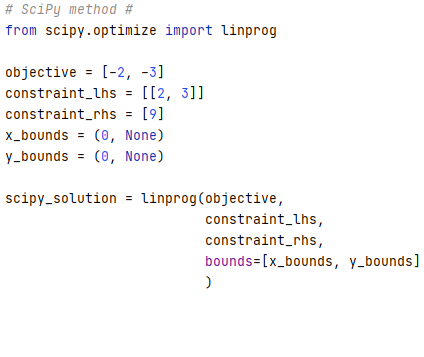
\includegraphics[height=4.8cm]{images/scipy_linprog.png}
    \end{minipage}}
    \fbox{\begin{minipage}{0.45\textwidth}
        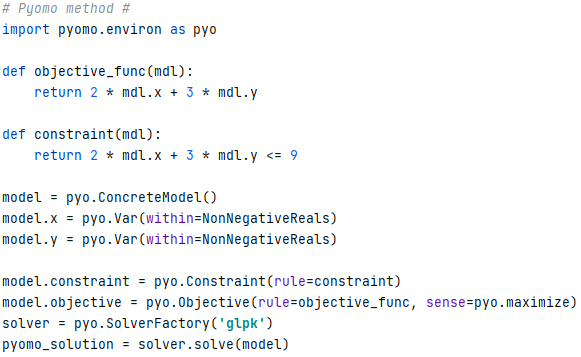
\includegraphics[height=4.8cm]{images/pyomo.png}
    \end{minipage}}
    \caption{Comparison of SciPy (left) and Pyomo (right) implementations of \cref{fig:simple_lp}}
    \label{fig:compare_lp}
\end{figure}
%TC:endignore

We also considered two libraries for visualisation: mpld3 and \acrshort{d3}.js. Mpld3 allows exporting of Matplotlib plots to \acrshort{html} . We created a basic prototype using mpld3, but we quickly found it was inflexible due to the lack of customisation for interactive legends. Furthermore for the client to render the plot in React, it would need to inject \acrshort{html} into the page which presents a potential security vulnerability. Therefore we decided to use \acrshort{d3}, a \acrshort{js} visualisation library. D3 is a more difficult library to learn since it is lower level, but it is more flexible than mpld3.
    
    \subsection{Existing Visualiser Review}\label{section:visualiser_review}
    As UX design is its own extensive field of research and visualisations were a secondary aim, we took inspiration from existing well designed visualisers TensorFlow Playground and Algorithm Visualizer.

%TC:ignore
\begin{figure}[H]
    \begin{minipage}{0.54\textwidth}
        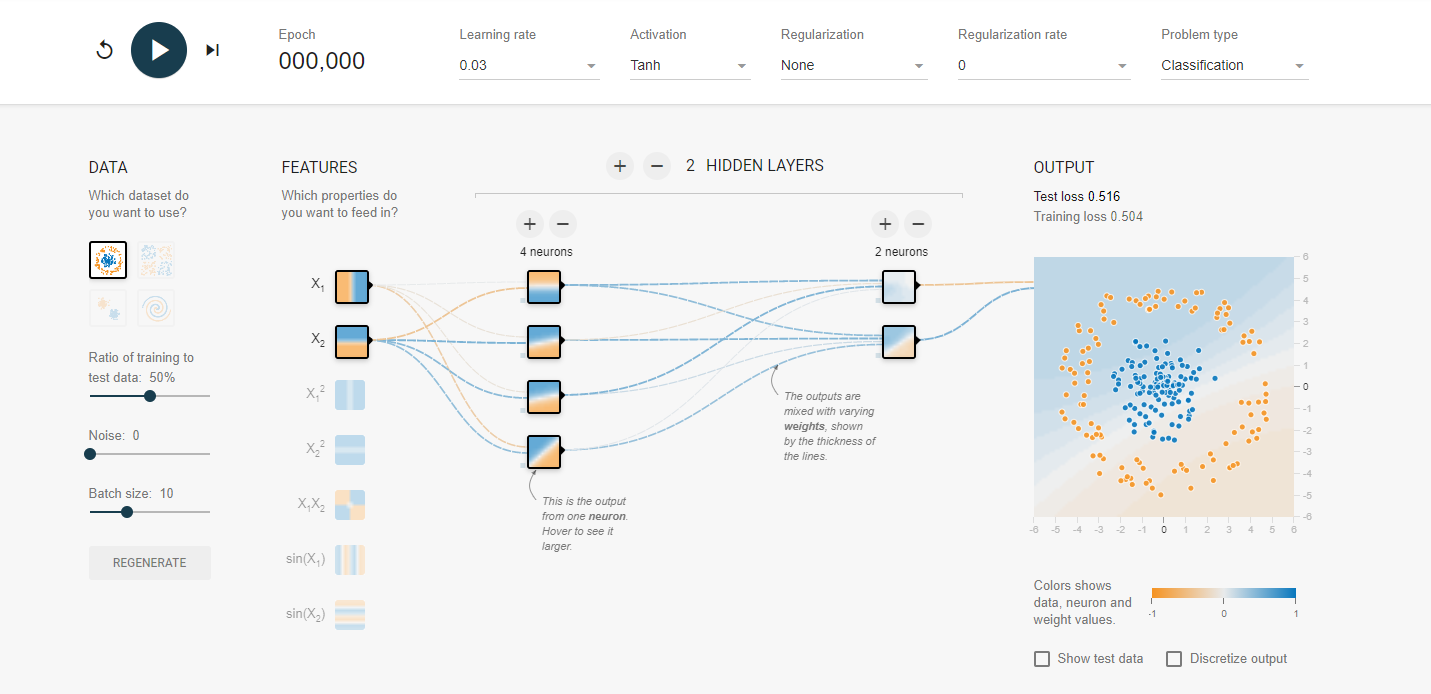
\includegraphics[height=4.3cm]{images/tensor-flow-playground.png}
        \caption{TensorFlow Playground}
        \label{fig:tensorflow_playground}
    \end{minipage}
    \begin{minipage}{0.46\textwidth}
        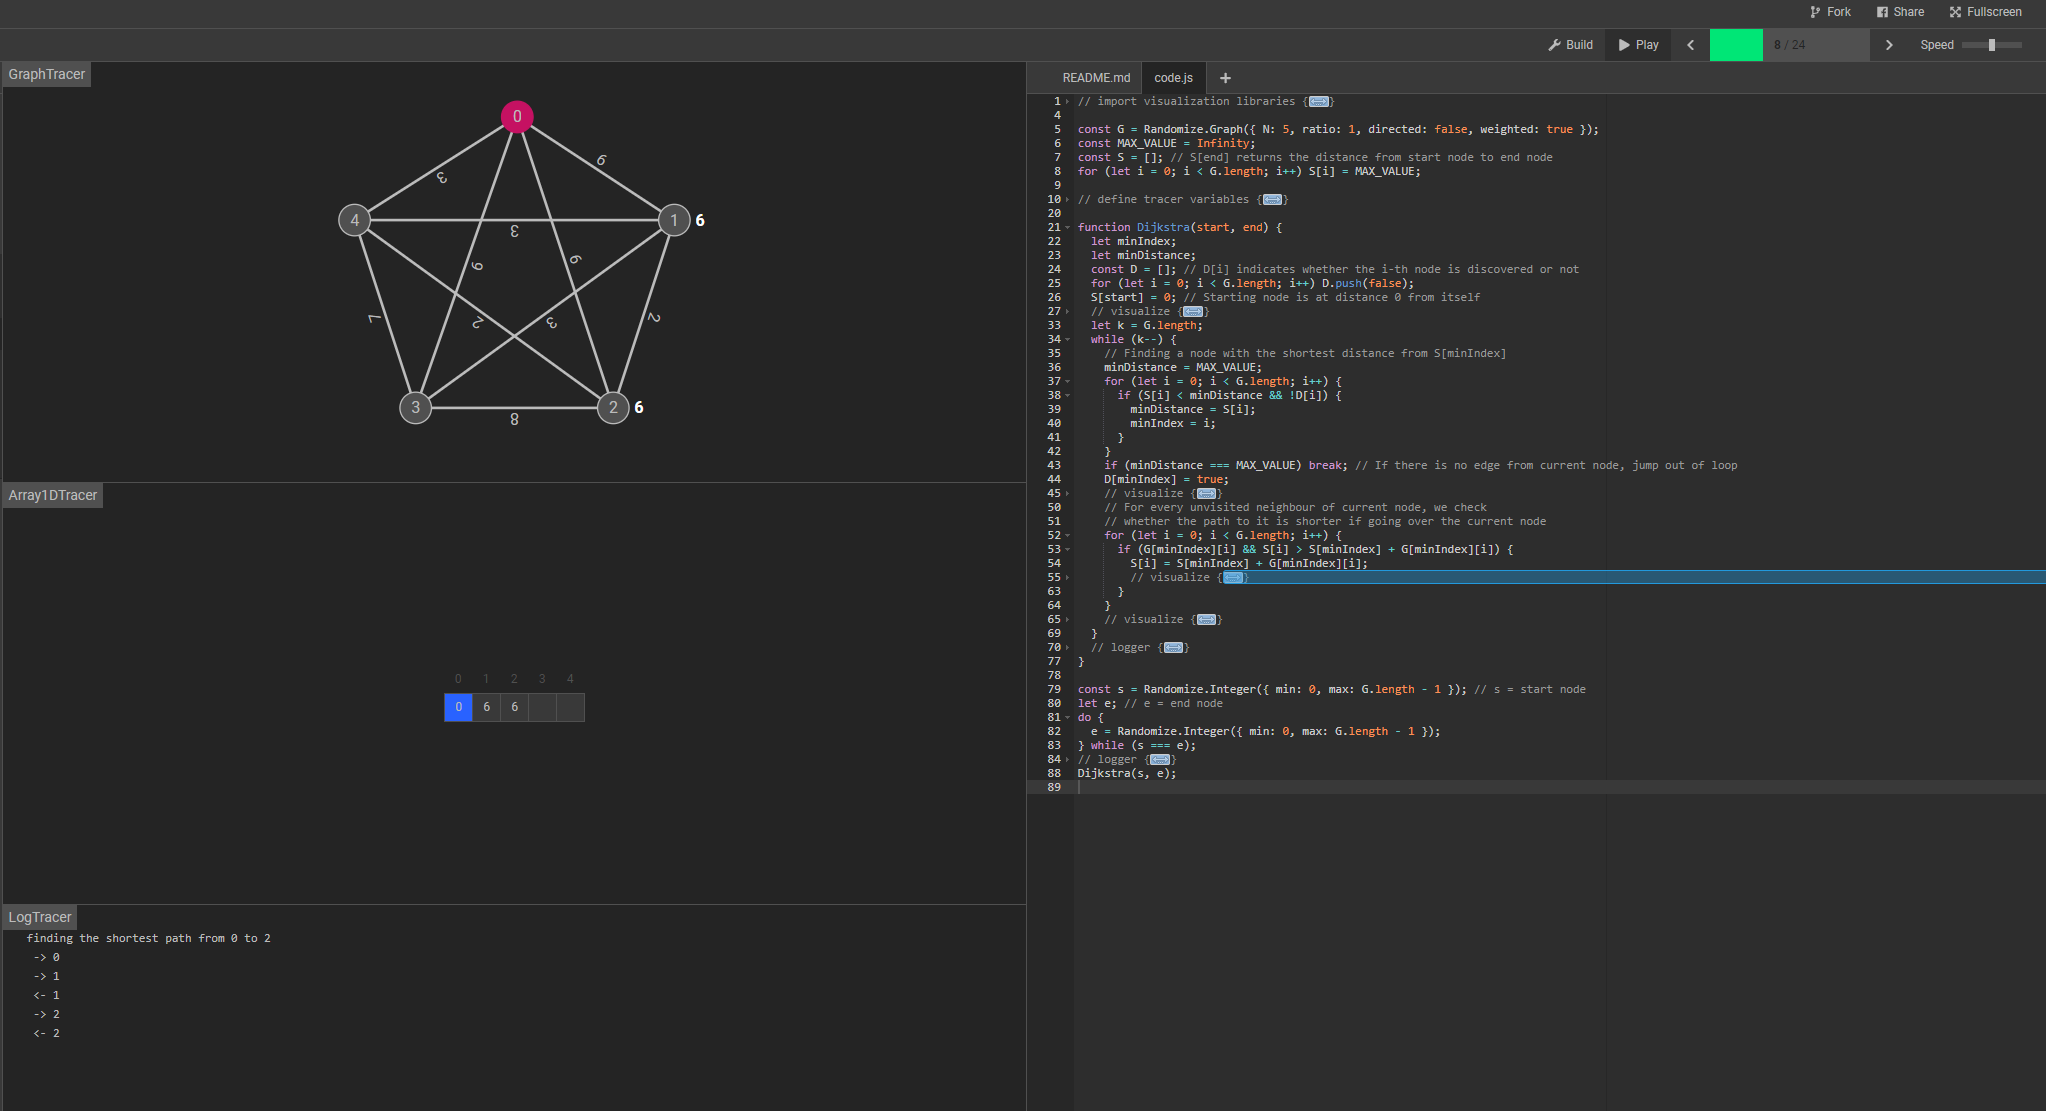
\includegraphics[height=4.3cm]{images/algorithm-visualizer.png}
        \caption{Algorithm Visualizer}
        \label{fig:algorithm_visualizer}
    \end{minipage}
\end{figure}
%TC:endignore

The key features that make both of them effective are separated panels for configuration, graphs and information. Furthermore TensorFlow playground has tooltips giving information for unlabeled components. Algorithm Visualizer allows the user to step back and forth between an algorithm. They both have a degree of interactivity, allowing users to change the input parameters to the problem.

To keep our functionality focused, we decided to separate the solution visualisation (\cref{section:solution_visualisation}) and interactive algorithm visualisation (\cref{section:stepped_visualisation}) components into seperate pages.
    
    \subsection{Solution Visualisation}\label{section:solution_visualisation}
    The solver \acrshort{ui} (\cref{fig:sol_vis}) focuses on allowing the user to compare the solutions to Colourful $k$-center problems using different algorithms. We divide the \acrshort{ui} into three columns: configuration, solution visualisation and information. 

%TC:ignore
\begin{figure}[H]
    \centering
    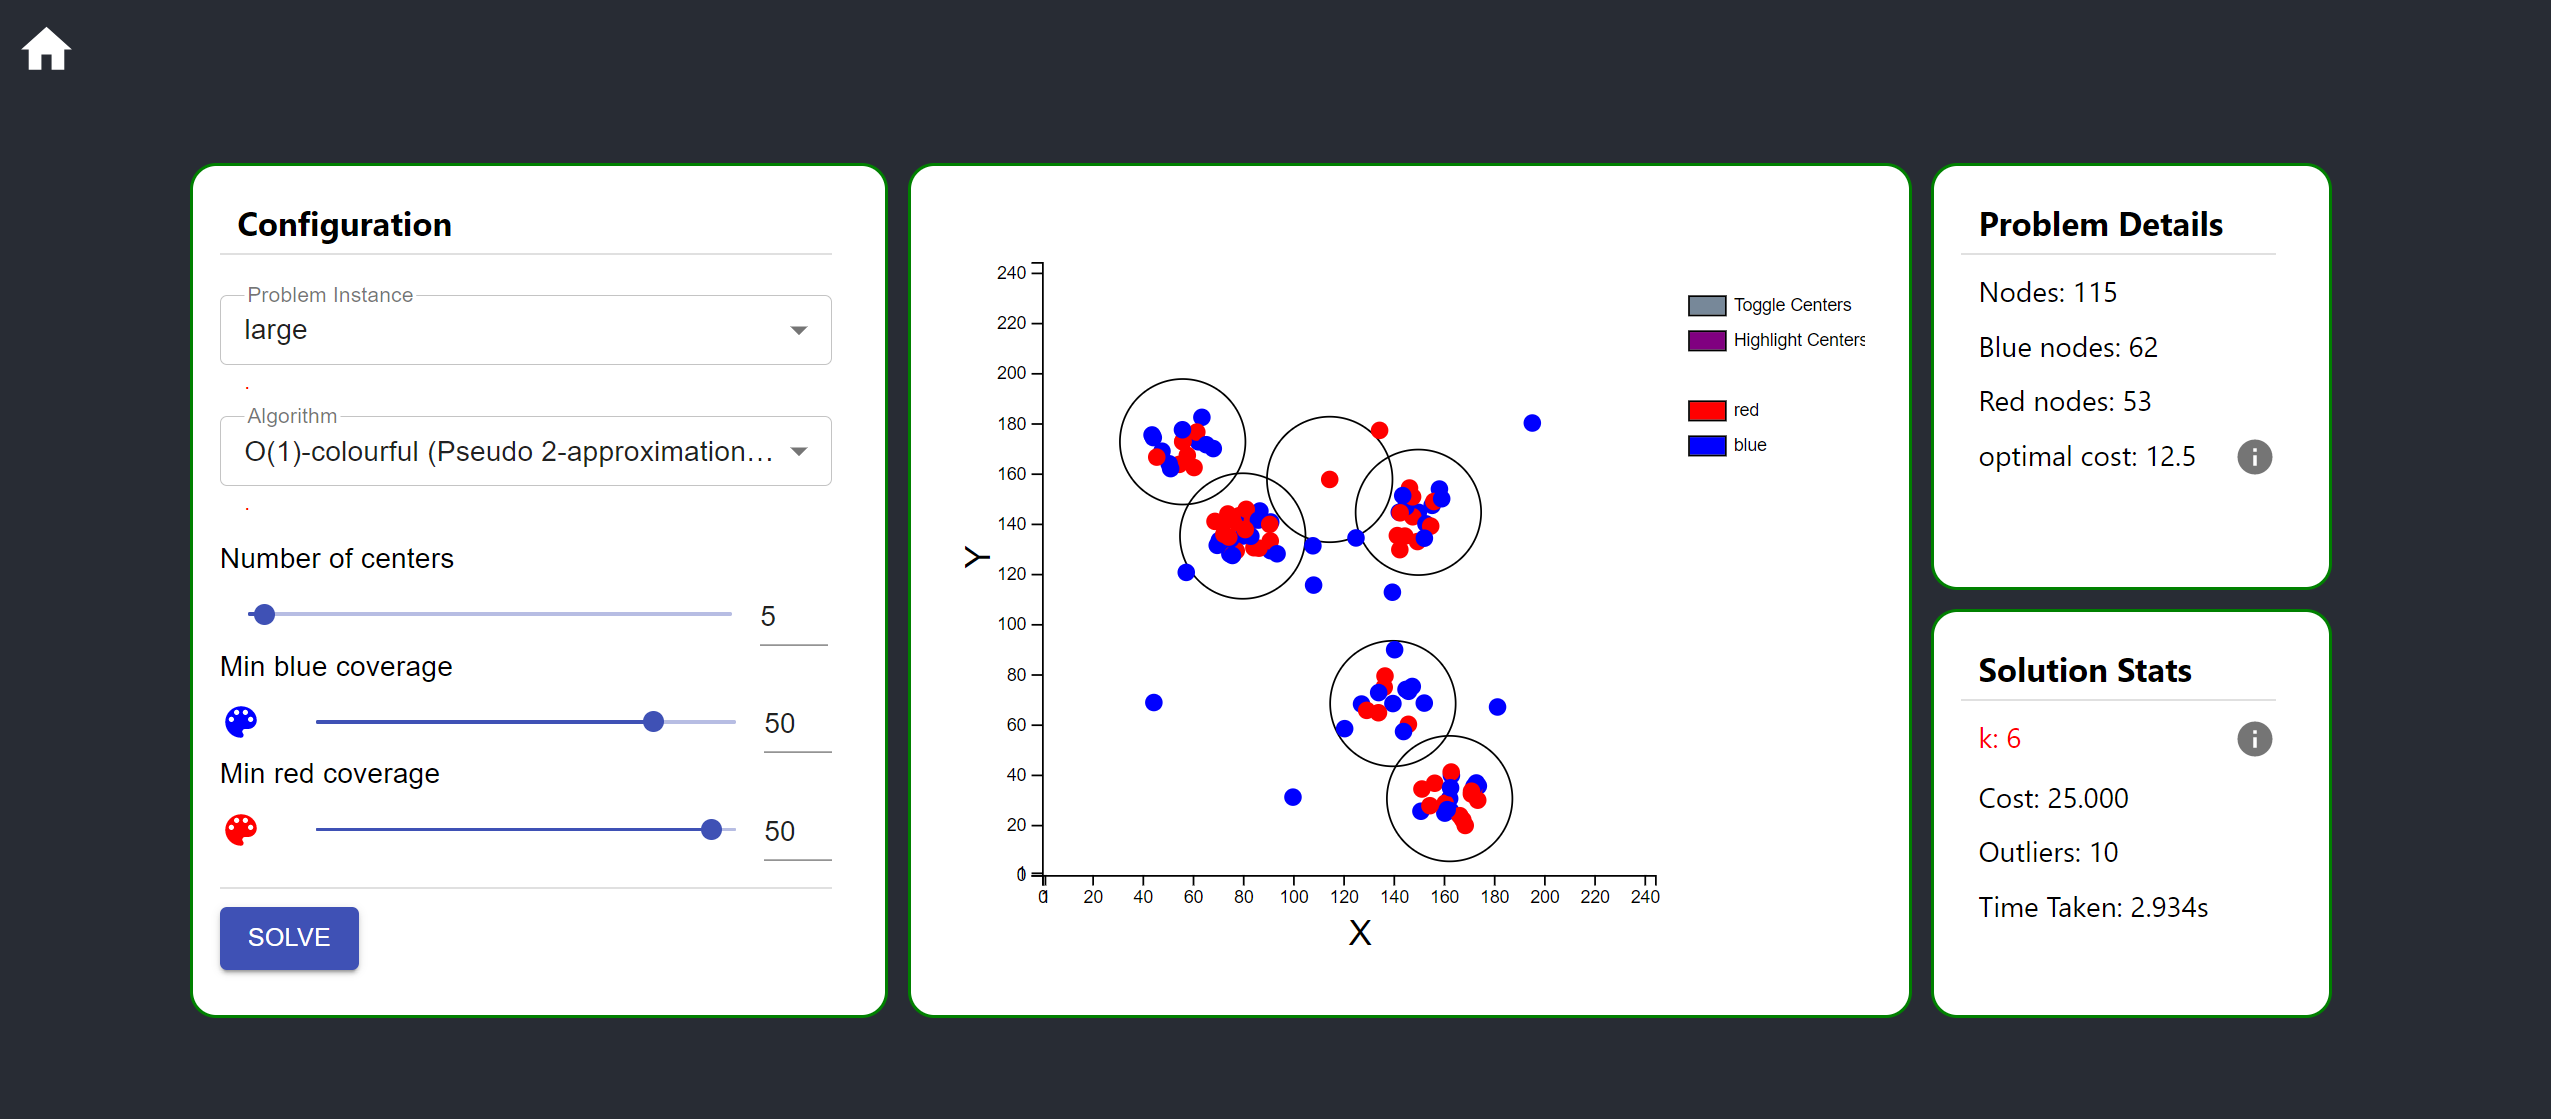
\includegraphics[width=\textwidth]{images/solver_ui/colourful_solve_zoom.png}
    \caption{Solver \acrshort{ui}\\\url{https://colourful-k-center.herokuapp.com/solve}}
    \label{fig:sol_vis}
\end{figure}
%TC:endignore

The configuration column allows the user to choose the problem, algorithm and to adjust the constraints. The visualisation column plots all vertices (colour coded), displaying the coverage generated by a solution. In addition there is an interactive legend which allow users to toggle the displayed data. Finally, the information column displays information about the problem and information about the solution. We use tooltips throughout our \acrshort{ui} to provide additional context.
    
    \subsection{Stepped Visualisation}\label{section:stepped_visualisation}
    The focus of the stepped solver is helping a user understand how each algorithm reaches a solution. Therefore we move the configuration panel to a modal window (\cref{fig:step_sol_modal}) to make room for a new panel to describe each step of the algorithm.

%TC:ignore
\begin{figure}[H]
    \centering
    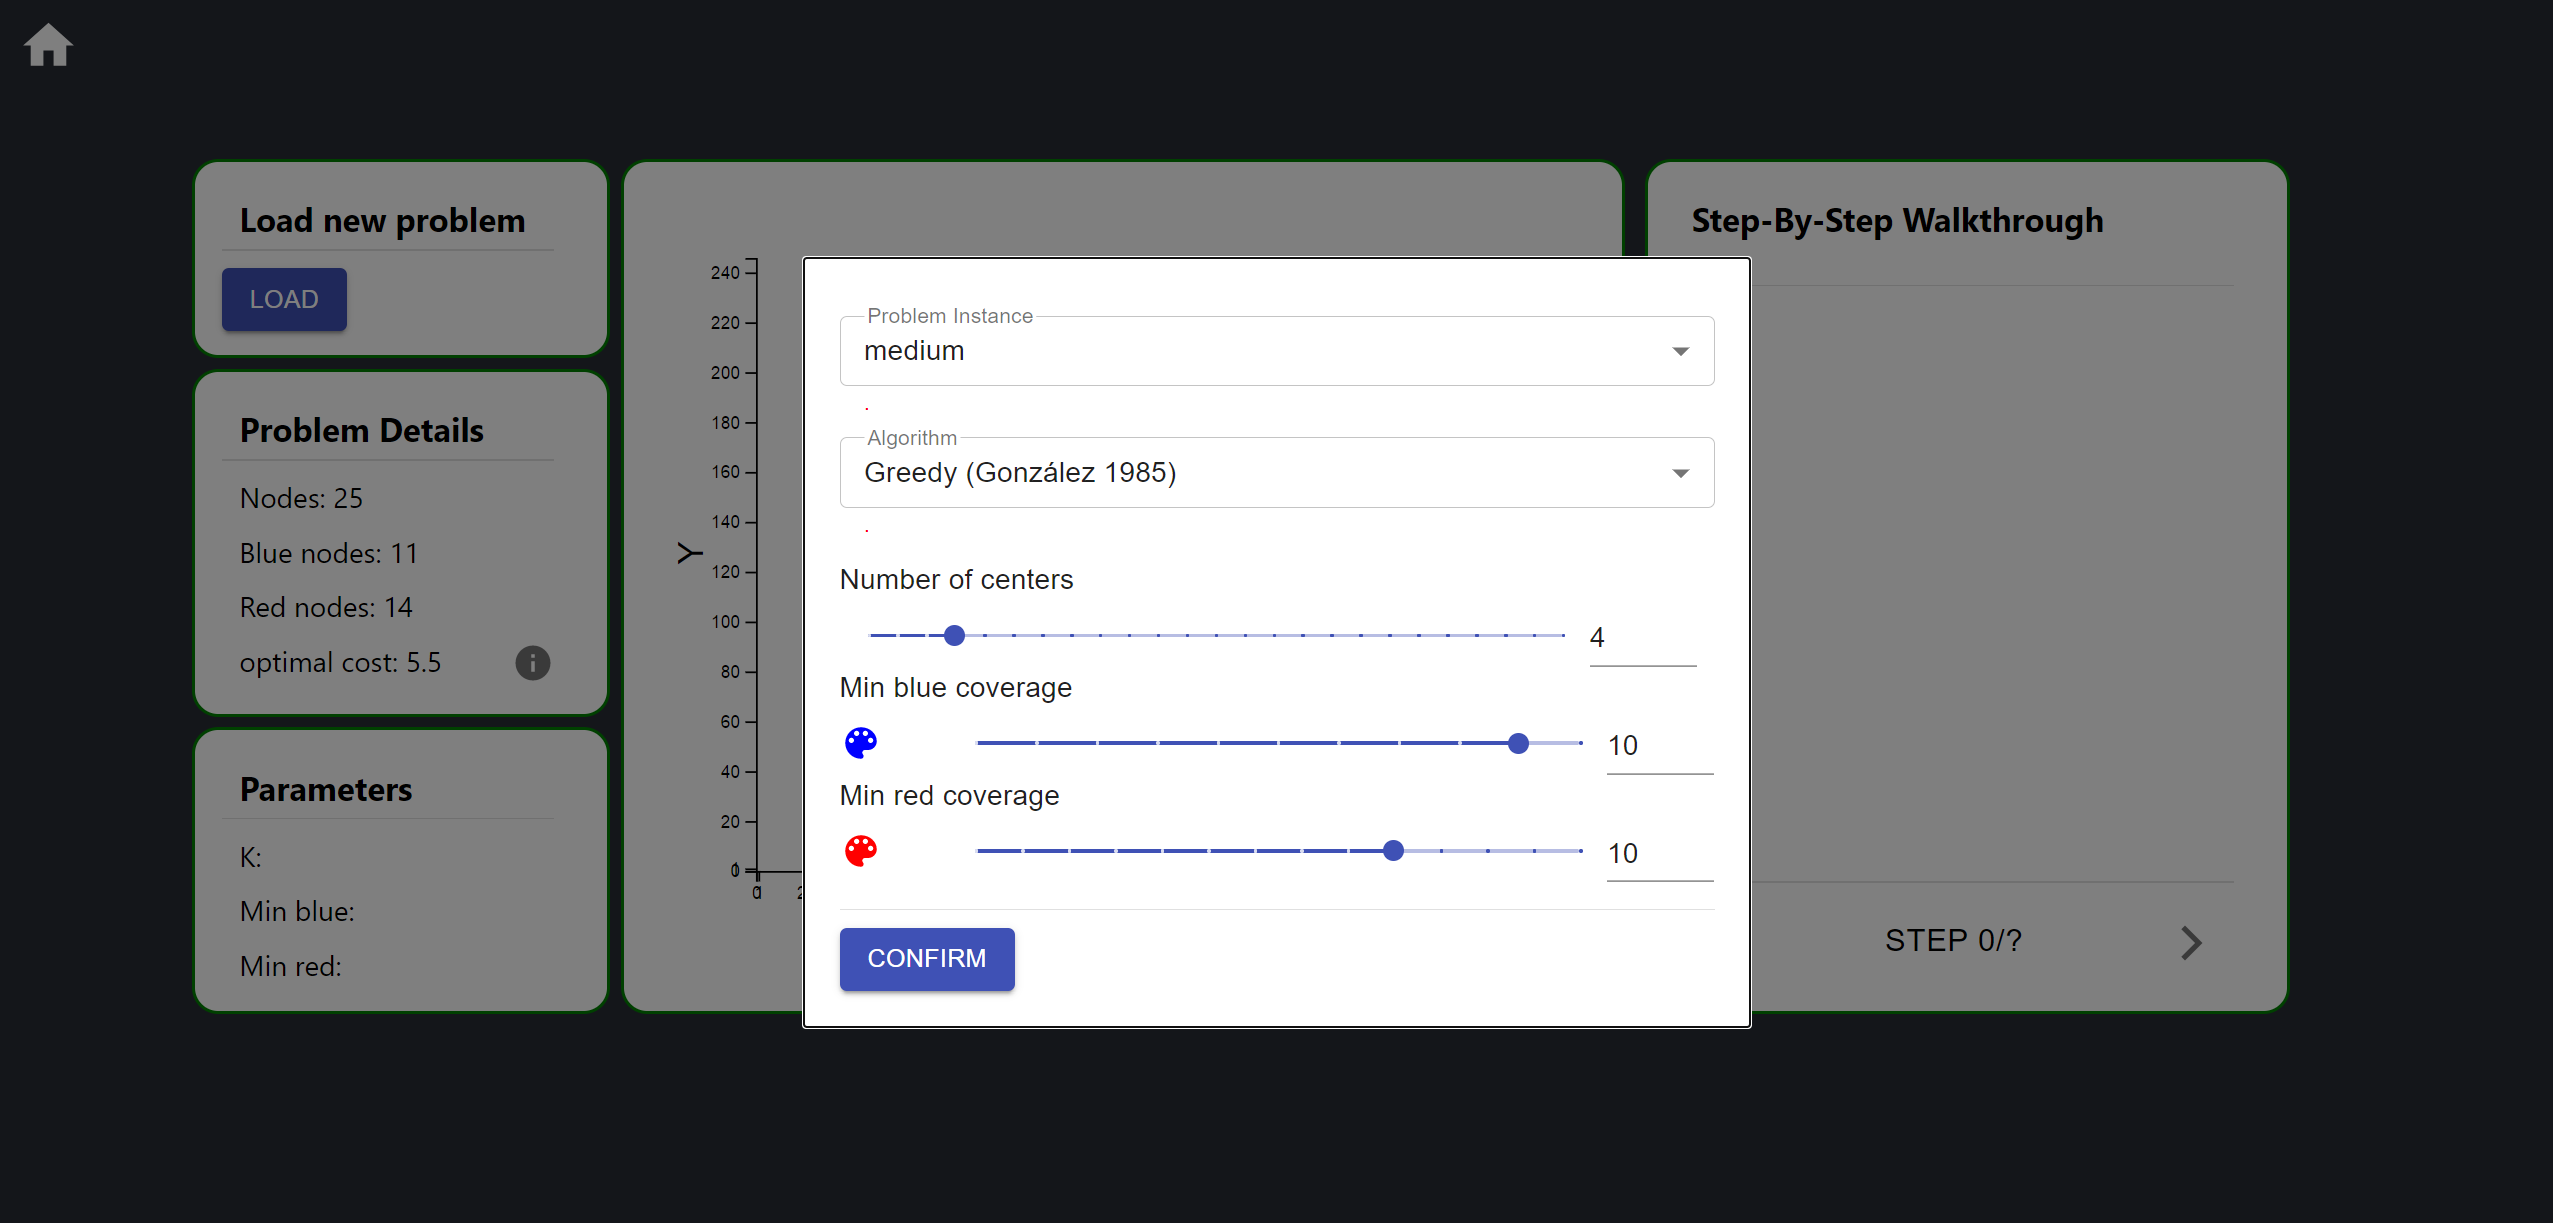
\includegraphics[width=0.7\textwidth]{images/stepped_solver_ui/stepped_solver_modal.png}
    \caption{Stepped Visualisation (configuration modal)\\\url{https://colourful-k-center.herokuapp.com/steps}}
    \label{fig:step_sol_modal}
\end{figure}
%TC:endignore

%TC:ignore
\begin{figure}[H]
    \centering
    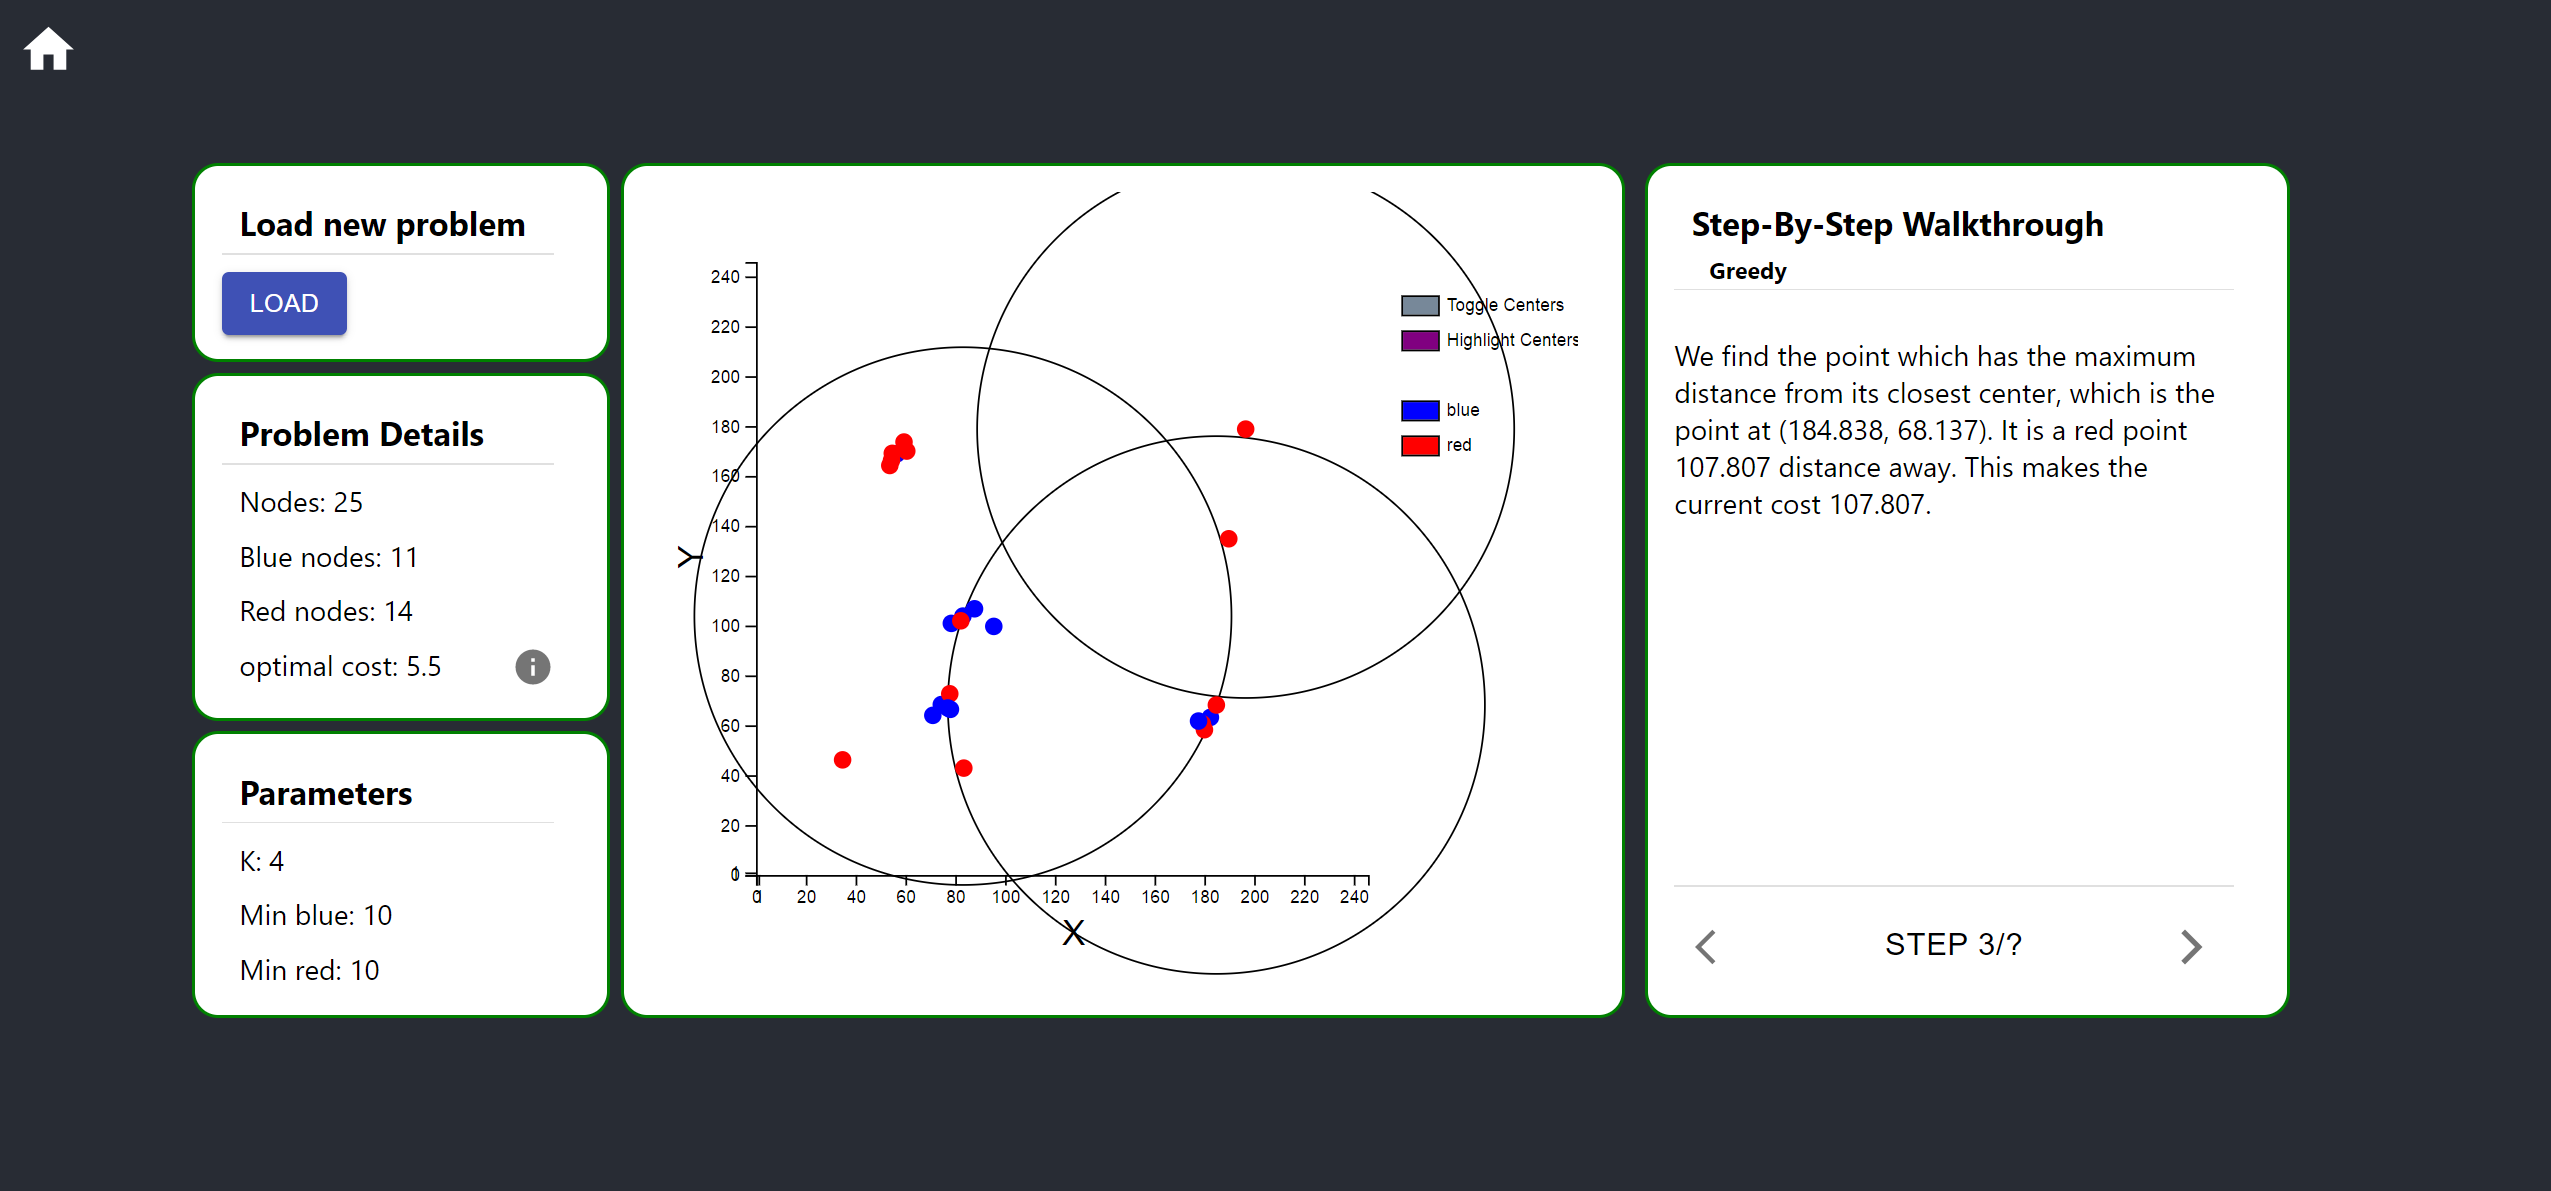
\includegraphics[width=\textwidth]{images/stepped_solver_ui/stepped_solver_greedy.png}
    \caption{Stepped Visualisation\\\url{https://colourful-k-center.herokuapp.com/steps}}
    \label{fig:step_sol_greedy}
\end{figure}
%TC:endignore

Some features of the UI have already been described in \cref{section:solution_visualisation}, therefore we will focus on the differences. We add a walk-through panel (rightmost panel, \cref{fig:step_sol_greedy}) which gives a text description of what an algorithm is doing at the current step. The previous and forward buttons allow the user to traverse the history of algorithm execution on a problem instance. The forward button requests the next step from the server, the exact logic is shown in \cref{fig:step_sol_logic}.

%TC:ignore
\begin{figure}[H]
    \centering
    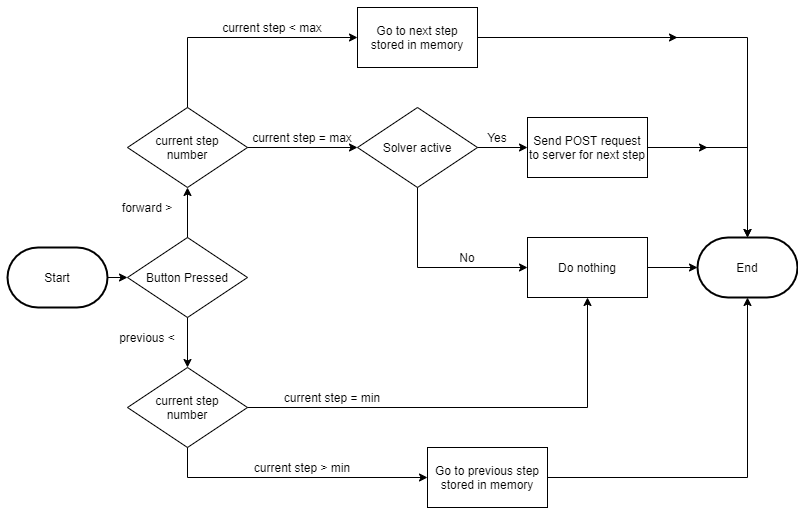
\includegraphics[width=0.85\textwidth]{images/stepped_solver_ui/walkthrough_flow.png}
    \caption{Stepped Visualisation Flow (client side)}
    \label{fig:step_sol_logic}
\end{figure}
%TC:endignore

We make considerations for visualising genetic algorithms (\acrshort{ga}s) since they have multiple solutions at each step. For a \acrshort{ga}, we design a switchable \acrshort{ui}, to show the whole population and a specific individual in the population (\cref{fig:step_sol_toggle}). 

%TC:ignore
\begin{figure}[H]
    \centering
    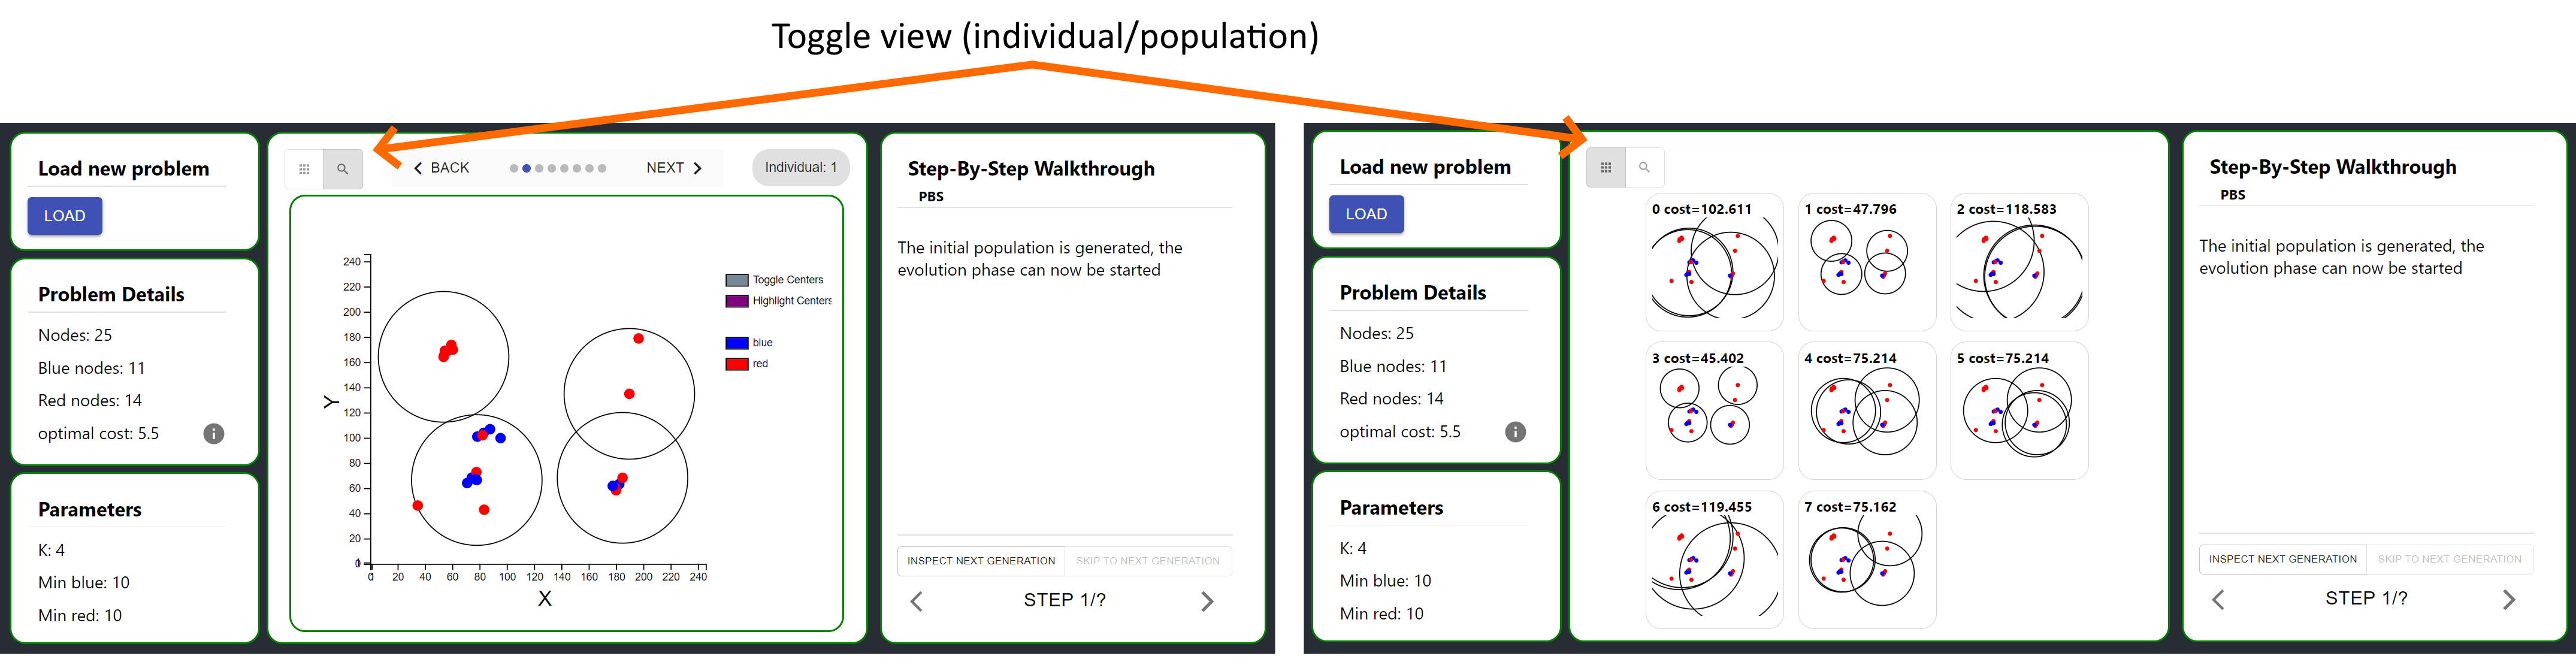
\includegraphics[width=\textwidth]{images/stepped_solver_ui/stepped_solver_toggle.png}
    \caption{View toggling for genetic algorithms}
    \label{fig:step_sol_toggle}
\end{figure}
%TC:endignore

We also consider the large number of steps in \acrshort{ga}s, therefore add an extra control bar to view all intermediate steps or to skip to the next generation (\cref{fig:step_sol_skip}).

%TC:ignore
\begin{figure}[H]
    \centering
    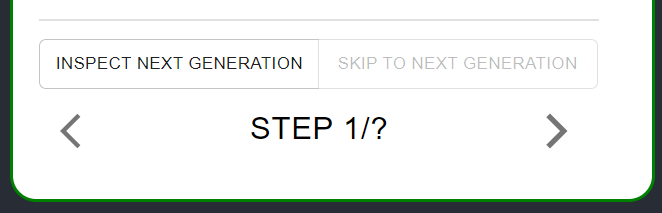
\includegraphics[width=0.35\textwidth]{images/stepped_solver_ui/stepped_solver_skip.png}
    \caption{Additional controls for genetic algorithms (walk-through panel)}
    \label{fig:step_sol_skip}
\end{figure}
%TC:endignore
    
    \subsection{Architecture}\label{section:architecture}
    %TC:ignore
\begin{figure}[H]
    \centering
    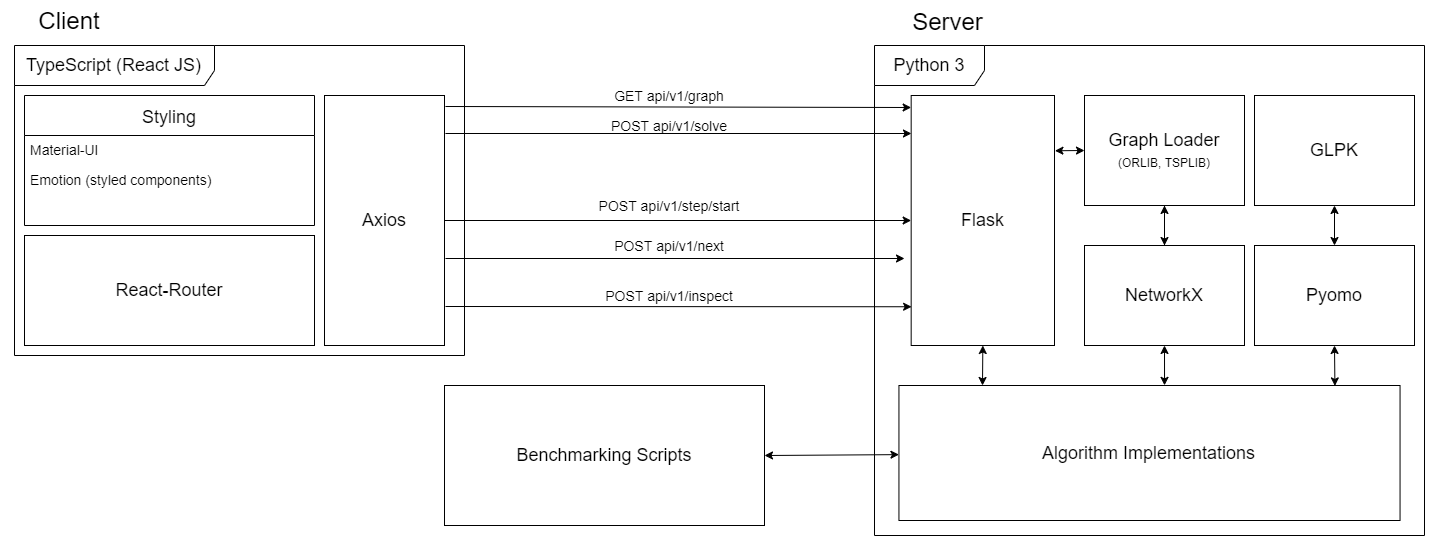
\includegraphics[width=\textwidth]{images/system_architecture.png}
    \caption{System Architecture}
    \label{fig:system_architecture}
\end{figure}
%TC:endignore

\subsubsection{Solver Flow}
The solution visualisation flow contains a single request:
%TC:ignore
\begin{figure}[H]
    \centering
    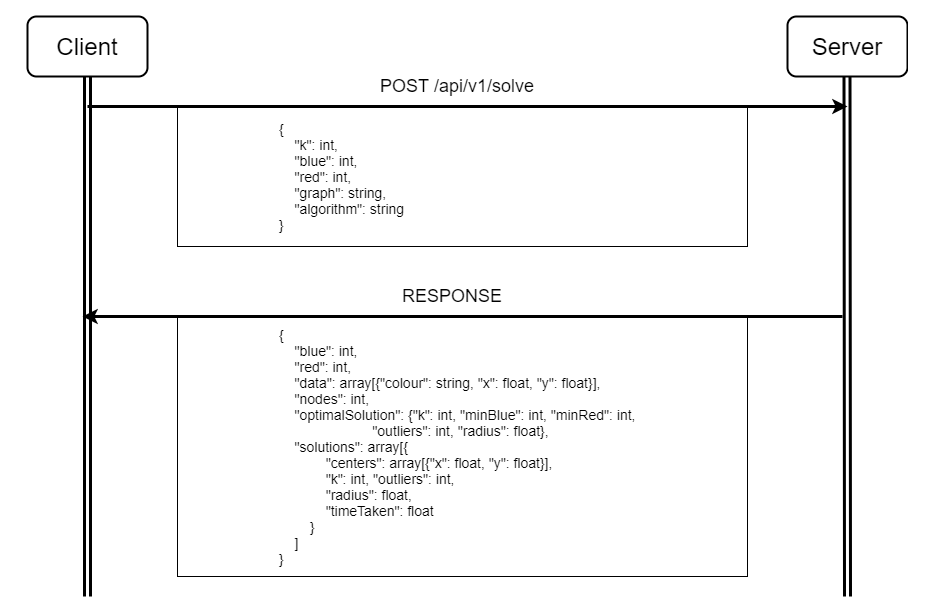
\includegraphics[width=0.85\textwidth]{images/solver_ui/post_solve_flow.png}
    \caption{Solve Request}
    \label{fig:solve_request}
\end{figure}
%TC:endignore

\subsubsection{Stepped Solver Flow}
The stepped solver is a multi request flow; it is initialised through the '/start' endpoint which creates a solver iterator and returns a \acrshort{uuid} token. The solver iterator (response, \cref{fig:stepped_next_inspect_request}) is implemented using a Python generator function which allows us to use lazy evaluation to execute the next step in the algorithm only when needed.
%TC:ignore
\begin{figure}[H]
    \centering
    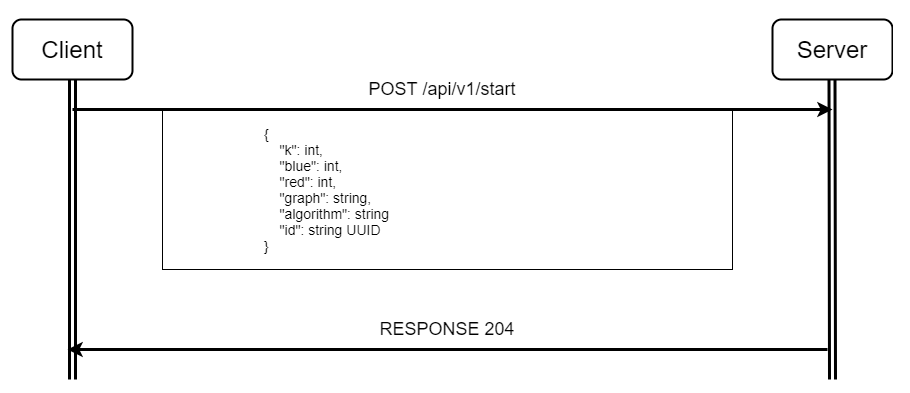
\includegraphics[width=0.8\textwidth]{images/stepped_solver_ui/start_stepped_flow.png}
    \caption{/api/v1/start flow}
    \label{fig:stepped_start_request}
\end{figure}
%TC:endignore

Subsequent calls to the '/next' and '/inspect' endpoints with the UUID is used to exhaust the iterator. Inspect moves to the next chronological step and next skips to the next major step.
%TC:ignore
\begin{figure}[H]
    \centering
    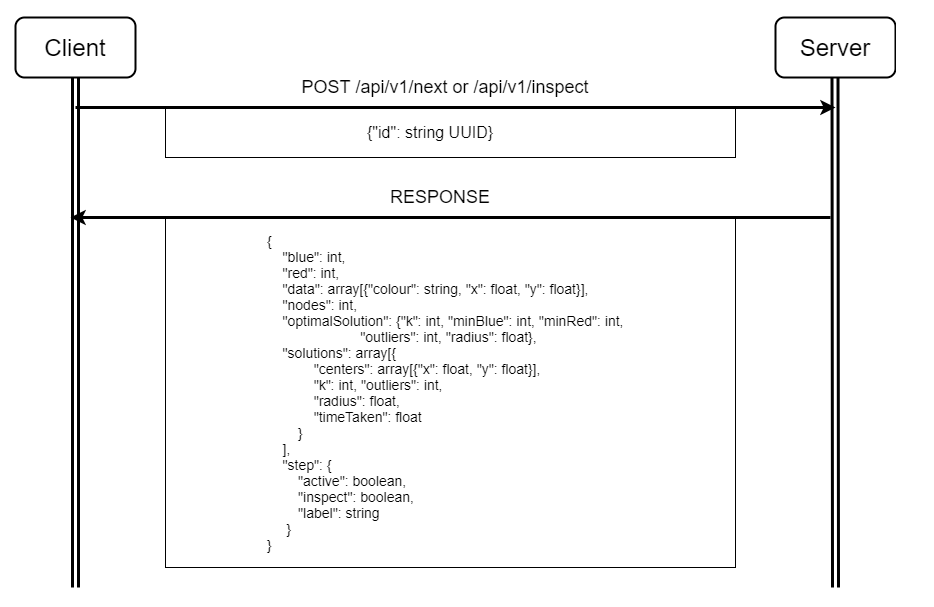
\includegraphics[width=0.8\textwidth]{images/stepped_solver_ui/next_inspect_stepped_flow.png}
    \caption{/api/v1/next and /api/v1/inspect flow}
    \label{fig:stepped_next_inspect_request}
\end{figure}
%TC:endignore

%\subsubsection{Build and Deployment}
%Following the accessibility requirement, we also consider the ease of setup. As we use linear program solvers, this is an extra dependency that is not installable the dependency manager Python pip. Therefore we use Docker, we configure the build file to create and package the static web files, install all dependencies; a user can clone our git repository, execute 'docker build' and 'docker run', then have a working instance of our application. This also allows us to easily deploy to cloud platforms such as Heroku.

\section{Results}\label{section:results}
    \subsection{Methodology}\label{section:methodology}
    We conduct empirical experiments to evaluate the performance of each algorithm. \acrshort{grasp_ps}, \acrshort{pbs} and colourful PBS are stochastic and therefore have a degree of variability in solution cost. In the context of genetic algorithms, \textcite{kramer_genetic_2017} suggests that 50 trials is sufficient to address variance. We set a timeout for the $k$-center algorithms to $0.1n + 0.5k$ seconds and $0.15n + 0.5k$ for the colourful $k$-center algorithms (since it is harder). When benchmarking the \emph{Ban} algorithm, if it returned more than $k$-centers, we retried the test with $k-1$ as the parameter. For algorithms that produce multiple results (such as colourful PBS) we record the time at which the minimum cost is reached. All experiments were conducted on an AMD 4.2GHz Ryzen 4800h PC with 16gb ram. 

\paragraph{Data Sets}~\\
To evaluate the algorithms for the $k$-center we use the OR-LIB dataset (\cite{beasley_note_1985}), originally designed for the $k$-median but later widely used for the $k$-center. OR-LIB has 40 problem instances ranging from 100-900 nodes with known optimal solutions (\cite{pullan_memetic_2008}). 

As the colourful $k$-center problem was introduced very recently, it does not have any data sets. Generating our own data sets raises two issues; there may be bias in our data generation method and we may not know the optimal solution to our instances. Therefore we create two new data sets to address this (see \cref{appendix:test_datasets}):
\begin{enumerate}
    \item GOWALLA - To address the possibility of bias in synthetic data sets, we used a real world 3D data set. We take inspiration from the Gowalla UCI Repeat Consumption Matrices (\cite{kotzias_predicting_2019}), which is based on the number of times a user has checked in at a location. The UCI data set uses discretised geolocations, as this information is important to our problem we generate our own repeat consumption matrices (with latitude/longitude information) from the original Gowalla data set (\cite{cho_friendship_2011}). The locations can be split into blue/red by setting locations visited less frequently than average as blue and more frequently as red. The distance between two locations is defined by the Haversine distance. 
    \item SYNTHETIC - 40 problems of 100-900 nodes in a 2D plane with known optimal costs (\emph{opt}). Given an optimal cost $\rho$ and $k$, we generate $k$ centers, a uniform random set of inlier points $\leq\rho$ distance from a center, and a set of outlier points $>\rho$ from the centers. We generate 36 instances with 20\% of the vertices as outliers and 4 problem instances which have 80\% of vertices as outliers. The full procedure is described in \cref{appendix:generate_problem_instances}.
\end{enumerate}

\paragraph{Statistical Analysis Methods}~\\
To decide whether our results are significant we perform statistical tests. The null hypothesis is that the results come from the same distribution. The statistical test outputs a p-value, in order to reject the null hypothesis the p-value needs to fall below a significance level $\alpha$. We take $\alpha =0.05$, which means there is a 5\% risk of concluding our samples come from different distributions when they are not. We perform the Wilcoxon test for the colourful $k$-center and the Quade test for the $k$-center.

\newcounter{method_counter}
\setcounter{method_counter}{0}
\begin{figure}[H] 
    \addtocounter{figure}{-1}
    \renewcommand{\thefigure}{\arabic{method_counter}}
    \renewcommand\figurename{Method}
    \addtocounter{method_counter}{1}
    \caption{Wilcoxon (\cite{wilcoxon_individual_1945})}
    \label{method:wilcoxon_test}
    \vspace{0.1cm}
    \textbox{\small{\textbf{Wilcoxon signed rank test}\newline A statistical hypothesis test for two sets of paired samples. The general idea is to calculate the differences between pairs then rank the differences by size. The test statistic is calculated by summing the ranks multiplied by the sign of the differences.\newline \textbf{R function: wilcoxon.test(sampleA, sampleB, paired=true)}}}
\end{figure}

\begin{figure}[H] 
    \addtocounter{figure}{-1}
    \renewcommand{\thefigure}{\arabic{method_counter}}
    \renewcommand\figurename{Method}
    \addtocounter{method_counter}{1}
    \caption{Quade (\cite{conover_analysis_1982})}
    \label{method:quade_test}
    \vspace{0.1cm}
    \textbox{\small{\textbf{Quade omnibus test}\newline An extension of the Wilcoxon test for 3 or more sets of grouped samples. An omnibus test is used to determine if the variance between all samples are significant.\newline \textbf{R function: quade.test(matrix)}}}
\end{figure}

\begin{figure}[H] 
    \addtocounter{figure}{-1}
    \renewcommand{\thefigure}{\arabic{method_counter}}
    \renewcommand\figurename{Method}
    \addtocounter{method_counter}{1}
    \caption{Post-Hoc Quade (\cite{conover_analysis_1982})}
    \label{method:post_hoc_quade}
    \vspace{0.1cm}
    \textbox{\small{\textbf{Post-hoc Quade test}\newline If the Quade omnibus test returns a significant result we would like to determine which pairs of samples are significant. This is done using a post-hoc test, which returns p-values for each paired sample. \newline\textbf{R function: quadeAllPairsTest(matrix, dist="TDist", p.adjust.method="holm")}}}
\end{figure}

Given our results are statistically significant, we count the number of problem instances where one algorithm outperforms another to determine the better algorithm. 

\begin{figure}[H] 
    \addtocounter{figure}{-1}
    \renewcommand{\thefigure}{\arabic{method_counter}}
    \renewcommand\figurename{Method}
    \addtocounter{method_counter}{1}
    \caption{Counting results}
    \label{method:counting_results}
    \vspace{0.1cm}
    \textbox{\small{Given paired samples A and B, we count the number of problem instances where A has a lower mean cost ($\mu$) than B. If more than half of the problem instances have lower cost in sample A than B and a statistical test proves that the difference is significant, then we conclude A is better than B.}}
\end{figure}

\begin{figure}[H] 
    \addtocounter{figure}{-1}
    \renewcommand{\thefigure}{\arabic{method_counter}}
    \renewcommand\figurename{Method}
    \addtocounter{method_counter}{1}
    \caption{Counting results (accounting for variance)}
    \label{method:counting_results_variance}
    \vspace{0.1cm}
    \textbox{\small{We use the \gls{empirical_rule} to account to account for variance, it states that under a normal distribution under a normal distribution 95\% and 99.7\% of data will fall under 2 and 3 standard deviations from the mean respectively. We use the same method as \Cref{method:counting_results}, except we adjust the mean costs ($\mu$) by a parameter $\Delta\in\{2,3\}$ which represents the number of standard deviations. We increase the mean costs from sample A by $\Delta\sigma$ and modify the costs from sample B to be $max(opt, B_i -\Delta\sigma)$, $i\in$ problem\_instances (if $opt$ is unknown, set the cost to $B_i -\Delta\sigma$).\newline\newline If more than half of the problem instances have lower cost in sample A than B and a statistical test proves that the difference is significant, then we conclude A is better than B.}}
\end{figure}

\begin{table}[H]
    \centering
    \small
    \begin{tabular}{lccccc}
        \firsthline
         \textbf{Algorithm} &  1 (Wilcoxon) & 2 (Quade) &  3 (Post-hoc Quade) & 4 (Counting) & 5 (Empirical Rule)\\
         \hline
         Gon & & \checkmark & \checkmark & \checkmark & \checkmark\\
         PBS & & \checkmark & \checkmark & \checkmark & \checkmark\\
         GRASP-PS & & \checkmark & \checkmark & \checkmark & \checkmark\\
         Ban & \checkmark & & & \checkmark & \checkmark\\
         Colourful PBS & \checkmark & & & \checkmark & \checkmark\\
        \lasthline
    \end{tabular}
    \caption{Summary of methods used in analysis}
    \label{tab:method used}
    \normalsize
\end{table}
    
    \subsection{\texorpdfstring{$k$}{k}-center ORLIB}\label{section:k_center_orlib}
    %TC:ignore
\begin{table}[H]
    \caption{Results on ORLIB instances}\label{table:orlib_cost}
    \tiny
    \begin{tabularx}{\textwidth}{XXlXXXXlXXXXlXXXX}
    \firsthline
    \multicolumn{2}{c}{Instance}& \quad & \multicolumn{4}{c}{gon}& \quad & \multicolumn{4}{c}{grasp}& \quad & \multicolumn{4}{c}{pbs}\\
    \cline{1-2} \cline{4-7} \cline{9-12} \cline{14-17}\\
    name & opt && min & $\mu$ & $\sigma$ & \%-gap (opt) && min & $\mu$ & $\sigma$ & \%-gap (opt) && min & $\mu$ & $\sigma$ & \%-gap (opt)\\
    \hline
    pmed1 & 127.00 && 186.00 & 186.00 & 0.00 & 46.00 && 127.00 & 127.34 & 0.68 & 0.00 && 127.00 & 127.00 & 0.00 & 0.00\\
    pmed2 & 98.00 && 131.00 & 131.00 & 0.00 & 34.00 && 102.00 & 106.38 & 2.01 & 9.00 && 98.00 & 98.00 & 0.00 & 0.00\\
    pmed3 & 93.00 && 154.00 & 154.00 & 0.00 & 66.00 && 96.00 & 101.90 & 1.63 & 10.00 && 94.00 & 94.00 & 0.00 & 1.00\\
    pmed4 & 74.00 && 114.00 & 114.00 & 0.00 & 54.00 && 84.00 & 87.10 & 2.51 & 18.00 && 79.00 & 79.00 & 0.00 & 7.00\\
    pmed5 & 48.00 && 71.00 & 71.00 & 0.00 & 48.00 && 59.00 & 63.28 & 1.96 & 32.00 && 50.00 & 52.18 & 0.91 & 9.00\\
    pmed6 & 84.00 && 138.00 & 138.00 & 0.00 & 64.00 && 85.00 & 87.56 & 1.77 & 4.00 && 84.00 & 84.00 & 0.00 & 0.00\\
    pmed7 & 64.00 && 96.00 & 96.00 & 0.00 & 50.00 && 69.00 & 73.48 & 1.53 & 15.00 && 64.00 & 64.00 & 0.00 & 0.00\\
    pmed8 & 55.00 && 81.00 & 81.00 & 0.00 & 47.00 && 67.00 & 69.68 & 1.33 & 27.00 && 58.00 & 58.00 & 0.00 & 5.00\\
    pmed9 & 37.00 && 57.00 & 57.00 & 0.00 & 54.00 && 50.00 & 55.00 & 2.01 & 49.00 && 56.00 & 56.00 & 0.00 & 51.00\\
    pmed10 & 20.00 && 31.00 & 31.00 & 0.00 & 55.00 && 32.00 & 38.08 & 1.74 & 90.00 && 25.00 & 25.82 & 0.89 & 29.00\\
    pmed11 & 59.00 && 73.00 & 73.00 & 0.00 & 24.00 && 59.00 & 61.16 & 1.10 & 4.00 && 59.00 & 59.96 & 0.20 & 2.00\\
    pmed12 & 51.00 && 71.00 & 71.00 & 0.00 & 39.00 && 55.00 & 59.90 & 1.35 & 17.00 && 55.00 & 65.94 & 7.75 & 29.00\\
    pmed13 & 36.00 && 59.00 & 59.00 & 0.00 & 64.00 && 45.00 & 47.28 & 0.78 & 31.00 && 37.00 & 37.00 & 0.00 & 3.00\\
    pmed14 & 26.00 && 41.00 & 41.00 & 0.00 & 58.00 && 40.00 & 44.88 & 1.68 & 73.00 && 33.00 & 34.32 & 1.19 & 32.00\\
    pmed15 & 18.00 && 25.00 & 25.00 & 0.00 & 39.00 && 34.00 & 35.90 & 1.00 & 99.00 && 21.00 & 22.26 & 0.93 & 24.00\\
    pmed16 & 47.00 && 84.00 & 84.00 & 0.00 & 79.00 && 47.00 & 48.10 & 0.46 & 2.00 && 47.00 & 47.00 & 0.00 & 0.00\\
    pmed17 & 39.00 && 56.00 & 56.00 & 0.00 & 44.00 && 42.00 & 43.76 & 0.59 & 12.00 && 39.00 & 39.00 & 0.00 & 0.00\\
    pmed18 & 28.00 && 44.00 & 44.00 & 0.00 & 57.00 && 38.00 & 41.60 & 1.37 & 49.00 && 38.00 & 38.00 & 0.00 & 36.00\\
    pmed19 & 18.00 && 29.00 & 29.00 & 0.00 & 61.00 && 30.00 & 31.42 & 0.87 & 75.00 && 23.00 & 24.96 & 0.28 & 39.00\\
    pmed20 & 13.00 && 18.00 & 18.00 & 0.00 & 38.00 && 28.00 & 30.96 & 1.47 & 138.00 && 17.00 & 18.58 & 0.92 & 43.00\\
    pmed21 & 40.00 && 53.00 & 53.00 & 0.00 & 32.00 && 40.00 & 42.08 & 0.66 & 5.00 && 40.00 & 40.00 & 0.00 & 0.00\\
    pmed22 & 38.00 && 56.00 & 56.00 & 0.00 & 47.00 && 43.00 & 44.04 & 0.28 & 16.00 && 39.00 & 39.88 & 0.68 & 5.00\\
    pmed23 & 22.00 && 34.00 & 34.00 & 0.00 & 55.00 && 32.00 & 34.44 & 1.17 & 57.00 && 26.00 & 26.92 & 0.27 & 22.00\\
    pmed24 & 15.00 && 23.00 & 23.00 & 0.00 & 53.00 && 26.00 & 28.34 & 1.05 & 89.00 && 19.00 & 20.88 & 0.47 & 39.00\\
    pmed25 & 11.00 && 16.00 & 16.00 & 0.00 & 45.00 && 23.00 & 28.56 & 2.41 & 160.00 && 15.00 & 15.04 & 0.20 & 37.00\\
    pmed26 & 38.00 && 50.00 & 50.00 & 0.00 & 32.00 && 39.00 & 40.00 & 0.66 & 5.00 && 38.00 & 38.04 & 0.28 & 0.00\\
    pmed27 & 32.00 && 43.00 & 43.00 & 0.00 & 34.00 && 35.00 & 35.78 & 0.54 & 12.00 && 33.00 & 33.00 & 0.00 & 3.00\\
    pmed28 & 18.00 && 28.00 & 28.00 & 0.00 & 56.00 && 27.00 & 28.84 & 0.99 & 60.00 && 26.00 & 26.00 & 0.00 & 44.00\\
    pmed29 & 13.00 && 20.00 & 20.00 & 0.00 & 54.00 && 24.00 & 27.98 & 2.29 & 115.00 && 18.00 & 18.02 & 0.14 & 39.00\\
    pmed30 & 9.00 && 14.00 & 14.00 & 0.00 & 56.00 && 24.00 & 26.22 & 1.79 & 191.00 && 12.00 & 12.92 & 0.34 & 44.00\\
    pmed31 & 30.00 && 42.00 & 42.00 & 0.00 & 40.00 && 31.00 & 32.18 & 0.62 & 7.00 && 30.00 & 30.02 & 0.14 & 0.00\\
    pmed32 & 29.00 && 45.00 & 45.00 & 0.00 & 55.00 && 31.00 & 32.98 & 0.71 & 14.00 && 31.00 & 60.80 & 17.96 & 110.00\\
    pmed33 & 15.00 && 25.00 & 25.00 & 0.00 & 67.00 && 24.00 & 25.90 & 1.32 & 73.00 && 19.00 & 19.00 & 0.00 & 27.00\\
    pmed34 & 11.00 && 17.00 & 17.00 & 0.00 & 55.00 && 23.00 & 26.38 & 1.73 & 140.00 && 15.00 & 15.32 & 0.47 & 39.00\\
    pmed35 & 30.00 && 38.00 & 38.00 & 0.00 & 27.00 && 31.00 & 32.68 & 0.55 & 9.00 && 30.00 & 30.42 & 0.60 & 1.00\\
    pmed36 & 27.00 && 41.00 & 41.00 & 0.00 & 52.00 && 30.00 & 31.70 & 0.78 & 17.00 && 29.00 & 40.76 & 3.72 & 51.00\\
    pmed37 & 15.00 && 25.00 & 25.00 & 0.00 & 67.00 && 24.00 & 26.88 & 1.32 & 79.00 && 19.00 & 19.00 & 0.00 & 27.00\\
    pmed38 & 29.00 && 39.00 & 39.00 & 0.00 & 34.00 && 29.00 & 32.08 & 1.15 & 11.00 && 40.00 & 40.00 & 0.00 & 38.00\\
    pmed39 & 23.00 && 35.00 & 35.00 & 0.00 & 52.00 && 25.00 & 26.54 & 0.70 & 15.00 && 74.00 & 74.00 & 0.00 & 222.00\\
    pmed40 & 13.00 && 21.00 & 21.00 & 0.00 & 62.00 && 22.00 & 24.04 & 1.17 & 85.00 && 18.00 & 18.00 & 0.00 & 38.00\\
    \hline
    \multicolumn{2}{l}{Average} &&&&& 49.87 &&&&& 47.83 &&&&& 27.38\\
    \hline
    \multicolumn{4}{r}{Quade test on mean costs} & \multicolumn{3}{l}{p-value=\num{7.25e-9}} & \multicolumn{10}{c}{}\\
    \lasthline
    \end{tabularx}
    \normalsize
\end{table}
%TC:endignore

\paragraph{Analysis of solution cost}~\\
The Quade omnibus test on the $\mu$ costs (\cref{table:orlib_cost}) returned a p-value of \num{7.25e-9}. As the omnibus test returned a statistically significant result, we perform a post-hoc Quade test to determine whether the pairwise difference between the three algorithms are significant (\cref{table:post_hoc_orlib}).

%TC:ignore
\begin{table}[H]
    \centering
    \caption{P-values from post-hoc Quade test on ORLIB $\mu$ costs}\label{table:post_hoc_orlib}
    \begin{tabularx}{0.75\textwidth}{|X|XX|}
        \hline
        \textbf{Algorithm} & \emph{Gon} & GRASP Plateau Surfer\\
        \hline
        GRASP Plateau Surfer & \num{4.14e-3} & N/A\\
        PBS & \num{3.46e-9} & \num{3.30e-4}\\
        \lasthline
    \end{tabularx}
\end{table}
%TC:endignore

%TC:ignore
\begin{figure}[H]
    \centering
    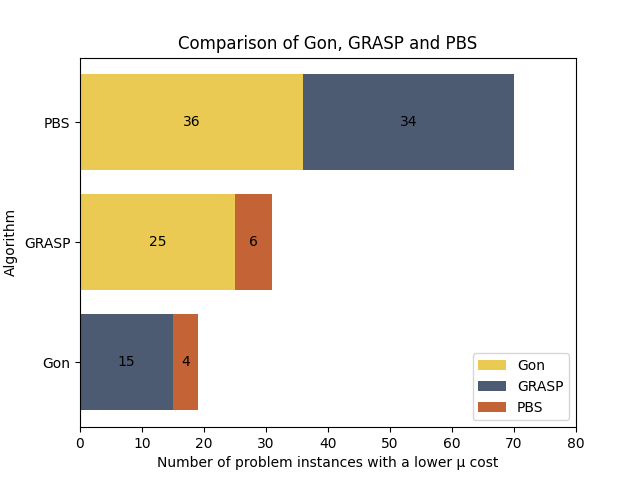
\includegraphics[width=0.65\textwidth]{images/compare_three_alg.png}
    \caption{Number of problem instances where an algorithm performed better than another}
    \label{fig:compare_three_alg}
\end{figure}
%TC:endignore

All three pairwise Quade tests returned a p-value below 0.05, we count the number of problem instances where one algorithm performed better than another in \cref{fig:compare_three_alg}. PBS achieved a lower cost than the \emph{Gon} algorithm in 36/40 and GRASP Plateau surfer in 34/40 ORLIB problems. Similarly the Plateau Surfer algorithm performed better than the \emph{Gon} in 25/40 problem instances. As the PBS algorithm is a memetic algorithm, there is variability in the results; we record the standard deviation in \cref{table:orlib_cost}. We calculate the cost $2\sigma$ above $\mu$ for PBS and the cost $2\sigma$ below $\mu$ for \emph{Gon}/Plateau Surfer, to account for 95.45\% of our observations under the empirical rule. Under this analysis, PBS achieves a lower cost than GRASP Plateau surfer for 34/40 and 31/40 for \emph{Gon} in ORLIB.

The average \%-gap above optimal cost was $\mu$ was 49.87\%, 47.83\% and 27.38\% for \emph{Gon}, Grasp Plateau Surfer and PBS respectively. While PBS performed significantly better than the other two algorithms, we could not reproduce results by \cite{pullan_memetic_2008} which showed the optimal optimal cost could be reached on all ORLIB problems. A possible reason could be the parameters for the strategy used to maintain population diversity which was not reported in their paper, we contacted the author via email for clarification but we did not receive a reply.
    
    \subsection{Colourful \texorpdfstring{$k$}{k}-center Gowalla data set}\label{section:colourful_k_center_gowalla}
    %TC:ignore
\begin{table}[H]
    \caption{Results on Gowalla instances}\label{table:gowalla_cost}
    \tiny
    \begin{tabularx}{\textwidth}{llXXXXlXXXXlXX}
    \firsthline
    \multicolumn{1}{c}{Instance}& \quad & \multicolumn{4}{c}{Pseudo $O(1)-approximation$}& \quad & \multicolumn{4}{c}{Colourful PBS} & \quad & \multicolumn{2}{c}{Statistics}\\
    \cline{1-1} \cline{3-6} \cline{8-11} \cline{13-14}\\
    name && min & $\mu$ & $\sigma$ & $\mu (time)$ && min & $\mu$ & $\sigma$ & $\mu (time)$ && \%-gap (cost) & \%-gap (time)\\
    \hline
    gow01 && 38.07 & 38.07 & 0.00 & 1.88 && 12.39 & 12.46 & 0.15 & 7.39 && -67.29 & 293.90\\
    gow02 && 2.27 & 2.27 & 0.00 & 1.80 && 1.11 & 1.13 & 0.00 & 6.50 && -50.18 & 261.76\\
    gow03 && 22.74 & 22.74 & 0.00 & 1.84 && 11.28 & 11.36 & 0.03 & 4.32 && -50.07 & 135.08\\
    gow04 && 2.70 & 2.70 & 0.00 & 0.85 && 1.35 & 1.35 & 0.00 & 3.27 && -50.00 & 282.54\\
    gow05 && 1.72 & 1.72 & 0.00 & 0.91 && 0.86 & 0.91 & 0.04 & 12.77 && -47.45 & 1301.59\\
    gow06 && 774.60 & 774.60 & 0.00 & 4.78 && 277.88 & 277.88 & 0.00 & 9.80 && -64.13 & 104.98\\
    gow07 && 52.34 & 52.34 & 0.00 & 2.11 && 26.46 & 26.50 & 0.23 & 8.65 && -49.38 & 310.12\\
    gow08 && 4.07 & 4.07 & 0.00 & 2.05 && 2.04 & 2.06 & 0.06 & 12.75 && -49.33 & 522.86\\
    gow09 && 4.19 & 4.19 & 0.00 & 1.97 && 2.10 & 2.17 & 0.04 & 24.10 && -48.13 & 1121.91\\
    gow10 && 1.32 & 1.32 & 0.00 & 1.96 && 0.75 & 0.80 & 0.02 & 34.81 && -39.48 & 1680.46\\
    gow11 && 1050.87 & 1050.87 & 0.00 & 9.23 && 495.18 & 509.63 & 2.96 & 18.94 && -51.50 & 105.04\\
    gow12 && 54.53 & 54.53 & 0.00 & 4.12 && 29.21 & 30.10 & 1.21 & 26.71 && -44.81 & 548.66\\
    gow13 && 9.80 & 9.80 & 0.00 & 3.69 && 4.94 & 5.61 & 0.39 & 29.28 && -42.78 & 693.81\\
    gow14 && 0.58 & 0.58 & 0.00 & 3.80 && 0.33 & 0.37 & 0.02 & 37.77 && -35.74 & 894.99\\
    gow15 && 2.59 & 2.59 & 0.00 & 3.84 && 1.39 & 1.75 & 0.19 & 37.20 && -32.46 & 869.05\\
    gow16 && 801.69 & 801.69 & 0.00 & 7.42 && 400.84 & 420.88 & 29.99 & 29.76 && -47.50 & 300.84\\
    gow17 && 379.08 & 379.08 & 0.00 & 12.93 && 188.74 & 189.19 & 1.34 & 42.57 && -50.09 & 229.22\\
    gow18 && 28.53 & 28.53 & 0.00 & 5.82 && 15.25 & 16.48 & 0.68 & 44.33 && -42.24 & 662.26\\
    gow19 && 6.49 & 6.49 & 0.00 & 5.72 && 3.28 & 3.67 & 0.14 & 52.57 && -43.43 & 818.83\\
    gow20 && 0.97 & 0.97 & 0.00 & 11.76 && 0.55 & 0.72 & 0.06 & 70.25 && -26.05 & 497.40\\
    gow21 && 898.02 & 898.02 & 0.00 & 21.39 && 308.76 & 351.59 & 22.84 & 51.36 && -60.85 & 140.15\\
    gow22 && 550.80 & 550.80 & 0.00 & 19.45 && 233.02 & 273.23 & 12.39 & 54.18 && -50.39 & 178.51\\
    gow23 && 16.65 & 16.65 & 0.00 & 8.75 && 8.54 & 9.07 & 0.89 & 55.69 && -45.56 & 536.39\\
    gow24 && 3.52 & 3.52 & 0.00 & 8.79 && 2.05 & 2.45 & 0.21 & 76.69 && -30.22 & 772.47\\
    gow25 && 1.31 & 1.31 & 0.00 & 17.73 && 0.77 & 0.92 & 0.08 & 74.68 && -29.60 & 321.26\\
    gow26 && 1038.79 & 1038.79 & 0.00 & 32.02 && 422.87 & 472.10 & 46.67 & 62.11 && -54.55 & 93.96\\
    gow27 && 341.32 & 341.32 & 0.00 & 27.08 && 170.29 & 205.67 & 29.69 & 61.28 && -39.74 & 126.32\\
    gow28 && 14.66 & 14.66 & 0.00 & 24.17 && 8.21 & 9.42 & 0.50 & 88.43 && -35.79 & 265.91\\
    gow29 && 3.46 & 3.46 & 0.00 & 24.29 && 1.96 & 2.24 & 0.23 & 104.95 && -35.27 & 332.02\\
    gow30 && 1.14 & 1.14 & 0.00 & 25.19 && 0.70 & 0.84 & 0.10 & 113.78 && -26.32 & 351.70\\
    gow31 && 1365.06 & 1365.06 & 0.00 & 44.23 && 523.64 & 658.87 & 56.73 & 76.46 && -51.73 & 72.88\\
    gow32 && 561.62 & 561.62 & 0.00 & 37.48 && 279.51 & 354.45 & 27.06 & 78.87 && -36.89 & 110.42\\
    gow33 && 11.52 & 11.52 & 0.00 & 34.83 && 6.70 & 8.02 & 1.31 & 108.16 && -30.40 & 210.58\\
    gow34 && 3.99 & 3.99 & 0.00 & 33.03 && 2.21 & 2.72 & 0.31 & 123.28 && -31.81 & 273.19\\
    gow35 && 1107.44 & 1107.44 & 0.00 & 25.69 && 554.25 & 708.06 & 97.53 & 75.15 && -36.06 & 192.51\\
    gow36 && 665.00 & 665.00 & 0.00 & 23.77 && 351.33 & 367.60 & 4.13 & 37.48 && -44.72 & 57.70\\
    gow37 && 645.74 & 645.74 & 0.00 & 24.45 && 334.58 & 396.61 & 26.57 & 75.02 && -38.58 & 206.78\\
    gow38 && 1161.61 & 1161.61 & 0.00 & 33.77 && 585.38 & 665.95 & 22.44 & 65.17 && -42.67 & 92.99\\
    gow39 && 618.42 & 618.42 & 0.00 & 60.81 && 277.00 & 357.25 & 39.18 & 93.95 && -42.23 & 54.50\\
    gow40 && 18.18 & 18.18 & 0.00 & 55.67 && 10.54 & 12.29 & 1.40 & 140.04 && -32.42 & 151.58\\
    \hline
    \multicolumn{1}{l}{Average} &&& 306.69 && 16.78 &&& 159.36 && 53.26 && -43.20 & 404.43\\
    \hline
    \multicolumn{5}{l}{Wilcoxon Signed Rank Test on mean costs:} & \multicolumn{9}{l}{p-value=\num{1.819e-12}}\\
        \lasthline
    \end{tabularx}
    \normalsize
\end{table}
%TC:endignore

\paragraph{Analysis of solution cost}~\\
Our result for the Wilcoxon test (\Cref{method:wilcoxon_test}) was \num{1.819e-12}, proving our observations to be statistically significant. From analysis using \Cref{method:counting_results}, colourful PBS produced lower costs than the \emph{Ban} algorithm for all 40 instances. The mean cost was 43.2\% lower on average.

To account for variance we conduct analysis using \Cref{method:counting_results_variance}. Using $\Delta =2$, which accounts for 95\% of the distribution, colorful \acrshort{pbs} outperforms \emph{Ban} for all 40 Gowalla problems. Furthermore if we take $\Delta =3$, which accounts for 99.7\% of the distribution, our algorithm still has lower costs for 39/40 problem instances.

\paragraph{Further analysis}~\\
We ran the brute force algorithm (\cref{alg:brute_force_colourful_k_center}) to obtain an optimal solution of a smaller 55 node problem instance (this took 5 hours and 16 minutes).

%TC:ignore
\begin{table}[H]
    \centering
    \tiny
    \caption{Performance on real world problem instance (gow41) with known optimal solution}
    \begin{tabular}{cccccccccccccccccc}
        \firsthline
        \multicolumn{4}{c}{Graph Details} & & \multicolumn{3}{c}{Constraints} & & \multicolumn{1}{c}{Optimal solution} & & \multicolumn{3}{c}{\emph{Ban} algorithm} & & \multicolumn{3}{c}{Colourful PBS}\\
        \cline{1-4} \cline{6-8} \cline{10-10} \cline{12-14} \cline{16-18}\\
         name &  n & blue & red & & k & min red & min blue & & optimal cost & & $\mu$ & $\sigma$ & \%-gap (opt) & & $\mu$ & $\sigma$ & \%-gap (opt)\\
         \hline
        gow41 & 55 & 15 & 40 & & 5 & 11 & 30 & & 577.26 & & 1089.92 & 0.00 & 88.81 & & 577.26 & 0.00 & 0.00\\
        \lasthline
    \end{tabular}
    \label{tab:brute_force_gowalla}
    \normalsize
\end{table}
%TC:endignore

Over 50 trials, colourful PBS converges to the optimal cost without fail whereas the \emph{Ban} algorithm achieves a cost 80\% above the optimal.

\begin{figure}[H]
    \centering
    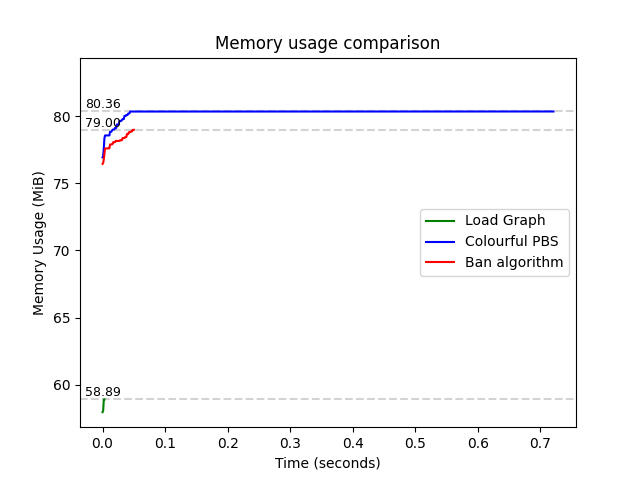
\includegraphics[width=0.7\textwidth]{images/memory_usage.png}
    \caption{Comparison of memory usage on gow41 problem instance\\ (dotted line indicates peak memory usage)}
    \label{fig:memory_usage}
\end{figure}

Analysing memory usage (\cref{fig:memory_usage}), colourful PBS uses 1.7\% more memory than \emph{Ban}, however this is insignificant compared to the memory required to store the graph which is around ~70\% of memory usage for both algorithms .

Overall for the real word 3D Gowalla data set Colourful PBS produces better results than the \emph{Ban} algorithm even after accounting for variance, however on average it incurs a five-fold increase in runtime.
    
    \subsection{Colourful \texorpdfstring{$k$}{k}-center Synthetic data set}\label{section:colourful_k_center_synthetic}
    %TC:ignore
\begin{table}[H]
    \caption{Results on Synthetic instances}\label{table:synthetic_cost}
    \tiny
    \begin{tabularx}{\textwidth}{XXlXXXXXlXXXXXlXX}
    \firsthline
    \multicolumn{2}{c}{Instance}& \hspace{0.25em} & \multicolumn{5}{c}{Pseudo $O(1)-approximation$}& \hspace{0.25em} & \multicolumn{5}{c}{Colourful PBS}& \hspace{0.25em} & \multicolumn{2}{c}{Statistics}\\
    \cline{1-2} \cline{4-8} \cline{10-14} \cline{16-17}\\
    name & opt && min & $\mu$ & $\sigma$ & \%-gap (opt) & $\mu (time)$ && min & $\mu$ & $\sigma$ & \%-gap (opt) & $\mu (time)$ && \%-gap (cost) & \%-gap (time)\\
    \hline
    syn01 & 133.50 && 267.00 & 267.00 & 0.00 & 100.00 & 1.09 && 133.50 & 133.50 & 0.00 & 0.00 & 0.94 && -50.00 & -14.18\\
    syn02 & 80.50 && 161.00 & 161.00 & 0.00 & 100.00 & 1.01 && 80.50 & 80.50 & 0.00 & 0.00 & 0.99 && -50.00 & -2.87\\
    syn03 & 40.50 && 81.00 & 81.00 & 0.00 & 100.00 & 0.99 && 40.50 & 40.50 & 0.00 & 0.00 & 1.23 && -50.00 & 23.46\\
    syn04 & 15.50 && 31.00 & 31.00 & 0.00 & 100.00 & 0.98 && 15.50 & 15.50 & 0.00 & 0.00 & 0.92 && -50.00 & -6.59\\
    syn05 & 80.50 && 1235.72 & 1235.72 & 0.00 & 1435.00 & 4.85 && 80.50 & 80.50 & 0.00 & 0.00 & 5.31 && -93.49 & 9.44\\
    syn06 & 40.50 && 81.00 & 81.00 & 0.00 & 100.00 & 2.16 && 40.50 & 40.50 & 0.00 & 0.00 & 2.08 && -50.00 & -3.70\\
    syn07 & 16.50 && 33.00 & 33.00 & 0.00 & 100.00 & 2.09 && 16.50 & 16.50 & 0.00 & 0.00 & 2.01 && -50.00 & -3.97\\
    syn08 & 8.50 && 17.00 & 17.00 & 0.00 & 100.00 & 2.25 && 8.50 & 9.01 & 2.02 & 6.00 & 9.78 && -47.00 & 333.99\\
    syn09 & 80.50 && 626.95 & 626.95 & 0.00 & 679.00 & 9.50 && 80.50 & 80.50 & 0.00 & 0.00 & 10.63 && -87.16 & 11.98\\
    syn10 & 27.50 && 339.95 & 339.95 & 0.00 & 1136.00 & 8.61 && 27.50 & 27.80 & 0.41 & 1.00 & 20.66 && -91.82 & 139.96\\
    syn11 & 12.50 && 25.00 & 25.00 & 0.00 & 100.00 & 3.84 && 12.50 & 12.50 & 0.00 & 0.00 & 3.78 && -50.00 & -1.60\\
    syn12 & 5.50 && 11.00 & 11.00 & 0.00 & 100.00 & 4.40 && 5.50 & 5.50 & 0.00 & 0.00 & 3.99 && -50.00 & -9.31\\
    syn13 & 80.50 && 873.77 & 873.77 & 0.00 & 985.00 & 15.51 && 80.50 & 80.50 & 0.00 & 0.00 & 20.12 && -90.79 & 29.78\\
    syn14 & 16.50 && 169.22 & 169.22 & 0.00 & 926.00 & 12.98 && 16.50 & 17.05 & 1.84 & 3.00 & 36.08 && -89.92 & 177.96\\
    syn15 & 12.50 && 25.00 & 25.00 & 0.00 & 100.00 & 6.45 && 12.50 & 12.50 & 0.00 & 0.00 & 8.10 && -50.00 & 25.51\\
    syn16 & 4.50 && 9.00 & 9.00 & 0.00 & 100.00 & 6.46 && 9.00 & 9.00 & 0.00 & 100.00 & 6.27 && -0.00 & -2.93\\
    syn17 & 80.50 && 1319.61 & 1319.61 & 0.00 & 1539.00 & 25.63 && 80.50 & 80.50 & 0.00 & 0.00 & 29.97 && -93.90 & 16.93\\
    syn18 & 16.50 && 223.42 & 223.42 & 0.00 & 1254.00 & 20.90 && 16.50 & 26.23 & 33.01 & 59.00 & 47.35 && -88.26 & 126.53\\
    syn19 & 12.50 && 142.10 & 142.10 & 0.00 & 1037.00 & 21.44 && 12.50 & 12.50 & 0.00 & 0.00 & 25.29 && -91.20 & 17.93\\
    syn20 & 3.50 && 7.00 & 7.00 & 0.00 & 100.00 & 10.21 && 3.50 & 4.90 & 1.71 & 40.00 & 52.17 && -30.00 & 411.22\\
    syn21 & 80.50 && 655.34 & 655.34 & 0.00 & 714.00 & 36.65 && 80.50 & 80.50 & 0.00 & 0.00 & 45.39 && -87.72 & 23.84\\
    syn22 & 16.50 && 33.00 & 33.00 & 0.00 & 100.00 & 15.13 && 16.50 & 16.50 & 0.00 & 0.00 & 13.83 && -50.00 & -8.56\\
    syn23 & 9.50 && 19.00 & 19.00 & 0.00 & 100.00 & 14.51 && 9.50 & 9.50 & 0.00 & 0.00 & 13.10 && -50.00 & -9.75\\
    syn24 & 2.50 && 5.00 & 5.00 & 0.00 & 100.00 & 14.60 && 2.50 & 4.05 & 1.21 & 62.00 & 45.36 && -19.00 & 210.76\\
    syn25 & 40.50 && 81.00 & 81.00 & 0.00 & 100.00 & 20.66 && 40.50 & 46.45 & 10.94 & 15.00 & 54.37 && -42.65 & 163.15\\
    syn26 & 11.50 && 154.75 & 154.75 & 0.00 & 1246.00 & 38.49 && 83.38 & 102.85 & 20.73 & 794.00 & 88.30 && -33.54 & 129.43\\
    syn27 & 8.50 && 127.50 & 127.50 & 0.00 & 1400.00 & 39.75 && 64.92 & 85.67 & 16.36 & 908.00 & 94.16 && -32.81 & 136.90\\
    syn28 & 2.50 && 5.00 & 5.00 & 0.00 & 100.00 & 19.71 && 2.50 & 4.00 & 1.22 & 60.00 & 65.47 && -20.00 & 232.13\\
    syn29 & 40.50 && 407.80 & 407.80 & 0.00 & 907.00 & 55.13 && 40.50 & 100.25 & 90.45 & 148.00 & 72.68 && -75.42 & 31.83\\
    syn30 & 11.50 && 93.76 & 93.76 & 0.00 & 715.00 & 49.59 && 11.50 & 35.84 & 22.25 & 212.00 & 73.27 && -61.78 & 47.75\\
    syn31 & 7.50 && 80.59 & 80.59 & 0.00 & 975.00 & 50.47 && 48.50 & 56.66 & 5.78 & 655.00 & 67.70 && -29.69 & 34.13\\
    syn32 & 2.50 && 5.00 & 5.00 & 0.00 & 100.00 & 24.62 && 2.50 & 4.20 & 1.17 & 68.00 & 73.95 && -16.00 & 200.37\\
    syn33 & 27.50 && 322.65 & 322.65 & 0.00 & 1073.00 & 67.32 && 27.50 & 27.50 & 0.00 & 0.00 & 83.11 && -91.48 & 23.45\\
    syn34 & 10.50 && 157.83 & 157.83 & 0.00 & 1403.00 & 69.09 && 69.78 & 112.00 & 26.39 & 967.00 & 88.80 && -29.04 & 28.52\\
    syn35 & 7.50 && 61.64 & 61.64 & 0.00 & 722.00 & 69.08 && 7.50 & 28.75 & 9.27 & 283.00 & 70.49 && -53.36 & 2.04\\
    syn36 & 2.50 && 5.00 & 5.00 & 0.00 & 100.00 & 34.51 && 2.50 & 4.30 & 1.12 & 72.00 & 59.47 && -14.00 & 72.33\\
    syn37 & 80.50 && 161.00 & 161.00 & 0.00 & 100.00 & 1.02 && 80.50 & 80.50 & 0.00 & 0.00 & 0.82 && -50.00 & -19.99\\
    syn38 & 40.50 && 81.00 & 81.00 & 0.00 & 100.00 & 4.52 && 40.50 & 40.50 & 0.00 & 0.00 & 3.88 && -50.00 & -14.05\\
    syn39 & 16.50 && 33.00 & 33.00 & 0.00 & 100.00 & 15.05 && 16.50 & 16.50 & 0.00 & 0.00 & 13.54 && -50.00 & -9.99\\
    syn40 & 13.50 && 27.00 & 27.00 & 0.00 & 100.00 & 35.42 && 13.50 & 13.50 & 0.00 & 0.00 & 30.07 && -50.00 & -15.11\\
    \hline
    \multicolumn{2}{l}{Average} &&&&& 511.15 & 20.92 &&&&& 111.32 & 33.64 && -54.00 & 63.47\\
    \hline
    \multicolumn{5}{l}{Wilcoxon Signed Rank Test on mean costs:} & \multicolumn{9}{l}{p-value=\num{1.819e-12}}\\
        \lasthline
    \end{tabularx}
    \normalsize
\end{table}
%TC:endignore

\paragraph{Analysis of solution cost}~\\
We report statistically significant results for the synthetic data set, with a p-value of \num{1.819e-12} for the Wilcoxon test. Colourful PBS achieves a lower cost than the O(1)-approximation for 39/40 Gowalla instances. The average gap between the optimal solution and the $O(1)$-approximation was 511.15\%, our algorithm produced solutions significantly closer to the optimal, with an of average 111.32\% above the optimal cost. The average \%-gap for the optimal cost for Colourful PBS was skewed by five instances which were over 600\% above the optimal cost, namely syn26, syn27, syn31, syn34 and syn35. In terms of achieving the optimal cost, Colourful PBS return the optimal solution for 22/40 synthetic problems (with 100\% accuracy over 50 repeats), while the $O(1)$-approximation achieved the optimal cost for none of the problems.

If we conduct the same analysis to account for memetic algorithm variablility in \cref{section:colourful_k_center_gowalla}, our algorithm outperforms the $O(1)$-approximation for 34/40 instances for $2\sigma$ above $\mu$ and 31/40 for $3\sigma$ above $\mu$. Clearly even accounting for variability, our algorithm produces solutions with lower costs for over 75\% of synthetic problem instances.

\section{Evaluation}\label{section:evaluation}
    \subsection{Colourful PBS}
    Through our statistical analysis in \cref{section:colourful_k_center_gowalla} and \cref{section:colourful_k_center_synthetic} our algorithm proved to be conclusively better than the \emph{Ban} algorithm. Across 4000 trials over 80 problem instances (Gowalla and Synthetic), Colourful PBS produces solutions with a 48.6\% lower cost than the algorithm by \citeauthor{bandyapadhyay_constant_2019}, at the expense of a 3.3-fold increase in runtime. This increase in runtime is partly due to running the \emph{Ban} algorithm as a subroutine to seed the population. Given more time, we would explore alternative population generation methods to allow for quicker convergence.

Furthermore if we were to extend the scope of our project, we would have also liked to implement two recent algorithms for the Colourful $k$-center by \textcite{jia_fair_2020} and \textcite{anegg_technique_2020}. Gaining empirical results for these theoretical algorithms would allow us to make stronger conclusions on the performance of Colourful PBS.  
    
    \subsection{The web tool}
    The home page of our website is shown in \cref{fig:home_page}, the user can access our two main tools through the buttons "solve a graph" and "visualise steps to a solution". In addition we added a section that extended our original scope of our tool, "what is the colourful $k$-center" to introduce the colourful $k$-center problem to users through an example. Although this feature was not part of our original set of requirements, we introduced a step by step example to explain the relationship between the $k$-center and colourful $k$-center, based on the analogies described in \cref{section:k_center}, \cref{section:robust_k_center} and \cref{section:colourful_k_center}. We felt that this served as a gentle introduction to $k$-center problems.

%TC:ignore
\begin{figure}[H]
    \centering
    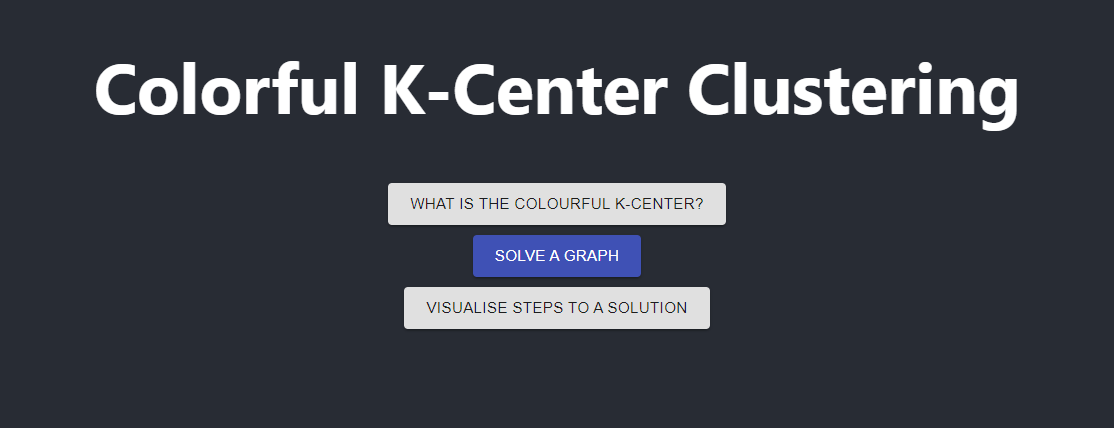
\includegraphics[width=0.75\textwidth]{images/home_page.png}
    \caption{Website home page}
    \label{fig:home_page}
\end{figure}
%TC:endignore

\paragraph{Solution Visualisation}~\\
We created a online tool which implements and visualises all five algorithms described in this paper. Implementing these algorithms served as a good introduction to our understanding of a variety of programming paradigms, including approximation, randomised and memetic algorithms. In addition to fulfilling the primary visualisation requirement, we add quality of life features such as tooltips and an interactive legend (\cref{fig:solve_app}).

%TC:ignore
\begin{figure}[H]
    \centering
    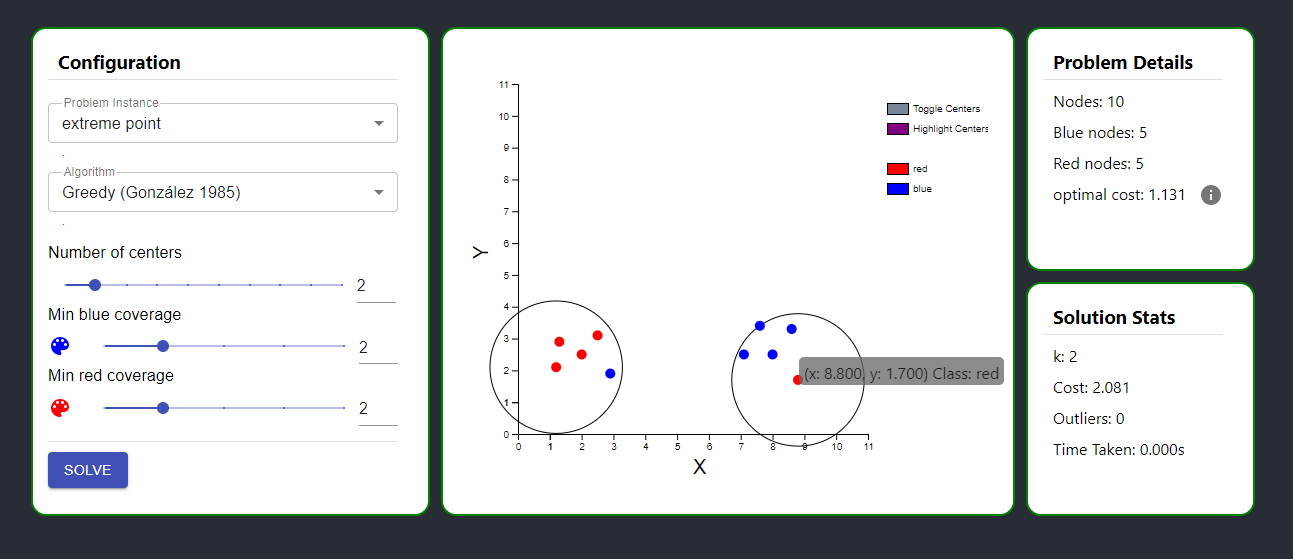
\includegraphics[width=0.85\textwidth]{images/solve_app.png}
    \caption{"solve a graph" web page}
    \label{fig:solve_app}
\end{figure}
%TC:endignore

While tool has the ability to adjust all parameters for the problem instance, there lacks configuration for each individual algorithm. For example, our algorithm implementations have the ability to halt as soon as a target cost or a timeout is reached; this functionality is accessible through the command line but not through the web tool.

\paragraph{Interactive Algorithm Visualisation}~\\
We also provide a tool to show how all five algorithms work step by step. While simpler algorithms such as \emph{Gon} would be understandable to a user without being familiar with the algorithm beforehand, algorithms such as PBS would require prior understanding. If we were reattempt this task, we would add supporting visualisations to show which part of the pseudocode was currently being executed. 

In terms of the genetic algorithm visualisation aspect (see \cref{section:stepped_visualisation}), we believe our design which allows viewing of both the whole population and specific individuals aided our understanding of genetic algorithms. One minor improvement we would make is to highlight specific individuals which were modified between local searches and generations.

A more ambitious extension of our tool would be to add animations to each step to highlight either swaps between centers or opening of new centers. From an educational viewpoint, the effectiveness of this tool remains to be proven. However as far as aiding our own understanding of the algorithms, we believe it has achieved its role.

\paragraph{Accessibility}~\\
Our tool can be accessed at \url{https://colourful-k-center.herokuapp.com}. Considering our project covers algorithms that use LP solvers, this tool provides a way to visualise the O(1)-approximation algorithm without needing to install a solver such as GLPK. Should the user want to run their own instance either locally or on the web, the application is packaged into a Docker image, with build and deploy only requiring two commands (\cref{fig:docker_setup}).

%TC:ignore
\begin{figure}[H]
    \centering
    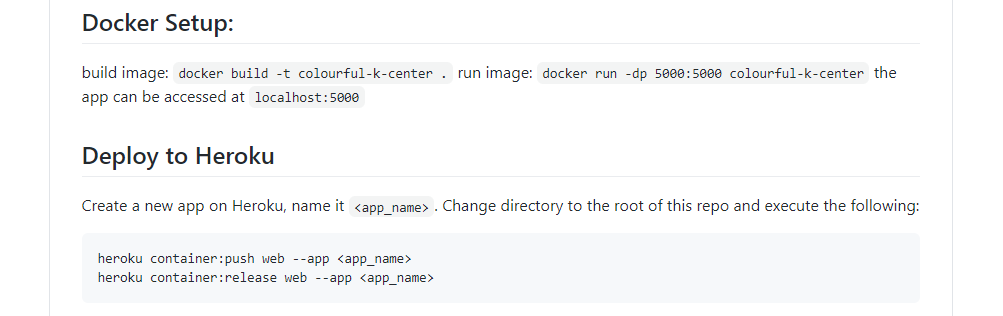
\includegraphics[width=0.85\textwidth]{images/docker_setup.png}
    \caption{Instructions for setting up our web tool using Docker}
    \label{fig:docker_setup}
\end{figure}
%TC:endignore

If a researcher wishes to utilise/extend our code, they would need to install the Python pip dependencies, an LP solver and R (for statistical analysis). Although the latter two dependencies are slightly more involved to install, there are detailed installation guides for both GLPK and R online.
    
    \subsection{Software Engineering}
    To ensure our code works correctly we wrote unit tests in pytest for the server code. Our tests cover functionality of each algorithm on small instances ($n\leq 25$) and the subroutines they use such as the PBS local search. In total, we have 186 tests covering 97.05\% lines of code. 

We chose to not write unit tests for the front end as they are tedious to maintain which would slow down our development. Instead we wrote end to end tests, which covers the all website pages using Cypress. The end to end tests go through each page, takes a screenshot and then compares it to a saved snapshot. If they are not the same, we manually inspect it to ensure the visual change is as expected. We believe the screenshot regression tests ensured our core functionality did not regress between major changes to our website. If we were to target our application for a production environment, we would write a suite of unit tests to cover edge cases for the \acrshort{ui}.

We also used tools monitor the health of our app during development. We used Github actions to automatically run the tests and produce a CodeCov report for every pull request, with quality checks failing if our code coverage was below the coverage of the main branch. Continuous integration was important for our workflow as it ensured any code going into the main branch as both passing tests and sufficiently tested.
    
    \subsection{Reflection}
    We started this project with knowledge in Python, \acrshort{js} and React. This project has allowed us to learn new languages, through the use of TypeScript for our web tool and R for our statistical analysis. We have also gained knowledge in new libraries such as Pyomo (Linear programming), D3.js (graphing) and Flask (web framework). We have also been exposed to modern technologies, from using Cypress for our regression tests and Docker for deploying our application.

From an academic viewpoint, we started the project with zero knowledge in linear programming, approximation algorithms and genetic algorithms. We believe we have built strong foundations in those topics through conducting our study. In particular we believe our new knowledge about linear programs will allow us to access a wider range of academic papers and optimisation problems in general.
    
\section{Discussion}\label{section:discussion}
Overall this project achieved its two aims of proposing a new algorithm for the colourful $k$-center problem and creating an algorithm visualisation tool.

\paragraph{Educational Value}~\\
We believe our web tool serves as a good introduction to $k$-center problems, shows clear visualisation of solutions and offers coherent step by step visualisations for basic algorithms such as the \emph{Gon} algorithm. While interactive visualisations are less concise with more complex algorithms such as GRASP and PBS, we believe with further work it has the potential to be an valuable educational aid.

\paragraph{Future Work}~\\
Our code has been documented and tested, so that another group can easily pick up and expand on our work. Colourful PBS relies on population seeding to produce good solutions, while we use the pseudo 2-approximation as a subroutine to seed our population, it takes a considerable amount of time; further work could investigate more efficient subroutines to produce seed solutions which are good starting points without having to run an expensive linear program.

Another avenue to be explored is research into new genetic operators. While we used the PBS genetic operators for colourful PBS, it is plausible there are genetic operators that could be tailored to the colourful $k$-center.

\paragraph{Open Questions}~\\
One open question would be to whether the performance of our algorithm extends to a large number of demographic groups. In our study we have looked at \gls{approx_algs} and \gls{metaheuristic} approaches to the colourful $k$-center. While we have shown a na\"ive brute force algorithm, another open question would be to find an efficient \gls{exact_algs} algorithm.


\section{Conclusion}\label{section:conclusion}
This project studies the $k$-center and colourful $k$-center problems; the former is a classical NP-hard problem and the latter is an extension to the $k$-center relevant to fair machine learning. We evaluated algorithms from approximation, genetic and randomised algorithm paradigms for solving the $k$-center, then used these findings to propose a new \gls{memetic_algs} algorithm for the colourful $k$-center, named colourful PBS. We showed colourful PBS produced solutions with lower costs than the existing pseudo 2-approximation algorithm. However we note that the increase in performance is at the expense of run time. In addition, we create a web tool to visualise solutions with the aim to educate a user about $k$-center problems and their related algorithms. 

\subsection{Discussion}
Overall this project achieved its two aims of proposing a new algorithm for the colourful $k$-center problem and creating an algorithm visualisation tool.

\paragraph{Educational Value}~\\
We believe our web tool serves as a good introduction to $k$-center problems, shows clear visualisation of solutions and offers coherent step by step visualisations for basic algorithms such as the \emph{Gon} algorithm. While interactive visualisations are less concise with more complex algorithms such as GRASP and PBS, we believe with further work it has the potential to be an valuable educational aid.

\paragraph{Future Work}~\\
Our code has been documented and tested, so that another group can easily pick up and expand on our work. Colourful PBS relies on population seeding to produce good solutions, while we use the pseudo 2-approximation as a subroutine to seed our population, it takes a considerable amount of time; further work could investigate more efficient subroutines to produce seed solutions which are good starting points without having to run an expensive linear program.

Another avenue to be explored is research into new genetic operators. While we used the PBS genetic operators for colourful PBS, it is plausible there are genetic operators that could be tailored to the colourful $k$-center.

\paragraph{Open Questions}~\\
One open question would be to whether the performance of our algorithm extends to a large number of demographic groups. In our study we have looked at \gls{approx_algs} and \gls{metaheuristic} approaches to the colourful $k$-center. While we have shown a na\"ive brute force algorithm, another open question would be to find an efficient \gls{exact_algs} algorithm.

    
\newpage
%TC:ignore
\section{References}
\sloppy{\printbibliography[heading=none]}

\appendix
\section{Brute Force Algorithms}
    \subsection{k-center}
        \label{brute-force-k-center}
        %TC:ignore
\begin{algorithm}[H] 
\caption{Find cost of K-Center Solution}
\label{alg:brute_force_k_center}
\begin{algorithmic}[1]
\Statex
\Function{Find\_K\_Center\_Cost}{$S$}
    \State {$max\_cost$ $\gets$ {$0$}}
    \For{$p \gets 1$ to $N$}
        \State {$min\_cost$ $\gets$ {$max(d_{ij})$}}
        \For{$s \gets 1$ to $|S|$}
            \State {$cost$ $\gets$ {$dist(P_i, P_s)$}}
            \If{$cost < min\_cost$}
                \State {$min\_cost$ $\gets$ {$cost$}}
            \EndIf
        \EndFor
        \If{$min\_cost$ $>$ {$max\_cost$}}
            \State {$max\_cost$ $\gets$ {$min\_cost$}}
        \EndIf
    \EndFor
    \State \Return {$max\_cost$}
\EndFunction
\end{algorithmic}
\end{algorithm}

\begin{algorithm}[H] 
\caption{Brute force Colourful K-Center solution}
\label{alg:k_center_cost}
\begin{algorithmic}[1]
\Statex
\Function{Candidate\_Combination}{$L, k, Partial$}
    \If{$k < 1$}
        \State {$cost$ $\gets$ {$Find\_K\_Center\_Cost(Partial)$}}
        \If{$cost < min\_cost$}
            \State {$min\_cost$ $\gets$ {$p$}}
            \State {$best\_solution$ $\gets$ {$Partial$}}
        \EndIf
    \EndIf
    \For{$i \gets 1$ to $|L|$}
        \State {$Candidate\_Combination(L_{i+1,|L|}, k-1, Partial + L_i)$}
    \EndFor
\EndFunction
\Statex
\Procedure{Brute\_Force\_K\_Center}{}
    \State {$min\_cost$ $\gets$ {$max(d_{ij})$}}
    \State {$best\_solution$ $\gets$ {$\emptyset$}}
    \State {$Candidate\_Combination(P, k,\emptyset)$}
    
\EndProcedure
\end{algorithmic}
\end{algorithm}
%TC:endignore
    \subsection{colourful k-center}
        \label{brute-force-colourful-k-center}
        %TC:ignore
\begin{algorithm}[H] 
\caption{Verify if centers and cost meet the minimum cover constraints}
\label{alg:brute_force_colourful_k_center}
\begin{algorithmic}[1]
\Statex
\Function{Verify\_Colourful\_Solution}{$S, p$}
    \State {$b'$ $\gets$ {$0$}}
    \State {$r'$ $\gets$ {$0$}}
    \For{$p \gets 1$ to $N$}
        \State {$point\_covered$ $\gets$ {$False$}}
        \For{$s \gets 1$ to $|S|$}                    
            \If{$dist(P_i, P_s) \leq p$}
                \State {$point_covered$ $\gets$ {$True$}}
            \EndIf
        \EndFor
        \If{$point\_covered$ $=$ {$True$}}
            \If{$P_i \in B$}
                \State {$b'$ $\gets$ {$b' + 1$}}
            \ElsIf{$P_i \in R$}
                \State {$r'$ $\gets$ {$r' + 1$}}
            \EndIf
        \EndIf
    \EndFor
    \State \Return {$r' \geq r$ \&\& $b' \geq b$}
\EndFunction
\end{algorithmic}
\end{algorithm}

\begin{algorithm}[H] 
\caption{Brute force Colourful K-Center solution}
\label{alg:colourful_k_center_valid}
\begin{algorithmic}[1]
\Statex
\Function{Candidate\_Combination}{$L, k, p, Partial$}
    \If{$k < 1$}
        \State {$valid$ $\gets$ {$Verify\_Colourful\_Solution(Partial, p)$}}
        \If{$valid$ \&\& $p < min\_cost$}
            \State {$min\_cost$ $\gets$ {$p$}}
            \State {$best\_solution$ $\gets$ {$Partial$}}
        \EndIf
    \EndIf
    \For{$i \gets 1$ to $|L|$}
        \State {$Candidate\_Combination(L_{i+1,|L|}, k-1, p, Partial + L_i)$}
    \EndFor
\EndFunction
\Statex
\Procedure{Brute\_Force\_Colourful\_K\_Center}{}
    \State {$min\_cost$ $\gets$ {$max(d_{ij})$}}
    \State {$best\_solution$ $\gets$ {$\emptyset$}}
    \For{$i \gets 1$ to $N$}
        \For{$j \gets 1$ to $N$}
            \State {$Candidate\_Combination(P, k, dist(i, j),\emptyset)$}
        \EndFor
    \EndFor
    
\EndProcedure
\end{algorithmic}
\end{algorithm}
%TC:endignore
        %TC:ignore
\begin{algorithm}[H] 
\caption{Generate Random Colourful $k$-center problem instance}
\label{alg:generate_colourful}
\begin{algorithmic}[1]
\Require $b/r$: num blue/red points, $o$: num outliers, $k$: num centers, $\rho$: optimal cost
\Ensure 
\Procedure{generate\textunderscore colourful}{$b, r,o,k,\rho$}
    \State{$Q\gets$ create randomised queue of $elements\in \{blue, red\}$ with $b$ $blue$ elements and $r$ $red$ elements}
    \State{$V\gets\emptyset$}\Comment{Each time a node is added to $V$, a colour is assigned to the node by popping from $Q$\hphantom{......................................}}
    \State{$C\gets$ generate $k$ nodes at least $\rho$ pairwise distance apart}
    \State{}
    \State{$S\gets$ generate 2 supporting points per node $c\in C$ that connect to make a line passing through $c$ with length $2\rho$}
    \State{$i\gets (b + r) - (o + |C| + |S|)$}
    \State{$I\gets$ generate $i$ nodes uniformly around nodes $c\in C$ at most $\rho$ distance away from $c$}
    \State{$O\gets$ generate $o$ nodes uniformly anywhere more than $\rho distance from any c\in C$}
    \State{}
    \State{$V\gets V\cup C\cup S\cup I\cup O$}
    \State\Return{$V$}
\EndProcedure
\end{algorithmic}
\end{algorithm}
%TC:endignore
\section{Determining parameters for GRASP}\label{appendix:grasp_param}
    We performed grid search for the parameters $\alpha$ and $\beta$ for values between 0 and 1. The data set we used was TSPLIB, originally a travelling salesman data set that has been used for $k$-center, which has known optimal $k$-center costs for some instances (\cite{pullan_memetic_2008}). For each parameter pair, we perform 5 trails with 5 iterations, therefore the local search is performed 25 times. We then calculate the mean percentage above the optimal cost, and plot it in a heatmap in \cref{fig:grid_search_heatmap}.

\begin{figure}[H]
    \centering
    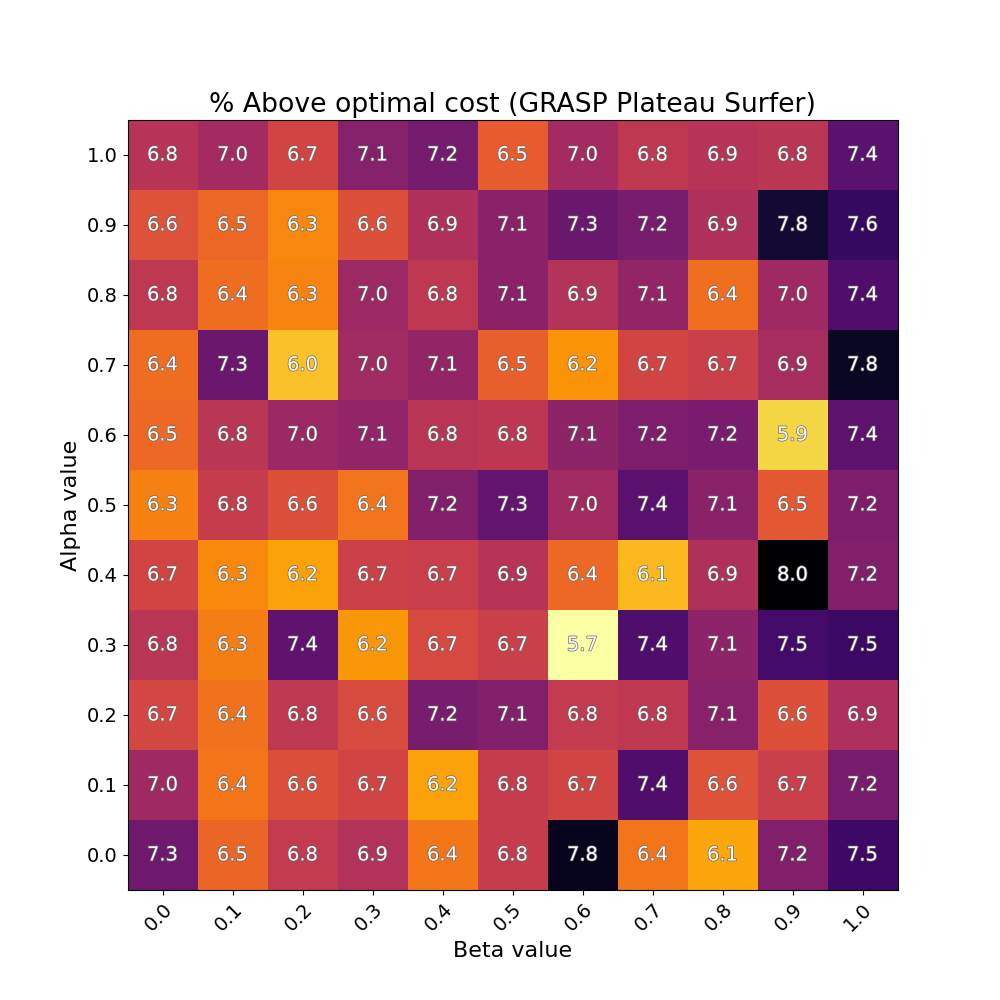
\includegraphics[height=13cm]{images/grasp_heatmap.png}
    \caption{Grasp Plateau Surfer grid search}
    \label{fig:grid_search_heatmap}
\end{figure}

The average percentage above optimal cost for each quadrant is shown in \cref{fig:grid_search_quadrant}.

\begin{figure}[H]
    \centering
    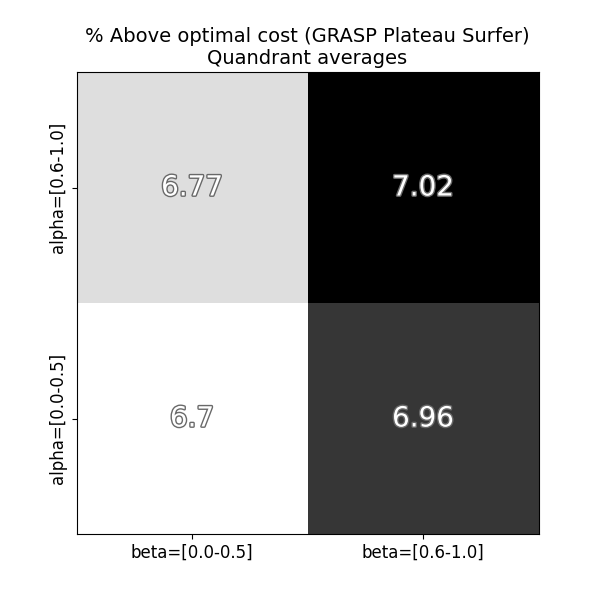
\includegraphics[height=7cm]{images/quadrant_averages_grasp.png}
    \caption{Grasp Plateau Surfer grid search (quadrant averages)}
    \label{fig:grid_search_quadrant}
\end{figure}
    
\section{Comparing genetic architectures}\label{appendix:genetic_architectures}
    When designing colourful PBS, we noted PBS uses an non-standard genetic selection method where the population is updated as soon as a better solution is found (this is somewhat similar to elitism selection). The impact is the diversity of the population may be reduced, therefore we also tested roulette and tournament selection. We generated a small training set of 10 problems using the procedure described in \cref{alg:generate_colourful} and conducted 50 trials setting a time limit of $0.15n+0.5k$ seconds (our full methodology is described in \cref{section:methodology}). Our results are reported in \cref{table:compare_genetic}.

%TC:ignore
\begin{table}[H]
    \caption{Results on training set for different genetic selection operators}\label{table:compare_genetic}
    \footnotesize
    \begin{tabularx}{\textwidth}{lllllllXXXlXXXlXXX}
    \firsthline
    \multicolumn{6}{c}{Instance} & \quad & \multicolumn{3}{c}{Original PBS Selection} & \quad & \multicolumn{3}{c}{Roulette Selection} & \quad & \multicolumn{3}{c}{Tournament Selection} \\
    \cline{1-6} \cline{8-10} \cline{12-14} \cline{16-18}
    Name & n & k & b & r & opt && $min$ &$\mu$ & $\sigma$ && $min$ &$\mu$ & $\sigma$ && $min$ &$\mu$ & $\sigma$\\
    \hline
    train01 & 100 & 5 & 40 & 40 & 15.50 && 15.50 & 15.50 & 0.00 && 15.50 & 15.50 & 0.00 && 15.50 & 15.50 & 0.00\\
    train02 & 100 & 10 & 40 & 40 & 12.50 && 12.50 & 12.50 & 0.00 && 12.50 & 12.53 & 0.18 && 12.50 & 12.58 & 0.31\\
    train03 & 100 & 20 & 40 & 40 & 6.50 && 6.50 & 6.52 & 0.07 && 6.50 & 7.15 & 0.49 && 6.50 & 6.99 & 0.44\\
    train04 & 200 & 5 & 90 & 90 & 4.50 && 4.50 & 4.50 & 0.00 && 4.50 & 4.50 & 0.00 && 4.50 & 4.50 & 0.00\\
    train05 & 200 & 10 & 90 & 90 & 11.50 && 11.50 & 11.50 & 0.00 && 11.50 & 11.50 & 0.00 && 11.50 & 11.50 & 0.00\\
    train06 & 200 & 20 & 90 & 90 & 22.50 && 22.50 & 28.09 & 3.50 && 22.50 & 29.75 & 2.06 && 22.50 & 29.18 & 2.77\\
    train07 & 300 & 20 & 130 & 130 & 23.50 && 23.50 & 23.50 & 0.00 && 23.50 & 23.90 & 1.19 && 23.50 & 23.82 & 1.08\\
    train08 & 300 & 40 & 130 & 130 & 43.50 && 582.93 & 684.75 & 138.11 && 582.93 & 900.37 & 102.79 && 582.93 & 839.51 & 152.00\\
    train09 & 400 & 20 & 170 & 170 & 33.50 && 33.50 & 367.41 & 668.32 && 33.50 & 704.83 & 823.10 && 33.50 & 897.84 & 831.45\\
    train10 & 400 & 40 & 170 & 170 & 53.50 && 623.81 & 1231.79 & 156.93 && 623.81 & 1312.21 & 155.16 && 697.47 & 1267.48 & 145.36\\
    \hline
    \multicolumn{6}{l}{Average \% cost above opt} && \multicolumn{3}{c}{469.84\%} && \multicolumn{3}{c}{637.06\%} && \multicolumn{3}{c}{671.84\%}\\
    \hline
    \multicolumn{6}{l}{Omnibus Quade test: p-value = 0.0204} & \multicolumn{11}{c}{}\\
    \lasthline
    \end{tabularx}
    \normalsize
\end{table}

%TC:endignore


All three methods achieved near optimal costs for train 1-7, however they all performed poorly on the larger instances train 8-10. In all intances the original PBS selection method performed equal to or better than the other two. To determine whether these results are statistically significant we performed a Quade test on the mean cost for each instance and algorithm; a statistically significant result would have a p-value below $\alpha =0.05$. Our resulting p-value is 0.02, showing the three methods are statistically significant. To determine which algorithms are statistically significant from eachother, we perform a post-hoc pairwise Quade test shown in \cref{table:compare_genetic_quade}.

%TC:ignore
\begin{table}[H]
    \centering
    \caption{P-values from Post-hoc pairwise Quade test (on results from \cref{table:compare_genetic})}\label{table:compare_genetic_quade}
    \begin{tabularx}{0.75\textwidth}{|X|XX|}
        \hline
        \textbf{Algorithm} & Original PBS & Roulette Selection\\
        \hline
        Roulette Selection & 0.0225 & N/A\\
        Tournament Selection & 0.0795 & 0.4373\\
        \lasthline
    \end{tabularx}
\end{table}
%TC:endignore

The original PBS selection method is statistically significant and better than roulette selection, since $0.0225<0.05$ and it produced better results in 7/10 instances. Original PBS is also statistically significant from tournament selection although to a lesser degree since it falls under the 90\% confidence interval as $0.0795<0.1$, on average it produced results with lower cost for 7/10 instances. The differences between tournament and roulette selection are insignificant as $0.4373>0.1$. We concluded the original PBS selection method was the best, as we obtained statistically significant samples and it outperformed roulette and tournament selection for the majority of the training set.
    
\section{Seeding the genetic population}\label{appendix:seed_population}
    In preliminary tests for colourful PBS, we found some instances failed to converge due to the search being stuck in local minima from their initial starting points being on outliers or having multiple centers in close proximity of eachother. The centers produced by the pseudo apporximation (\cref{section:constant_colourful_k_center}) produced centers which cover many points and therefore away from outliers, we use this algorithm as a subroutine to seed the first individual the population of our genetic algorithm, the remainder of the population is generated as before. The result of this is significantly better performance on our training set shown in \cref{table:improved_colourful_pbs}.

%TC:ignore
\begin{table}[H]
    \caption{Results before and after population seeding}\label{table:improved_colourful_pbs}
    \footnotesize
    \begin{tabularx}{\textwidth}{lllllllXXXlXXX}
    \firsthline
    \multicolumn{6}{c}{Instance} & \quad & \multicolumn{3}{c}{Colourful PBS} & \quad & \multicolumn{3}{c}{Colourful PBS + Population Seeding}\\
    \cline{1-6} \cline{8-10} \cline{12-14}
    Name & n & k & b & r & opt && $min$ &$\mu$ & $\sigma$ && $min$ &$\mu$ & $\sigma$\\
    \hline
    train01 & 100 & 5 & 40 & 40 & 15.50 && 15.50 & 15.50 & 0.00 && 15.50 & 15.50 & 0.00\\
    train02 & 100 & 10 & 40 & 40 & 12.50 && 12.50 & 12.50 & 0.00 && 12.50 & 12.50 & 0.00\\
    train03 & 100 & 20 & 40 & 40 & 6.50 && 6.50 & 6.52 & 0.07 && 6.50 & 6.53 & 0.10\\
    train04 & 200 & 10 & 90 & 90 & 11.50 && 11.50 & 11.50 & 0.00 && 11.50 & 11.50 & 0.00\\
    train05 & 200 & 5 & 90 & 90 & 4.50 && 4.50 & 4.50 & 0.00 && 4.50 & 4.50 & 0.00\\
    train06 & 200 & 20 & 90 & 90 & 22.50 && 22.50 & 28.09 & 3.50 && 22.50 & 28.01 & 3.61\\
    train07 & 300 & 20 & 130 & 130 & 23.50 && 23.50 & 23.50 & 0.00 && 23.50 & 23.50 & 0.00\\
    train08 & 300 & 40 & 130 & 130 & 43.50 && 582.93 & 684.75 & 138.11 && 43.50 & 43.50 & 0.00\\
    train09 & 400 & 20 & 170 & 170 & 33.50 && 33.50 & 367.41 & 668.32 && 33.50 & 428.20 & 702.49\\
    train10 & 400 & 40 & 170 & 170 & 53.50 && 623.81 & 1231.79 & 156.93 && 53.50 & 62.62 & 17.18\\
    \hline
    \multicolumn{6}{c}{Average \% cost above opt} && \multicolumn{3}{c}{469.84\%} && \multicolumn{3}{c}{122.02\%}\\
    \lasthline
    \end{tabularx}
    \normalsize
\end{table}
%TC:endignore


\printglossaries

%TC:endignore
\end{document}
